\documentclass[a4paper,twoside,12pt]{report}

% Load packages
% \usepackage[utf8x]{inputenc}
\usepackage[UKenglish]{babel}
\usepackage[round]{natbib}             % commands \citep e \citet for natural citations
\usepackage{nextpage}                  % blank pages with \cleartooddpage
\usepackage{amssymb}                   % maths stuff
\usepackage{amsfonts}                  % maths stuff
\usepackage{amsmath}                   % maths stuff
\usepackage{amsbsy}                    % maths stuff
\usepackage{color}                     % for coloured text & links
\usepackage{array,arydshln}
\usepackage{booktabs}                  % hrule with different widths and thicknesses
\usepackage{multirow}
\usepackage{pifont}
\usepackage{textcomp}
\usepackage{algpseudocode}             % for the algorithm pseudocode
\usepackage{setspace}                  % command \setstretch for line spacing on the text only
\usepackage[figuresright]{rotating}    % environment sidewaystable

% Temporary packages for testing
% \usepackage{graphicx}              % comment this out with XeLaTeX, but keep with pdfLaTeX
% \usepackage{lipsum}                % Lorem ipsum

% Use XeLaTeX and set fonts
%\usepackage{mathspec}           % keep math standard TeX fonts, not XeTeX fonts
\usepackage{xltxtra}            % for the XeLaTeX stuff (it incorporates fontspec)
\defaultfontfeatures{Mapping=tex-text,Contextuals=Swash,Ligatures={Required,Common,Contextual,Rare}}
\setmainfont[Numbers=Lining]{Linux Libertine O}
\setromanfont[Numbers=Lining]{Linux Libertine O}
\setsansfont{Linux Biolinum O}
\setmonofont[Scale=MatchLowercase]{Linux Libertine Mono O}
\renewcommand{\thepage}{\arabic{page}} % font for the page numbers as lining

% Format for the captions
\usepackage[labelfont=bf,font=small]{caption}
% \usepackage[bf,small,sf]{caption}

% Some colors
\definecolor{corlink}{rgb}{0, 0, .4}
\definecolor{orange}{rgb}{.7, .40, 0}

% Hyperlinks setup and meta-information
\usepackage{hyperref}
\hypersetup{
  colorlinks,
  citecolor   = corlink,
  filecolor   = corlink,
  linkcolor   = corlink,
  urlcolor    = corlink,
  pdftitle    = {New Strategies for Permutation Methods in Brain Imaging},
  pdfauthor   = {Anderson M. Winkler}}

% Header and footer
\usepackage{fancyhdr}
\usepackage[fit]{truncate}
\fancyhead[RE]{\truncate{0.9\headwidth}{\small\nouppercase{\textbf{\leftmark}}}}
\fancyhead[LO]{\truncate{0.9\headwidth}{\small\nouppercase{\textbf{\rightmark}}}}
\fancyhead[RO,LE]{\small\arabic{page}}  % right odd, left even
\fancyfoot{}
% \fancyfoot[C]{\textcolor{red}{\textbf{--- UNCORRECTED PROOF ---}}}

% Margins (this uses fancyhdr package)
%\usepackage{showframe}
\topmargin      = 0mm
\oddsidemargin  = 16mm % 5mm
\evensidemargin = 4mm  % 5mm
\marginparsep   = 0mm
\marginparwidth = 0mm
\textwidth      = 140mm
\textheight     = 225mm
\headwidth      = 140mm
\headheight     = 6mm

% Adjust footnotes indentation
\usepackage[hang,flushmargin]{footmisc} 
\renewcommand{\footnotemargin}{.8em}

% Other new commands
\newcommand{\ud}{\mathrm{d}}
\newcommand{\blankpage}{\cleartooddpage[\thispagestyle{empty}]}
\newcommand{\HRule}{\rule{\linewidth}{0.08em}}
\renewcommand\multirowsetup{\centering}

% Line spacing
%\linespread{1.35} % this affects everything
\newcommand{\lspac}{1.5}  % this affects only the main text, not footnotes, captions or tables
\setlength{\skip\footins}{10mm} % distance between text and footnotes
\setlength{\footnotesep}{4mm} % distance between the actual footnotes

% Sections up to level 4
\setcounter{secnumdepth}{3}
\setcounter{tocdepth}{3}

% For the title page
\title{New Strategies for Permutation\\Methods in Brain Imaging}
\author{Anderson M. Winkler}

\begin{document}
\maketitle
\bibliographystyle{latex/scabbrvnat}

\pagestyle{fancy}
\setstretch{\lspac}
\blankpage \tableofcontents
\blankpage \listoffigures
\blankpage \listoftables
% \blankpage \listofalgorithms
\setstretch{1}
\blankpage \chapter{Introduction}
\setstretch{\lspac}

The previous chapter discussed how permutation methods, for being free of various assumptions related to classical parametric tests, could better adapt to the growing variety of experimental imaging methods. In this chapter, these ideas are further extended to non-parametrically allow \emph{joint inference} on more than one modality, that is, how to infer about hypotheses concerning these modalities when more than one image is available for each subject. Examples of such modalities include the same cited in Chapter~\ref{sec:perm:permglm}, such as, but not limited to, positron emission tomography (\textsc{pet}), functional magnetic resonance imaging (\textsc{fmri}), tensor-based morphometry (\textsc{tbm}), diffusion tensor imaging (\textsc{dti}), cortical thickness and surface area, cerebral perfusion, as well as various others.

Further to these examples, it is also the case that the same imaging modality is often subdivided so as to better characterise certain physical properties --- including morphology and function --- of the biological tissue. As an example, diffusion-weighted images are often used to generate maps of fractional anisotropy (\textsc{fa}), mean diffusivity (\textsc{md}), radial diffusivity (\textsc{rd}), as well as lengths of the eigenvectors of the diffusion tensor and other measurements. Another example is the use of independent component analysis (\textsc{ica}) to decompose \textsc{fmri} time series into a set of timecourses and spatial maps. Only some of these components might be of actual interest, or the effect of interest might be split into more than one; in either case, a strategy that could combine the information from these into a single inferential step tends to be more meaningful than various separate tests. \citep{Fisher1932}
%\blankpage \chapter{Facewise area}
\label{sec:facewise}
\setstretch{\lspac}

\section{Introduction}

The surface area of the cerebral cortex greatly differs across species, whereas the cortical thickness has remained relatively constant during evolution \citep{Mountcastle1998, Fish2008}. At a microanatomic scale, regional morphology is closely related to functional specialization \citep{Roland1998, Zilles2010}, contrasting with the columnar organization of the cortex, in which cells from different layers respond to the same stimulus \citep{EGJones2000, Buxhoeveden2002}. In addition, \citet{Rakic1988} proposed an ontogenetic model that explains the processes that lead to cortical arealization and differentiation of cortical layers according to related, yet independent mechanisms. Supporting evidence for this model has been found in studies with both rodent and primates, including humans \citep{Chenn2002, Rakic2009}, as well as in pathological states \citep{Rimol2010b, Bilguvar2010}.

At least some of the variability of the distinct genetic and developmental processes that seem to determine regional cortical area and thickness can be captured using polygon mesh (surface-based) representations of the cortex derived from $T_1$-weighted magnetic resonance imaging (\textsc{mri}) \citep{Panizzon2009, Winkler2010, SanabriaDiaz2010}. In contrast, volumetric (voxel-based) representations, also derived from \textsc{mri}, were shown to be unable to readily disentangle these processes \citep{Winkler2010}.

Mesh representations of the brain allow measurements of the cortical thickness at every point in the cortex, as well as estimation of the average thickness for pre-specified regions. However, to date, analyses of cortical surface area have been generally limited to two types of studies: (1) vertexwise comparisons with a standard brain, using some kind of expansion or contraction measurement, either of the surface itself \citep{Joyner2009, Lyttelton2009, Hill2010, Rimol2010b, Palaniyappan2011}, of linear distances between points in the brain \citep{Sun2009a, Sun2009}, or of geometric distortion \citep{Wisco2007}, or (2) analyses of the area of regions of interest (\textsc{roi}) defined from postulated hypotheses or from macroscopic morphological landmarks \citep{Dickerson2009, Nopoulos2010, Kahler2011, Durazzo2011, Schwarzkopf2011, Eyler2011, Chen2011_neuron, Chen2012}. Analyses of expansion, however, do not deal with area directly, depending instead on non-linear functions associated with the warp to match the standard brain, such as the Jacobian of the transformation. Moreover, by not quantifying the amount of area, these analyses are only interpretable with respect to the brain used for the comparisons. R\textsc{oi}-based analyses, on the other hand, entail the assumption that each region is homogeneous with regard to the feature under study, and have maximum sensitivity only when the effect of interest is present throughout the \textsc{roi}.

These difficulties can be obviated by analysing each point on the cortical surface of the mesh representation, a method already well established for cortical thickness \citep{Fischl2000}. Pointwise measurements, such as thickness, are generally taken at and assigned to each vertex of the mesh representation of the cortex. This kind of measurement can be transferred to a common grid and subjected to statistical analysis. Standard interpolation techniques, such as nearest neighbor, barycentric \citep{Yiu2000}, spline-based \citep{DeBoor1962} or distance-weighted \citep{Shepard1968} can be used for this purpose. The resampled data can be further spatially smoothed to alleviate residual interpolation errors. However, this approach is not suitable for areal measurements, since area is not inherently a point feature. To illustrate this aspect, an example is given in Figure~\ref{fig:forest}. Methods that can be used for interpolation of point features do not necessarily compensate for inclusion or removal of datapoints,\footnote{A notable exception is the natural neighbor method \citep{Sibson1981}. However, the original method needs modification for use with areal analyses.} unduly increasing or reducing the global or regional sum of the quantities under study, precluding them for use with measurements that are, by nature, areal. The main contribution of this article is to address the technical difficulties in analysing the local brain surface area, \emph{as well as any other cortical quantity that is areal by nature}. We propose a framework to analyse areal quantities and argue that a mass preserving interpolation method is a necessary step. We also study different processing strategies and characterize the distribution of \emph{facewise} cortical surface area.

\begin{figure}[!p]  % Figure 1
\centering
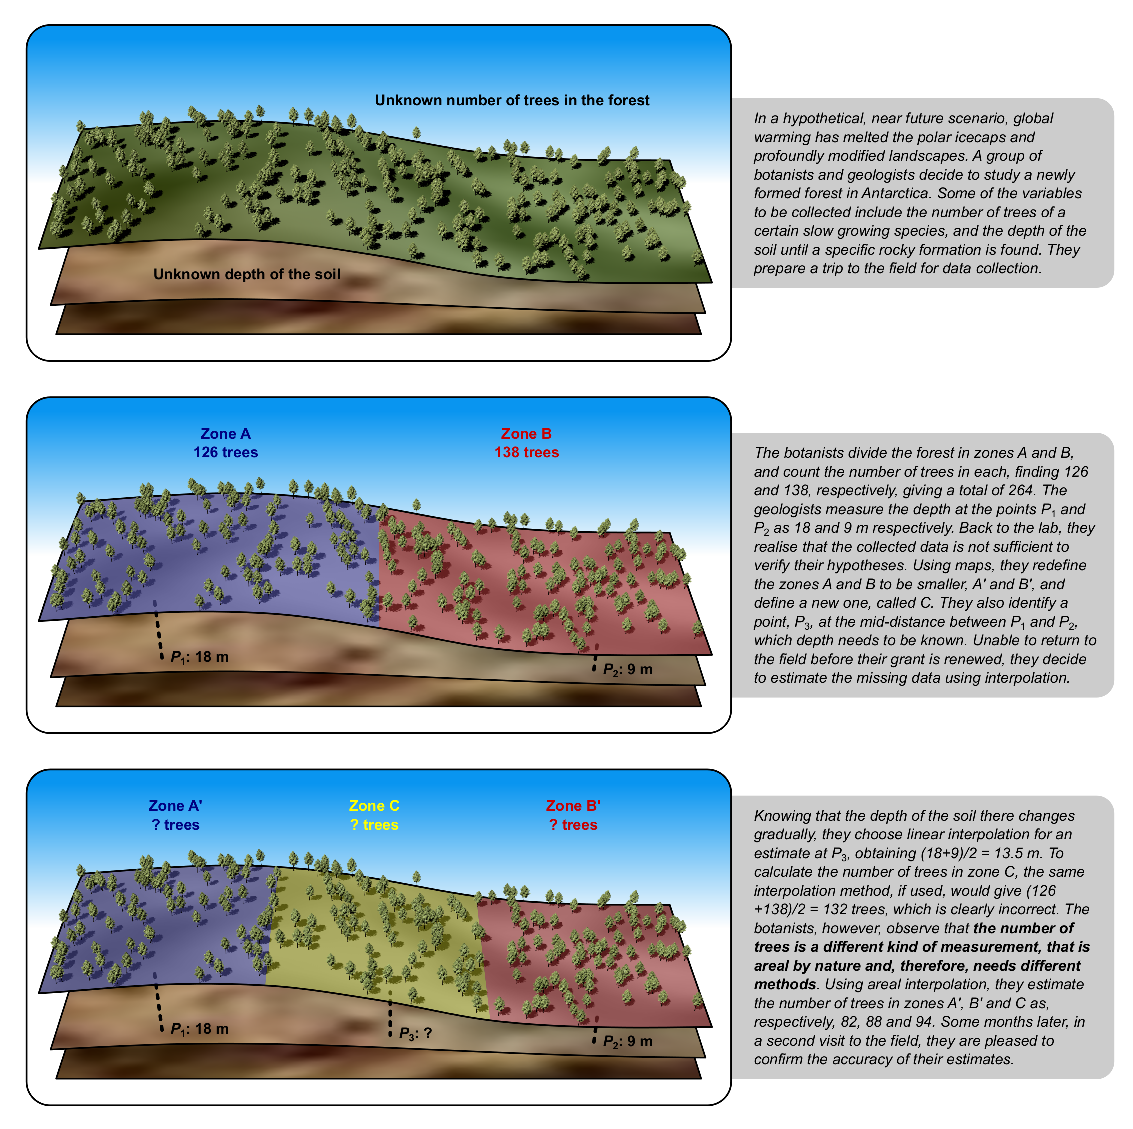
\includegraphics[width=14cm]{images/forest.eps}
\caption[Example demonstrating differences between area and point measurements.]{An example demonstrating differences in the nature of measurements. In this analogy, the depth of the soil is similar to brain cortical thickness, whereas the number of trees is similar to areal quantities distributed across the cortex. These areal quantities can be the surface area itself (in this case, the area of the terrain), but can also be any other measurement that is areal by nature (such as the number of trees).}
\label{fig:forest}
\end{figure}

\section{Method}

An overview of the method is presented in Figure~\ref{fig:overview}. Comparisons of cortical area between subjects require a surface model for the cortex to be constructed. A number of approaches are available \citep{Mangin1995, Dale1999, vanEssen2001, Kim2005} and, in principle, any could be used. Here we adopt the method of \citet{Dale1999} and \citet{Fischl1999_cortical}, as implemented in the FreeSurfer software package (\textsc{fs}).\footnote{Available at \href{http://surfer.nmr.mgh.harvard.edu}{http://surfer.nmr.mgh.harvard.edu}.} In this method, the $T_1$-weighted images are initially corrected for magnetic field inhomogeneities and skull-stripped \citep{Segonne2004}. The voxels belonging to the white matter (\textsc{wm}) are identified based on their locations, on their intensities, and on the intensities of the neighboring voxels. A mass of connected \textsc{wm} voxels is produced for each hemisphere, using a six-neighbors connectivity scheme, and a mesh of triangular faces is tightly built around this mass, using two triangles per exposed voxel face. The mesh is smoothed taking into account the local intensity in the original images \citep{Dale1993}, at a subvoxel resolution. Topological defects are corrected \citep{Fischl2001,Segonne2007} ensuring that the surface has the same topological properties of a sphere. A second iteration of smoothing is applied, resulting in a realistic representation of the interface between gray and white matter (the \emph{white surface}). The external cortical surface (the \emph{pial surface}), which corresponds to the pia mater, is produced by nudging outwards the white surface towards a point where the tissue contrast is maximal, maintaining constraints on its smoothness and on the possibility of self-intersection \citep{Fischl2000}. The white surface is inflated in an area-preserving transformation and subsequently homeomorphically transformed to a sphere \citep{Fischl1999_intersubject}. After the spherical transformation, there is a one-to-one mapping between faces and vertices of the surfaces in the native geometry (white and pial) and the sphere. These surfaces are comprised exclusively of triangular faces.

\begin{figure}[!p]  % Figure 2
\centering
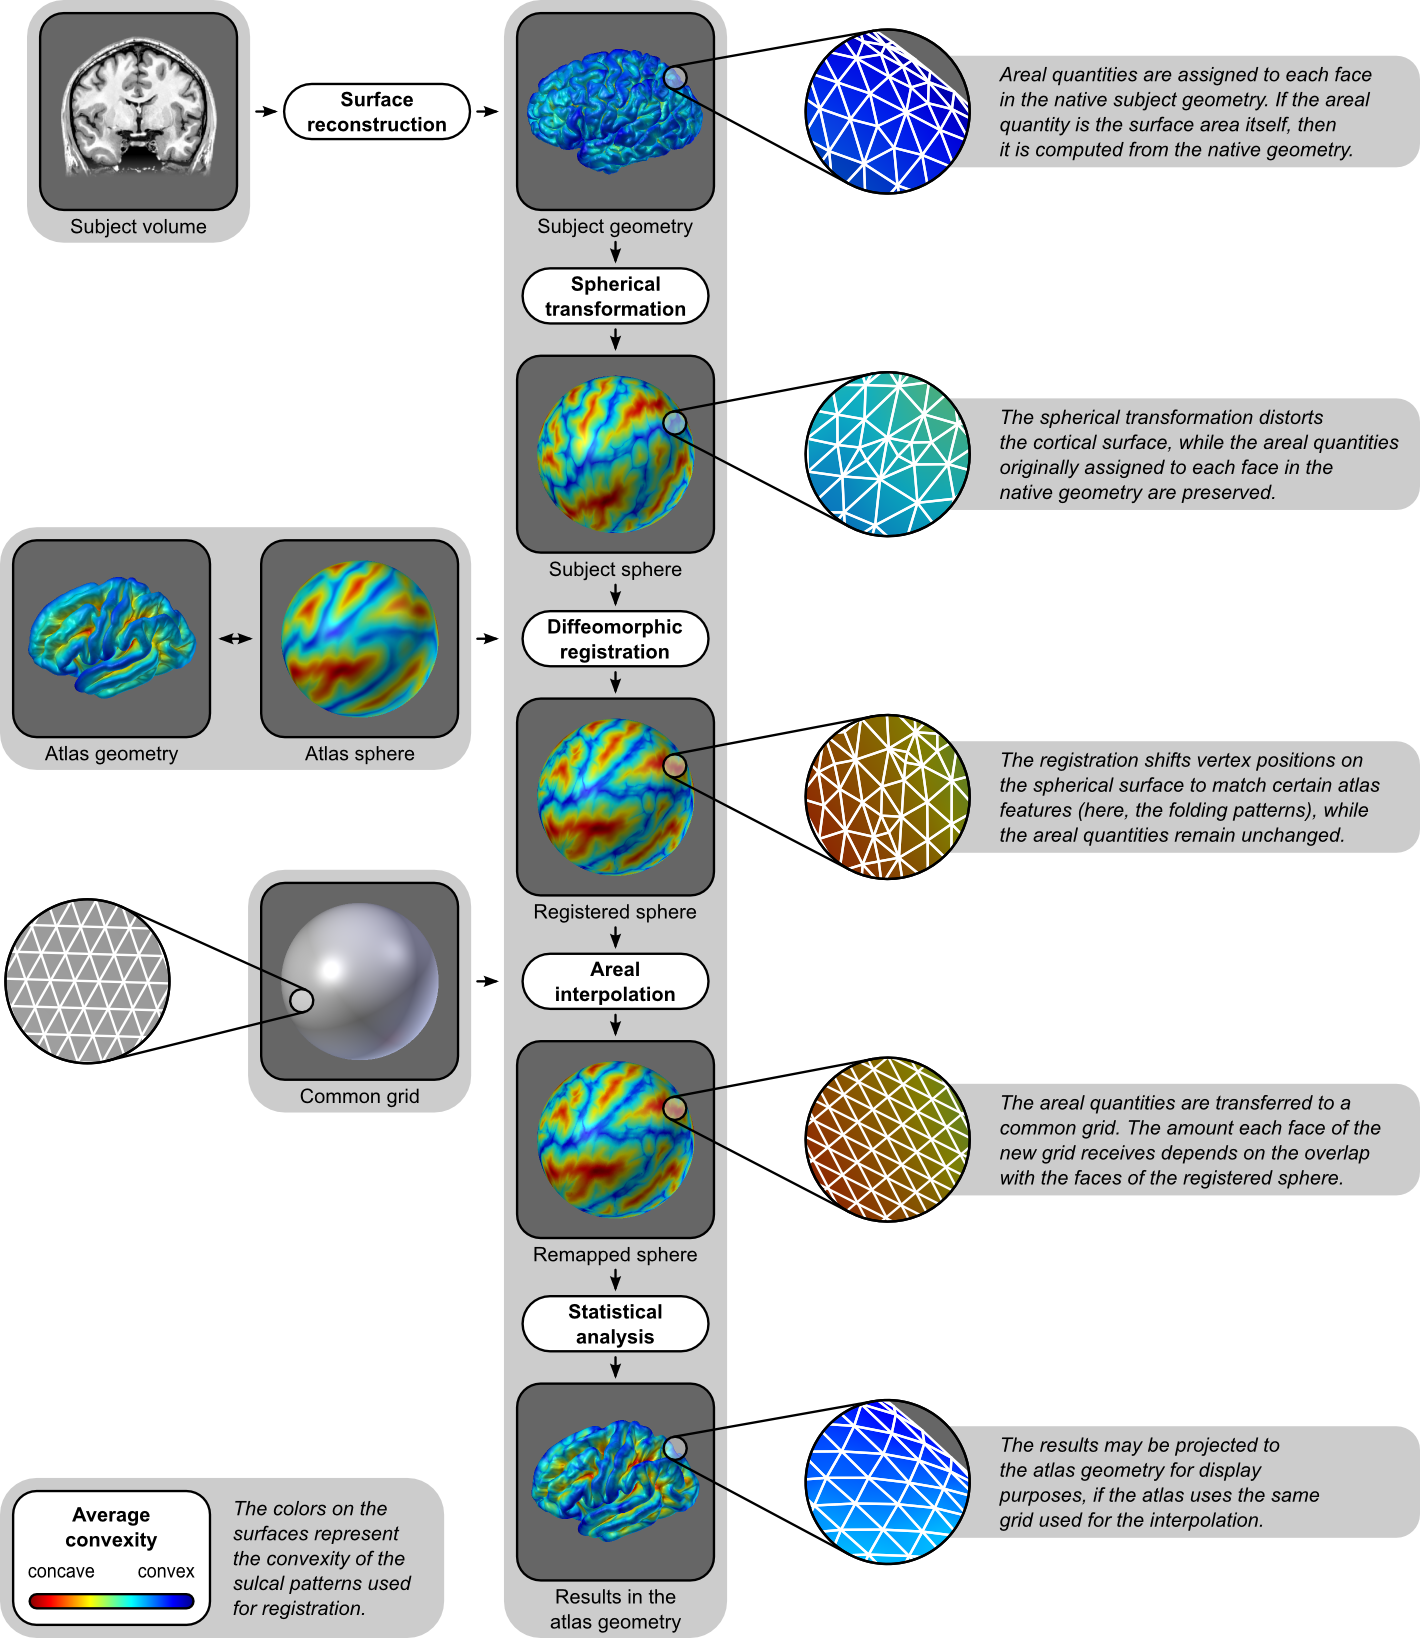
\includegraphics[width=14cm]{images/overview.png}
\caption[Overview of areal analyses.]{Diagram of the steps to analyse the cortical surface area. For clarity, the colors represent the convexity of the surface, as measured in the native geometry.}
\label{fig:overview}
\end{figure}

\subsection{Area per face and other areal quantities}

The surface area for analysis is computed at the interface between gray and white matter, i.e.\ at the \emph{white surface}. Another possible choice is to use the middle surface, i.e.\ a surface that runs at the mid-distance between white and pial. Although this surface is not guaranteed to match any specific cortical layer, it does not over or under-represent gyri or sulci \citep{vanEssen2005}, which might be an useful property. The white surface, on the other hand, matches directly a morphological feature and also tends to be less sensitive to cortical thinning or thickening than the middle or pial surfaces. Whenever methods to produce surfaces that represent biologically meaningful cortical layers are available, these should be preferred.

In contrast to conventional approaches in which the area of all faces that meet at a given vertex is summed and divided by three, producing a measure of the \emph{area per vertex}, for facewise analysis it is the \emph{area per face} that is measured and analysed. Since for each subject, each face in the native geometry has its corresponding face on the sphere, the value that represents area per face, as measured from the native geometry, can be mapped directly to the sphere, despite any areal distortion introduced by the spherical transformation.

Furthermore, since there is a direct mapping that is independent of the actual area in the native geometry, \emph{any other quantity that is biologically areal can also be mapped to the spherical surface}. Examples of such quantities, that may potentially be better characterized as areal processes, are the extent of the neural activation as observed with functional \textsc{mri}, the amount of cortical gray matter, the amount of amyloid deposited in Alzheimer's disease \citep{Klunk2004, Clark2011}, or simply the the number of cells counted from optic microscopy images reconstructed to a tri-dimensional space \citep{Schormann1998}. Since areal interpolation (described below) conserves locally, regionally and globally the quantities under study, it allows accurate comparisons and analyses across subjects for measurements that are areal by nature, or that require mass conservation on the surface of the mesh representation.

\subsection{Registration}

Registration to a common coordinate system is necessary to allow comparisons across subjects \citep{Drury1996}. The registration is performed by shifting vertex positions along the surface of the sphere until there is a good alignment between subject and template (target) spheres with respect to certain specific features, usually, but not necessarily, the cortical folding patterns. As the vertices move, the areal quantities assigned to the corresponding faces are also moved along the surface. The target for registration should be the less biased as possible in relation to the population under study \citep{Thompson2002}.

A registration method that produces a smooth, i.e.\ spatially differentiable, warp function enables the smooth transfer of areal quantities. A possible way to accomplish this is by using registration methods that are diffeomorphic. A diffeomorphism is an invertible transformation that has the elegant property that it and its inverse are both continuously differentiable \citep{Christensen1996, Miller1997}, minimising the risk of vagaries that would be introduced by the non-differentiability of the warp function.

Diffeomorphic methods are available for spherical meshes \citep{Glaunes2004, Yeo2010}, and here we adopt the Spherical Demons (\textsc{sd}) algorithm\footnote{Available at \href{http://sites.google.com/site/yeoyeo02/software/sphericaldemonsrelease}{http://sites.google.com/site/yeoyeo02/software/sphericaldemonsrelease}.} \citep{Yeo2010}. \textsc{Sd} extends the Diffeomorphic Demons algorithm \citep{Vercauteren2009} to spherical surfaces. The Diffeomorphic Demons algorithm is a diffeomorphic variant of the efficient, non-parametric Demons registration algorithm \citep{Thirion1998}. \textsc{Sd} exploits spherical vector spline interpolation theory and efficiently approximates the regularization of the Demons objective function via spherical iterative smooting.

Methods that are not diffeomorphic by construction, but in practice produce invertible and smooth warps could, in principle, be used for registration for areal analyses. In the Evaluation section we study the performance of different registration strategies as well as the impact of the choice of the template.

\subsection{Areal interpolation}

After the registration, the correspondence between each face on the registered sphere and each face from the native geometry is maintained, and the surface area or other areal quantity under study can be transferred to a common grid, where statistical comparisons between subjects can be performed. The common grid is a mesh which vertices lie on the surface of a sphere. A geodesic sphere, which can be constructed by iterative subdivision of the faces of a regular icosahedron, has many advantages for this purpose, namely, ease of computation, edges of roughly similar sizes and, if the resolution is fine enough, edge lengths that are much smaller than the diameter of the sphere (see Appendix~\ref{sec:geosphere} for details). These two spheres, i.e.\ the registered, irregular spherical mesh (source), and the common grid (target), typically have different resolutions. The interpolation method must, nevertheless, \emph{conserve the areal quantities}, globally, regionally and locally. In other words, the method has to be \emph{pycnophylactic}\footnote{From Greek \emph{pyknos} = mass, density, and \emph{phylaxis} = guard, protect, preserve, meaning that the method has to be mass conservative.} \citep{Tobler1979}. This is accomplished by assigning, to each face in the target sphere, the areal quantity of all overlapping faces from the source sphere, weighted by the fraction of overlap between them (Figure~\ref{fig:triangles}).

\begin{figure}[!t]  % Figure 3
\centering
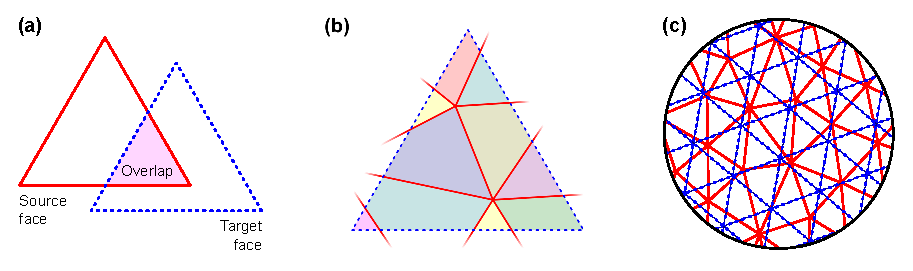
\includegraphics[width=14cm]{images/triangles.eps}
\caption[Overlapping areas used to weight areal quantities during interpolation.]{(a) Areal interpolation between a source and a target face uses the overlapping area as a weighting factor. (b) For a given target face, each overlapping source face contributes an amount of areal quantity. This amount is determined by the proportion between each overlapping area (represented in different colors) and the area of the respective source face. (c) The interpolation is performed at multiple faces of the target surface, so that the amount of areal quantity assigned to a given source face is conservatively redistributed across one or more target faces.}
\label{fig:triangles}
\end{figure}

More specifically, let $Q^{S}_{i}$ represent the areal quantity on the $i$-th face of the registered, source sphere $S$, $i=1,2,\ldots,I$. This areal quantity can be directly mapped back to the native geometry, and can be the area per face as measured in the native geometry, or any other quantity of interest that is areal by nature. Let the actual area of the same face on the source sphere be indicated by $A^{S}_{i}$. The quantities $Q^{S}_{i}$ have to be transfered to a target sphere $T$, the common grid, which face areas are given by $A^{T}_{j}$ for the $j$-th face, $j=1,2,\ldots,J$, $J \neq I$. Each target face $j$ overlaps with $K$ faces of the source sphere, being these overlapping faces indicated by indices $k=1,2,\ldots,K$, and the area of each overlap indicated by $A^{O}_{k}$. The interpolated areal quantity to be assigned to the $j$-th target face is then given by:

\begin{equation}
Q^{T}_{j} = \sum_{k=1}^{K} \frac{A^{O}_{k}}{A^{S}_{k}} Q^{S}_{k}
\end{equation}

Similar interpolation schemes have been devised to solve problems in geographic information systems (\textsc{gis}) \citep{Markoff1973, Goodchild1980, Flowerdew1991, Gregory2010}. Surface models of the brain impose at least one additional challenge, which we address in the implementation (see Appendix~\ref{sec:implementation}). Differently than in other fields, where interpolation is performed over geographic territories that are small compared to Earth and, therefore, can be projected to a plane with acceptable areal distortion, here we have to interpolate across the whole sphere. Although other conservative interpolation methods exist for this purpose \citep{Jones1999, Lauritzen2008, Ullrich2009}, these methods either use regular latitude-longitude grids, cubed-spheres, or require a special treatment of points located above a certain latitude threshold to avoid singularities at the poles. These disadvantages may render these methods suboptimal for direct use in brain imaging.

\subsection{Geodesic spheres and areal inequalities}
\label{sec:geosphere}

The only required feature for the common grid used for the areal interpolation is that all its vertices must lie on the surface of a sphere. The algorithm we present in Appendix~\ref{sec:implementation} requires further that all faces of the sphere are triangular and that all edges of all faces are much smaller than the radius, so that areal distortion is minimised when projecting to a plane.

A common grid that meet these demands is a sufficiently fine geodesic sphere. There are different ways to construct such a sphere \citep{Kenner1976}. One method is to subdivide each face of a regular polyhedron with triangular faces, such as the icosahedron, into four new triangles. The new vertices are projected to the surface of the (virtual) circumscribed sphere along its radius and the process is repeated recursively a number of times \citep{Lauchner1969}. For the $n$-th iteration, the number of faces is given by $F=4^nF_0$, the number of vertices by $V=4^n(V_0-2)+2$, and the number of edges by $E=4^nE_0$, where $F_0$, $V_0$ and $E_0$ are, respectively, the number of faces, vertices and edges of the polyhedron with triangular faces used for the initial subdivision. For the icosahedron, $F_0=20$, $V_0=12$ and $E_0=30$ (Figure~\ref{fig:geosphere}\emph{a}). For the analyses in this manuscript, we used $n=7$, producing geodesic spheres with 327680 faces and 163842 vertices.

These faces, however, do not have identical edge lengths and areas \citep{Kenner1976}, even though the initial icosahedron was perfectly regular. This is important for areal interpolation, as larger faces on the target grid do overlap with more faces from the source surfaces, absorbing larger amounts of areal quantities, possibly causing confusion if one attempts to color-encode the interpolated image according to the actual areal quantities, in which case, geometric patterns such as in Figure~\ref{fig:geosphere}\emph{b} will become evident. Moreover, smoothing can cause quantities that are arbitrarily large or small due to face sizes to be blurred into the neighbors. Both potential problems can be addressed by multiplying the areal quantity at each face $j$, after interpolation, by a constant given by $4 \pi r^2/(A^{T}_{j}F)$, where $A^{T}_{j}$ is the area of the same face of the geodesic sphere, $F$ is the number of faces, and $r$ is the radius of the sphere.

\begin{figure}[!t]  % Figure 11
\centering
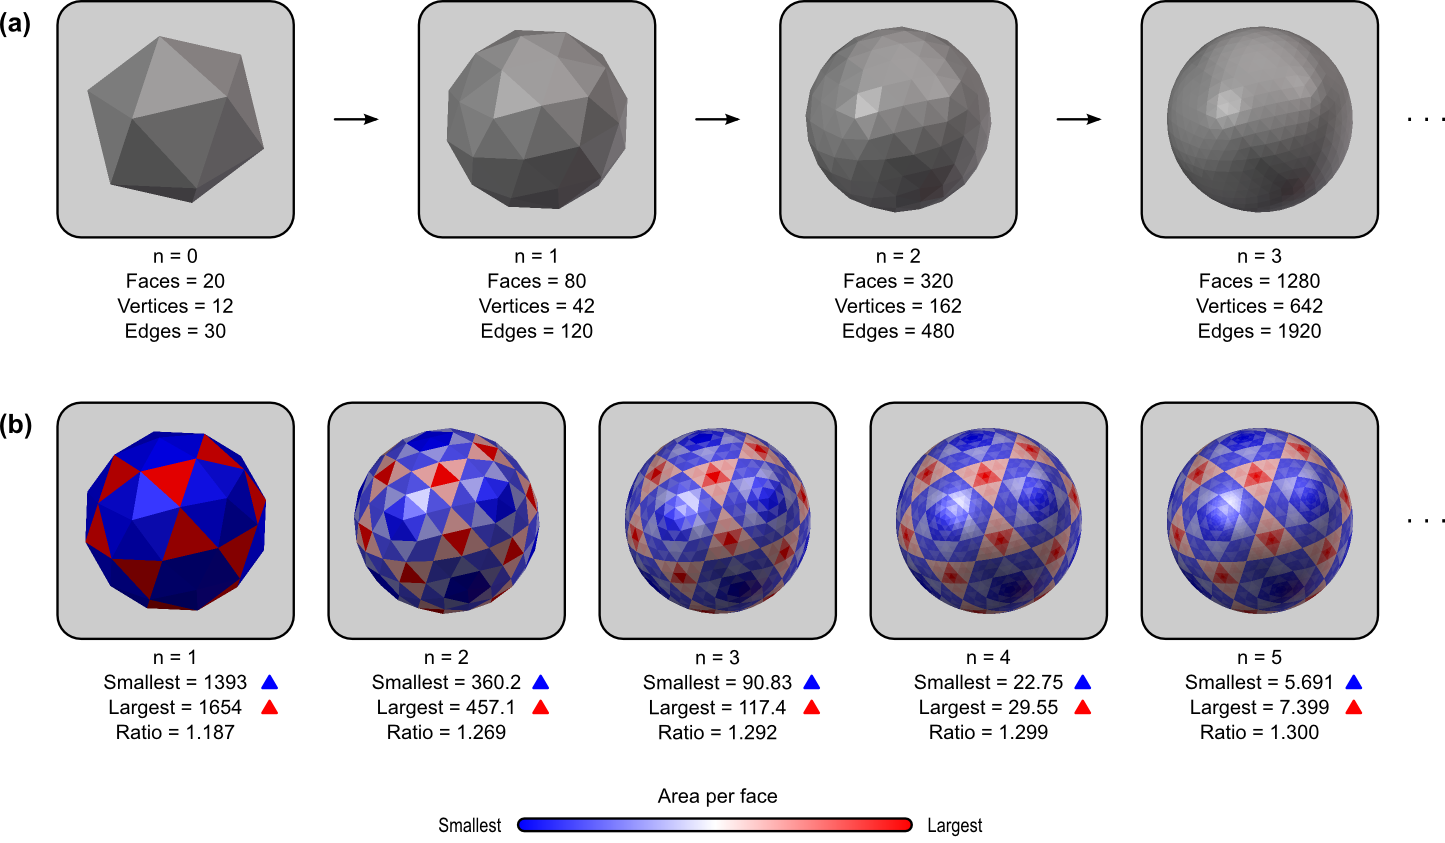
\includegraphics[width=14cm]{images/geosphere.png}
\caption[Geodesic spheres.]{(a) The common grid can be a geodesic sphere produced from recursive subdivision of a regular icosahedron. At each iteration, the number of faces is quadruplied. (b) After the first iteration, however, the faces no longer have regular sizes, with the largest face being approximately 1.3 times larger than the smallest as $n$ increases.}
\label{fig:geosphere}
\end{figure}

\subsection{Smoothing}
\label{sec:smoothing}

Smoothing can be applied to alleviate residual discontinuities in the interpolated data due to unfavorable geometric configurations between faces of source and target spheres. For the purpose of smoothing, facewise data can be represented either by their barycenters, or converted to vertexwise (see Appendix~\ref{sec:presentation} for a discussion on how to convert), and should take into account differences on face sizes, as larger faces will tend to absorb more areal quantities (see Appendix~\ref{sec:geosphere}). Smoothing can be applied using the moving weights method \citep{Lombardi2002}, defined as

\begin{equation}
\tilde{Q}^{T}_n = \frac{\sum_j Q^{T}_j G(g(\mathbf{x}_n,\mathbf{x}_j))}{\sum_j G(g(\mathbf{x}_n,\mathbf{x}_j))}
\end{equation}

\noindent where $\tilde{Q}^{T}_n$ is the smoothed areal quantity at the $n$-th face, $Q^{T}_j$ is the areal quantity assigned to each of the $J$ faces of the same surface before smoothing, $g(\mathbf{x}_n,\mathbf{x}_j)$ is the scalar-valued distance along the surface between the barycenter $\mathbf{x}_n$ of the current face and the barycenter $\mathbf{x}_j$ of another face, and $G(g)$ is the Gaussian kernel.\footnote{As with other neuroimaging applications, smoothing after registration implies that the effective filter width is not spatially constant in native space, neither is the same across subjects. Smoothing on the sphere also contributes to different filter widths across space due to the deformation during spherical transformation.}

\subsection{Conversion from facewise to vertexwise}
\label{sec:conversion}

Whenever it is necessary to perform analyses that include measurements taken at each vertex (such as some areal quantity versus cortical thickness) or when only software that can display vertexwise data is available (Appendix~\ref{sec:presentation}, it may be necessary to convert the areal quantities from facewise to vertexwise. The conversion can be done by redistributing the quantities at each face to their three constituent vertices. The areal values assigned to the faces that meet at a given vertex are summed, and divided by three, and reassigned to this vertex. Importantly, this procedure has to be done \emph{after} the areal interpolation, since interpolation methods for vertexwise data are not appropriate for areal quantities, and \emph{before} the statistical analysis, since the average of the results of the statistics of a test is not necessarily the same as the statistic for the average of the original data. It should also be observed that conversion from facewise to vertexwise data implies a loss of resolution to approximately half of the original and, therefore, should be performed only if resolution is not a concern and there is no other way to analyse, visualize, or present facewise data or results. The conversion does not change the underlying distribution, provided that the resolution of the initial mesh is sufficiently fine.

\subsection{Statistical analysis}

After resampling to a common grid, the facewise data is ready for statistical analysis. The most straightforward method is to use the general linear model (\textsc{glm}). The \textsc{glm} is based on a number of assumptions, including that the observed values have a linear, additive structure, that the residuals of the model fit have the same variance and are normally distributed. When these assumptions are not met, a non-linear transformation can be applied, as long as the true, biological or physical meaning that underlies the observed data is preserved. In the Evaluation section, we show empirically that facewise cortical surface area is largely not normal. Instead, the distribution is skewed and can be better characterized as \emph{lognormal}. A generic framework that can accommodate arbitrary areal quantities with skewed distributions is using a power transformation, such as the Box--Cox transformation \citep{Box1964}, which addresses possible violations of these specific assumptions, allied with permutation methods for inference \citep{Holmes1996, Nichols2003} when the observations can be treated as independent, such as in most between-subject analysis.

The application of a statistical test at each face allows the creation of a statistical map and also introduces the multiple testing problem, which can also be addressed using permutation methods. These methods are known to allow exact significance values to be computed, even when distributional assumptions cannot be guaranteed, and also to facilitate strong control over family-wise error rate (\textsc{fwer}) if the distribution of the statistic under the null hypothesis is similar across tests. If not similar, the result is still valid, yet conservative. An alternative is to use a relatively assumption-free approach to address multiple testing, controlling instead the false discovery rate (\textsc{fdr}) \citep{Benjamini1995, Genovese2002}, which offers also weak control over \textsc{fwer}. Other approaches for inference, such as the Random Field Theory (\textsc{rft}) for meshes \citep{Worsley1999, Hagler2006} and the Threshold-Free Cluster Enhancement (\textsc{tfce}) \citep{Smith2009} have potential to be used, although due to reliance on stringent assumptions or dependence upon specification of certain parameters, these methods need yet a careful evaluation for facewise areal quantities. Strategies to present results are discussed in Appendix~\ref{sec:presentation}.

\subsection{Presentation of results}
\label{sec:presentation}

To display results, facewise data can be projected from the common grid to the template geometry, which helps to visually identify anatomical landmarks and name structures. Projecting data from one surface to another is trivial as there is a one-to-one mapping between faces of the grid and the template geometry. The statistics and associated p-values can be encoded in colors, and a color scale can be shown along with the surface model.

However, the presentation of facewise data has conceptual differences in comparison with the presentation vertexwise data. For vertexwise data, each vertex cannot be directly colored, for being dimensionless. Instead, to display data per vertex, typically each face has its color interpolated according to the colors of its three defining vertices, forming a linear gradient that covers the whole face. For facewise data there is no need to perform such interpolation of colors, since the faces can be shown directly on the \textsc{3d} space, each one in the uniform color that represents the underlying data. The difference is shown in Figure~\ref{fig:display}.

\begin{figure}[!tp]  % Figure 12
\centering
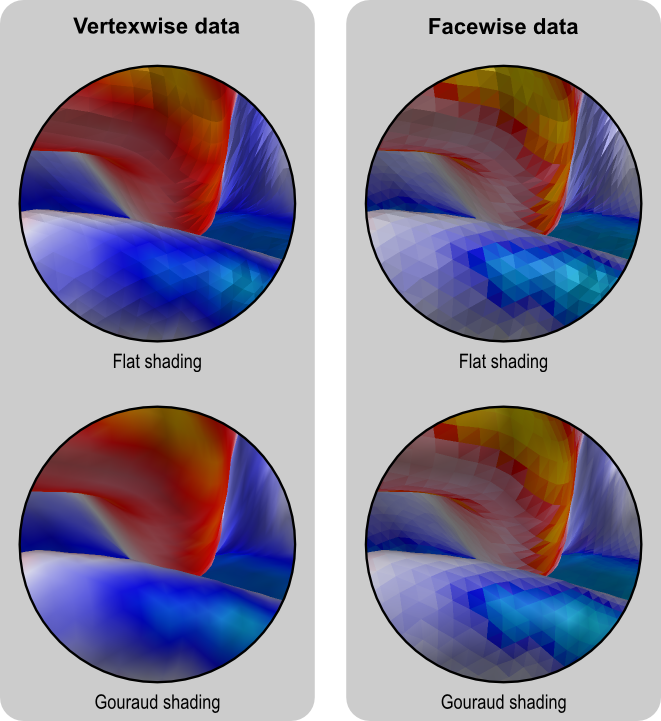
\includegraphics[width=9cm]{images/display.png}
\caption[Differences between presentation of facewise and vertexwise area.]{Differences between presentation of facewise and vertexwise data can be observed in this zoomed portion of the mesh representation of the cortex. Vertices are dimensionless and, to display vertexwise data, the faces have to be colored using linear interpolation. This is not necessary for facewise data, which can be shown directly in the uniform colors that represent the underlying data. In either case, the presentation can be improved by using a shading model, such as Gouraud in this example. Although the vertexwise presentation may be visually more appealing, it contains only half the resolution of the facewise image.}
\label{fig:display}
\end{figure}

Interpolation of colors for vertexwise data should not be confused with the related, yet different concept of lightning and shading using interpolation. Both vertexwise and facewise data can be shaded to produce more realistic images. In Figure~\ref{fig:display} we give an example of simple flat shading and shading based on linear interpolation of the lightning at each vertex \citep{Gouraud1971}.

Currently available software allow the presentation of color-encoded vertexwise data on the surface of meshes. However, only very few software applications can handle a large number of colors per \textsc{3d} object, being one color per face. One example is Blender (Blender Foundation, Amsterdam, The Netherlands), which we used to produce the figures presented in this article. Another option, for instance, is to use low-level mesh commands in \textsc{matlab}, such as \texttt{patch}.

\subsection{Implementation}
\label{sec:implementation}

The areal interpolation for spheres is implemented in two parts. In the first, we compute inside of which source faces the target vertices are located, creating a lookup table to be used in the second part. This is the point-in-polygon problem found in vector graphics applications \citep{Vince2005}. Here we calculate the area of each source face, $A^{S}_{i}$, and the subsequent steps proceed iteratively for each face in the source. The barycentric coordinates of each candidate vertex in relation to the current face $i$ is computed; if their sum equals to unity, the point is labelled as inside. However, to test if all vertices are inside every face would needlessly waste computational time. Moreover, since all points are on the surface of a sphere, the vertices in the target are never expected to be coplanar to the source triangular faces, so the test would always fail. The first problem is treated by testing only the vertices located within a bounding box defined, still in the \textsc{3d} space, from the source face extreme coordinates. The second could na\"{i}vely be treated by converting the \textsc{3d} Cartesian coordinates to \textsc{2d} spherical coordinates, which allow a fast flattening of the sphere to the popular plate carr\'{e}e cylindrical projection. However, latitude is ill-defined at the poles in cylindrical projections. Moreover, cylindrical projections introduce a specific type of deformation that is undesired here: straight lines on the surface (geodesic lines) are distorted. The solution we adopt is to rotate the Cartesian coordinate system so that the barycenter of the current source face lies at the point $(r,0,0)$, where $r$ is the radius of the source and target spheres. The barycenter is used for ease of calculation and for being always inside the triangle. After rotation, the current face and the nearby candidate target vertices are projected to a plane using the azimuthal gnomonic projection \citep{Snyder1987}, centered at the barycenter of the face. The point-in-polygon test can then be applied successfully. The key advantage of the gnomonic projection is that all geodesics project as straight lines, rather than loxodromic or other complex paths as with other projections, which would cause many target vertices to be incorrectly labelled. This projection can be obtained trivially after the rotation of the \textsc{3d} Cartesian coordinate system as $\phi=y/x$ and $\theta=z/x$, where $(x,y,z)$ are the \textsc{3d} coordinates of the point being projected. A potential disadvantage of the gnomonic projection is the remarkable areal distortion for regions distant from the center of the projection. Since in typical neuroimaging applications the source and target spheres are composed of a tessellation of approximately $3\times10^6$ faces, $A^{S}_{i} \ll 4 \pi r^2$, and the distortion becomes negligible.

In the second part, the areal interpolation is performed, with the overlapping areas being calculated and used to weigh the areal quantity under study. The identification of intersections between two sets of polygons is also a well studied problem in vector graphics \citep{Guibas1987, Chazelle1994}, which solution depends on optimally finding crossings between multiple line segments \citep{Bentley1979, Chazelle1992, Balaban1995}. Most of the efficient available algorithms assume that the polygons are all coplanar; those that work in the surface of a sphere use coordinates expressed in latitude and longitude and require special treatment of the polar regions. The solution we adopt obviates these problems by first computing the area of each target face, $A^{T}_{j}$; the subsequent steps are performed iteratively for each face in the target sphere, using the azimuthal gnomonic projection, similarly as in the first part, but now centered at the barycenter of the current target face at every iteration. The areal quantities assigned to the faces in the target sphere are initialized as zero before the loop begins. If all three vertices of the current target face $j$ lie inside the same source face $k$, as known from the lookup table produced in the first part, then to the current face the areal quantity given by $Q^{T}_{j} = Q^{S}_{k} A^{T}_{j} / A^{S}_{k}$ is assigned. Otherwise, the source faces that surround the target are examined to find overlaps. This is done by considering the edges of the current target face as vectors organised in counter-clockwise orientation, and testing if the vertices of the candidate faces lie on the left, right or if they coincide with the edge. If all the three vertices of any candidate face are on the right of any edge, there is no overlap and the candidate face is removed from further consideration. If all the three vertices are on the left of all three edges, then the candidate source face is entirely inside the target, which has then its areal quantity incremented as $Q^{T}_{j} \leftarrow Q^{T}_{j} + Q^{S}_{k}$. The remaining faces are those that contain some vertices on the left and some on the right of the edges of the current, target face. The intersections between these source and target edges are computed and false intersections between edge extensions are ignored. A list containing the vertices for each candidate source face that are inside the target face (known for being on the left of the three target edges), the target vertices that are inside each of the source faces (known from the lookup table) and the coordinates of the intersections between face edges, is used to compute the convex hull, using the Quickhull algorithm \citep{Barber1996}. The convex hull delimits the overlapping region between the current target face $j$ and the candidate source face $k$, which area, $A^{O}_{k}$, is used to increment the areal quantity assigned to the target face as $Q^{T}_{j} \leftarrow Q^{T}_{j} + Q^{S}_{k} A^{O}_{k}/A^{S}_{k}$.

The algorithm runs in $\mathcal{O}(n)$ for $n$ faces, as opposed to $\mathcal{O}(n^2)$ that would be obtained by na\"ive search. Nevertheless, the current implementation in Octave/\textsc{matlab}, a dynamically typed, interpreted language, requires about 24 hours to run in a computer with 2.66~GHz Intel Xeon processors.


\section{Evaluation}

We illustrate the method using data from the Genetics of Brain Structure and Function Study, \textsc{gobs}, a collaborative effort involving the Texas Biomedical Institute, the University of Texas Health Science Center at San Antonio (\textsc{uthscsa}) and the Yale University School of Medicine. The participants are members of 42 families, and total sample size, at the time of the selection for this study, is 868 subjects. We randomly chose 84 subjects (9.2\%), with the sparseness of the selection minimizing the possibility of drawing related individuals. The mean age of these subjects was 45.1 years, standard deviation 13.9, range 18.2--77.5, with 33 males and 51 females. All participants provided written informed consent on forms approved by each Institutional Review Board. The images were acquired using a Siemens \textsc{magnetom} Trio 3~T system (Siemens \textsc{ag}, Erlangen, Germany) for 46 participants, or a Siemens \textsc{magnetom} Trio/\textsc{tim} 3~T system for 38 participants. We used a $T_1$-weighted, \textsc{mprage} sequence with an adiabatic inversion contrast pulse with the following scan parameters: $\textsc{te}/\textsc{ti}/\textsc{tr}$~= 3.04/785/2100~ms, flip angle~= 13$^{\circ}$, voxel size (isotropic)~= 0.8~mm. Each subject was scanned 7 (seven) times, consecutively, using the same protocol, and a single image was obtained by linearly coregistering these images and computing the average, allowing improvement over the signal-to-noise ratio, reduction of motion artifacts \citep{Kochunov2006}, and ensuring the generation of smooth, accurate meshes with no manual intervention. The image analysis followed the steps described in the Methods section, with some variation to test different registration strategies.

\subsection{Registration}

To isolate and evaluate the effect of registration, we computed the area per face after the spherical transformation\footnote{Note that here the area was computed in the sphere with the aim of evaluating the registration method. For analyses of areal quantities, these quantities should be defined in the native geometry, as previously described.} and registered each subject brain hemisphere to a common target using two different registration methods, the Spherical Demons \citep{Yeo2010} and the FreeSurfer registration algorithm \citep{Fischl1999_intersubject}\footnote{The software versions used were \textsc{fs} 5.0.0 and \textsc{sd} 1.5.1.}, each with and without a study-specific template as the target, resulting in four different variants. The study-specific targets for each of these methods were produced using the respective algorithms for registration, using all the 84 subjects from the sample. The non-specific target was derived from an independent set of brain images of 40 subjects, the details of which have been described elsewhere \citep{Desikan2006}. Areal interpolation was used to resample the areal quantities to a common grid, a geodesic sphere produced by seven recursive subdivisions of a regular icosahedron.

The average area per face across subjects was computed after registration and interpolation to identify eventual systematic patterns of distortion caused by warping. This can be understood by observing that, as the vertices are shifted along the surface of the sphere, the faces that they define, and which carry areal quantities, are also shifted and distorted. The registration, therefore, causes displacement of areal quantities across the surface, which may accumulate on certain regions while other become depleted. Ideally, there should be no net accumulation when many subjects are considered and the target is unbiased with respect to the population under study. If pockets of accumulated or depleted areal quantities are present, this means that some regions are showing a tendency to systematically ``receive'' more areal quantities than others, which ``donate'' quantities. The average amount of area after the registration estimates this accumulation and, therefore, can be used as a measure of a specific kind of bias in the registration process, in which some regions consistently attract more vertices, resulting in these regions receiving more quantities. The result for this analysis is shown in Figure~\ref{fig:registration}. Using default settings, \textsc{sd} caused less areal displacement across the surface, with less regional variation when compared to \textsc{fs}. The pattern was also more randomly distributed for \textsc{sd}, without spatial trends matching anatomical features, whereas \textsc{fs} showed a structure more influenced by brain morphology. Using a study specific template further helped to reduce areal shifts and biases. The subsequent analyses we present are based on the \textsc{sd} registration with a study-specific template.

\begin{figure}[!p]  % Figure 4
\centering
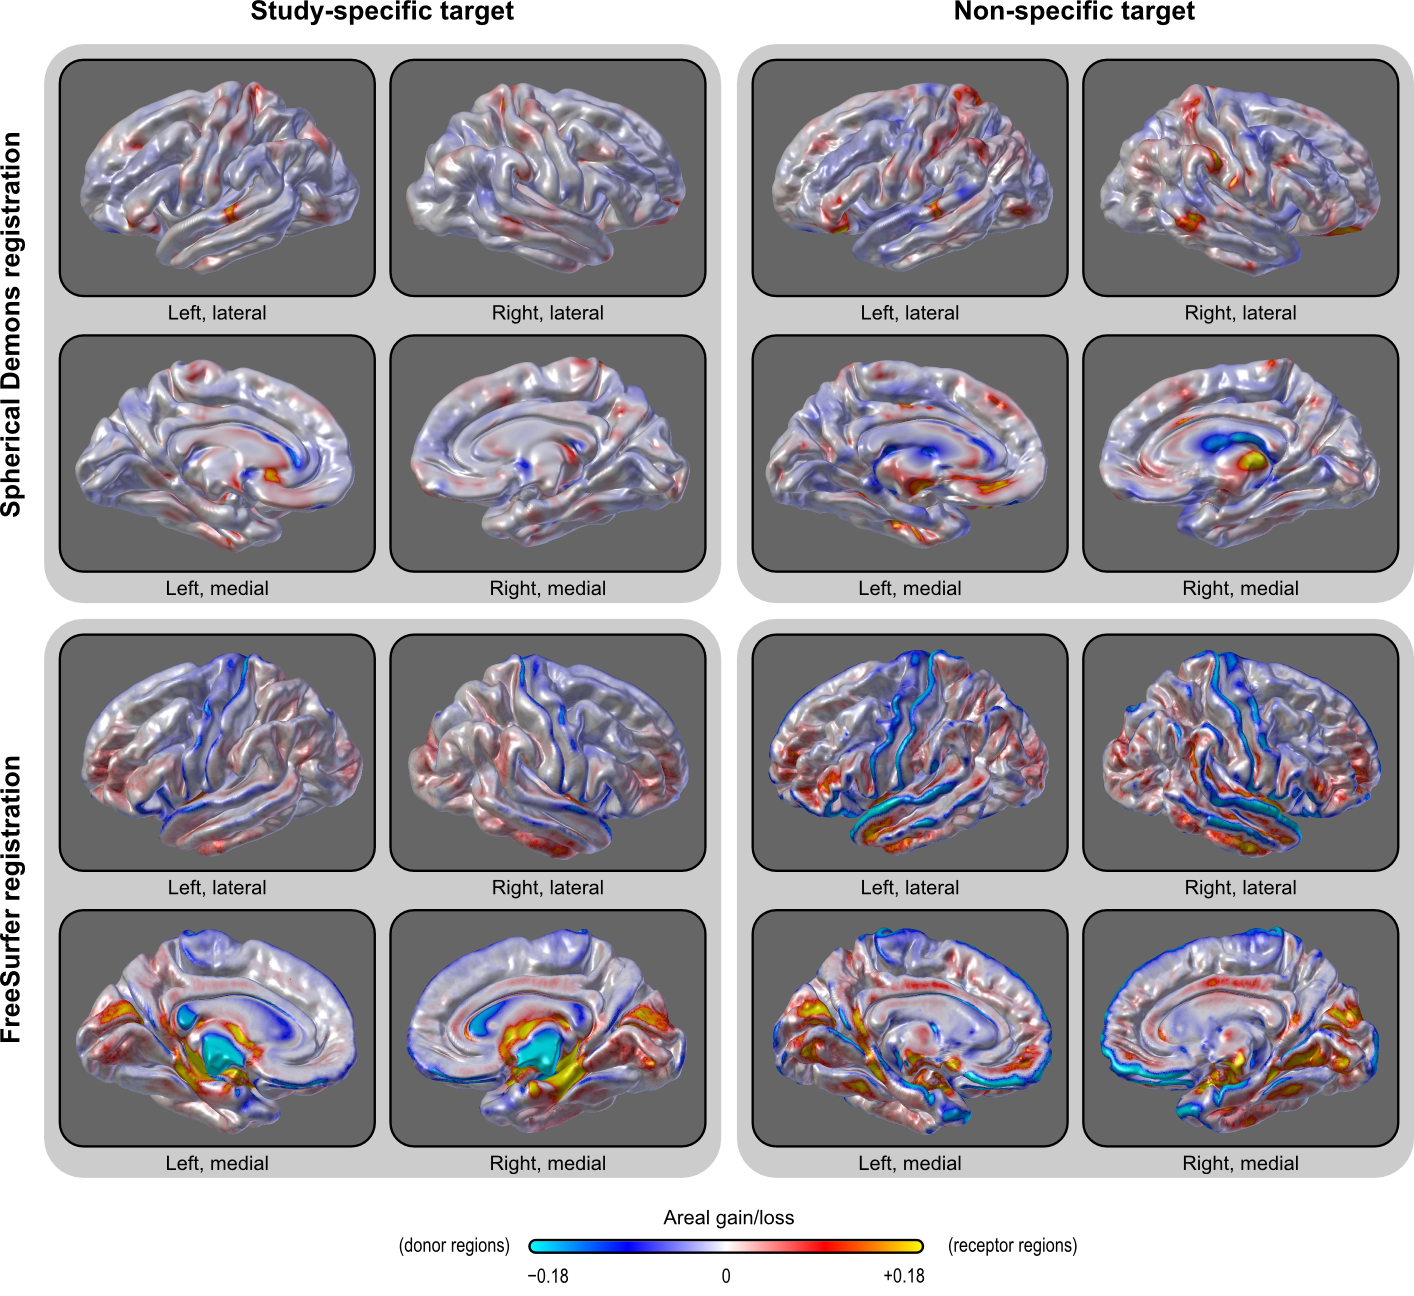
\includegraphics[width=14cm]{images/registration.png}
\caption[Effect of registration method on areal analyses.]{A study-specific template (target for the registration) caused less systematic accumulation of areal quantities across the brain when compared with a non-specific template. Using default parameters, areal accumulation wa less pronounced and unrelated to sulcal patterns using Spherical Demons in comparison with FreeSurfer registration. Gains and losses refer to the area per face that would be expected for areal quantities being redistributed with no bias, i.e. the zero corresponds to the average total surface area of all subjects, divided by the number of faces.}
\label{fig:registration}
\end{figure}

\subsection{Distributional characterization}

To evaluate the normality for the cortical area at the white surface of the native geometry, we used the Shapiro--Wilk normality test \citep{Shapiro1965}, implemented with the approximations for samples larger than 50 as described by \citet{Royston1993}. The test was applied after each hemisphere of the brain was registered to a study-specific template using the Spherical Demons and interpolated to the geodesic sphere using areal interpolation.

For the vast majority of the faces, the area of the white surface is \emph{not} normally distributed (Figures~\ref{fig:shapiro}--\ref{fig:kurtosis-hist}). Instead, the lognormal distribution seems to be more appropriate to describe the data in most parts of the brain, with the test declaring a much larger number of faces as normally distributed after a simple logarithmic transformation. A log-transformation is a particular case of the Box--Cox transformation \citep{Box1964}. For a set of values $y=\left\{ y_1, y_2, \ldots , y_n \right\}$, this transformation uses maximum-likelihood methods to seek a parameter $\lambda$ that produces a transformed set $\tilde{y}=\left\{ \tilde{y}_1, \tilde{y}_2, \ldots , \tilde{y}_n \right\}$ that approximately conforms to a normal distribution. The transformation is a piecewise function given by:

\begin{equation}
\tilde{y} = \left\{ \begin{array}{ll}
\dfrac{y^{\lambda}-1}{\lambda} & (\lambda \neq 0) \\
\ln y & (\lambda = 0)
\end{array} \right.
\end{equation}

Not surprisingly, the Box--Cox transformation rendered the data more normally distributed than a simple log-transformation. However, an interesting aspect of this transformation is that the parameter $\lambda$ is allowed to vary continuously, and it approaches unity when the data is normally distributed, and zero if lognormally distributed, serving, therefore, as a summary metric of how normally or lognormally distributed the data is. Throughout most of the brain, $\lambda$ is close to zero, although with a relatively wide variation (mode = $-0.057$, mean = $-0.099$, sd = $0.493$ for the analysed dataset), indicating that, at the resolution used, the white surface cortical area can be better characterized across the surface as a gradient of skewed distributions, with the lognormal being the most common case. The same was observed for facewise data smoothed in the sphere after interpolation with \textsc{fwhm} = 10~mm (mode = $-0.142$, mean = $-0.080$, sd = $0.578$).\footnote{For scale comparison, the sphere has radius fixed and set as 100~mm, such that the Gaussian filter has an \textsc{hwhm} (half width) = 1.59\% of the geodesic distance between the barycenter of any face and its antipode.} Maps for the parameter $\lambda$ are shown in Figure~\ref{fig:boxcox}.

% \begin{figure}[!p]  % Figure 5
% \centering
% 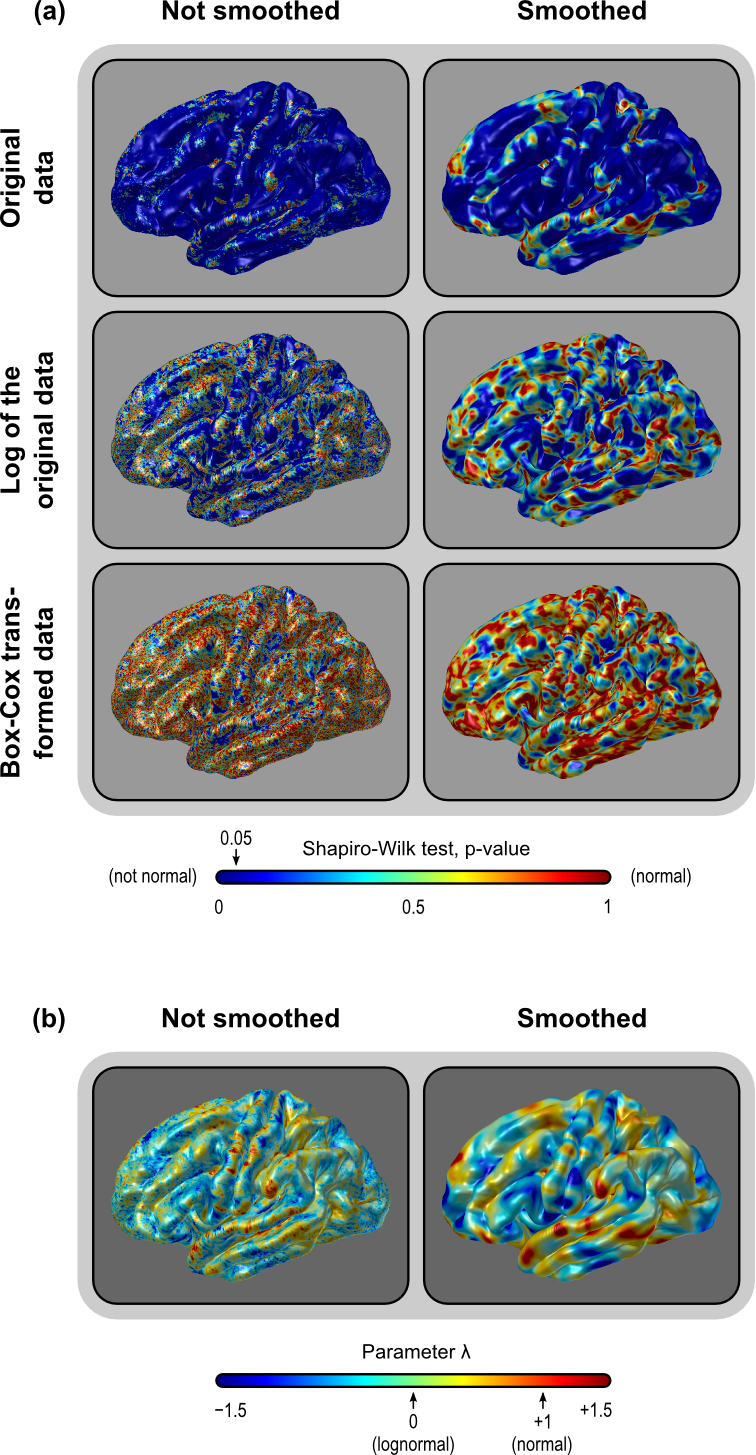
\includegraphics[width=9cm]{images/shapiro-simpl.png}
% \caption[The distribution of surface area is lognormal.]{(a) The area of the cortical surface is not normally distributed (upper panels). Instead, it is lognormally distributed throughout most of the brain (middle panels). A Box--Cox transformation can further improve normality (lower panels). The same pattern is present without (left) or with (right) smoothing (\textsc{fwhm} = 10~mm). (b) Spatial distribution of the parameter $\lambda$ across the brain. When $\lambda$ approaches zero, the distribution is more lognormal. See the Supplemental Material for the other views of the brain and histograms for $\lambda$.}
% \label{fig:shapiro-simpl}
% \end{figure}

\begin{figure}[!p]  % Figure Suppl 1
\centering
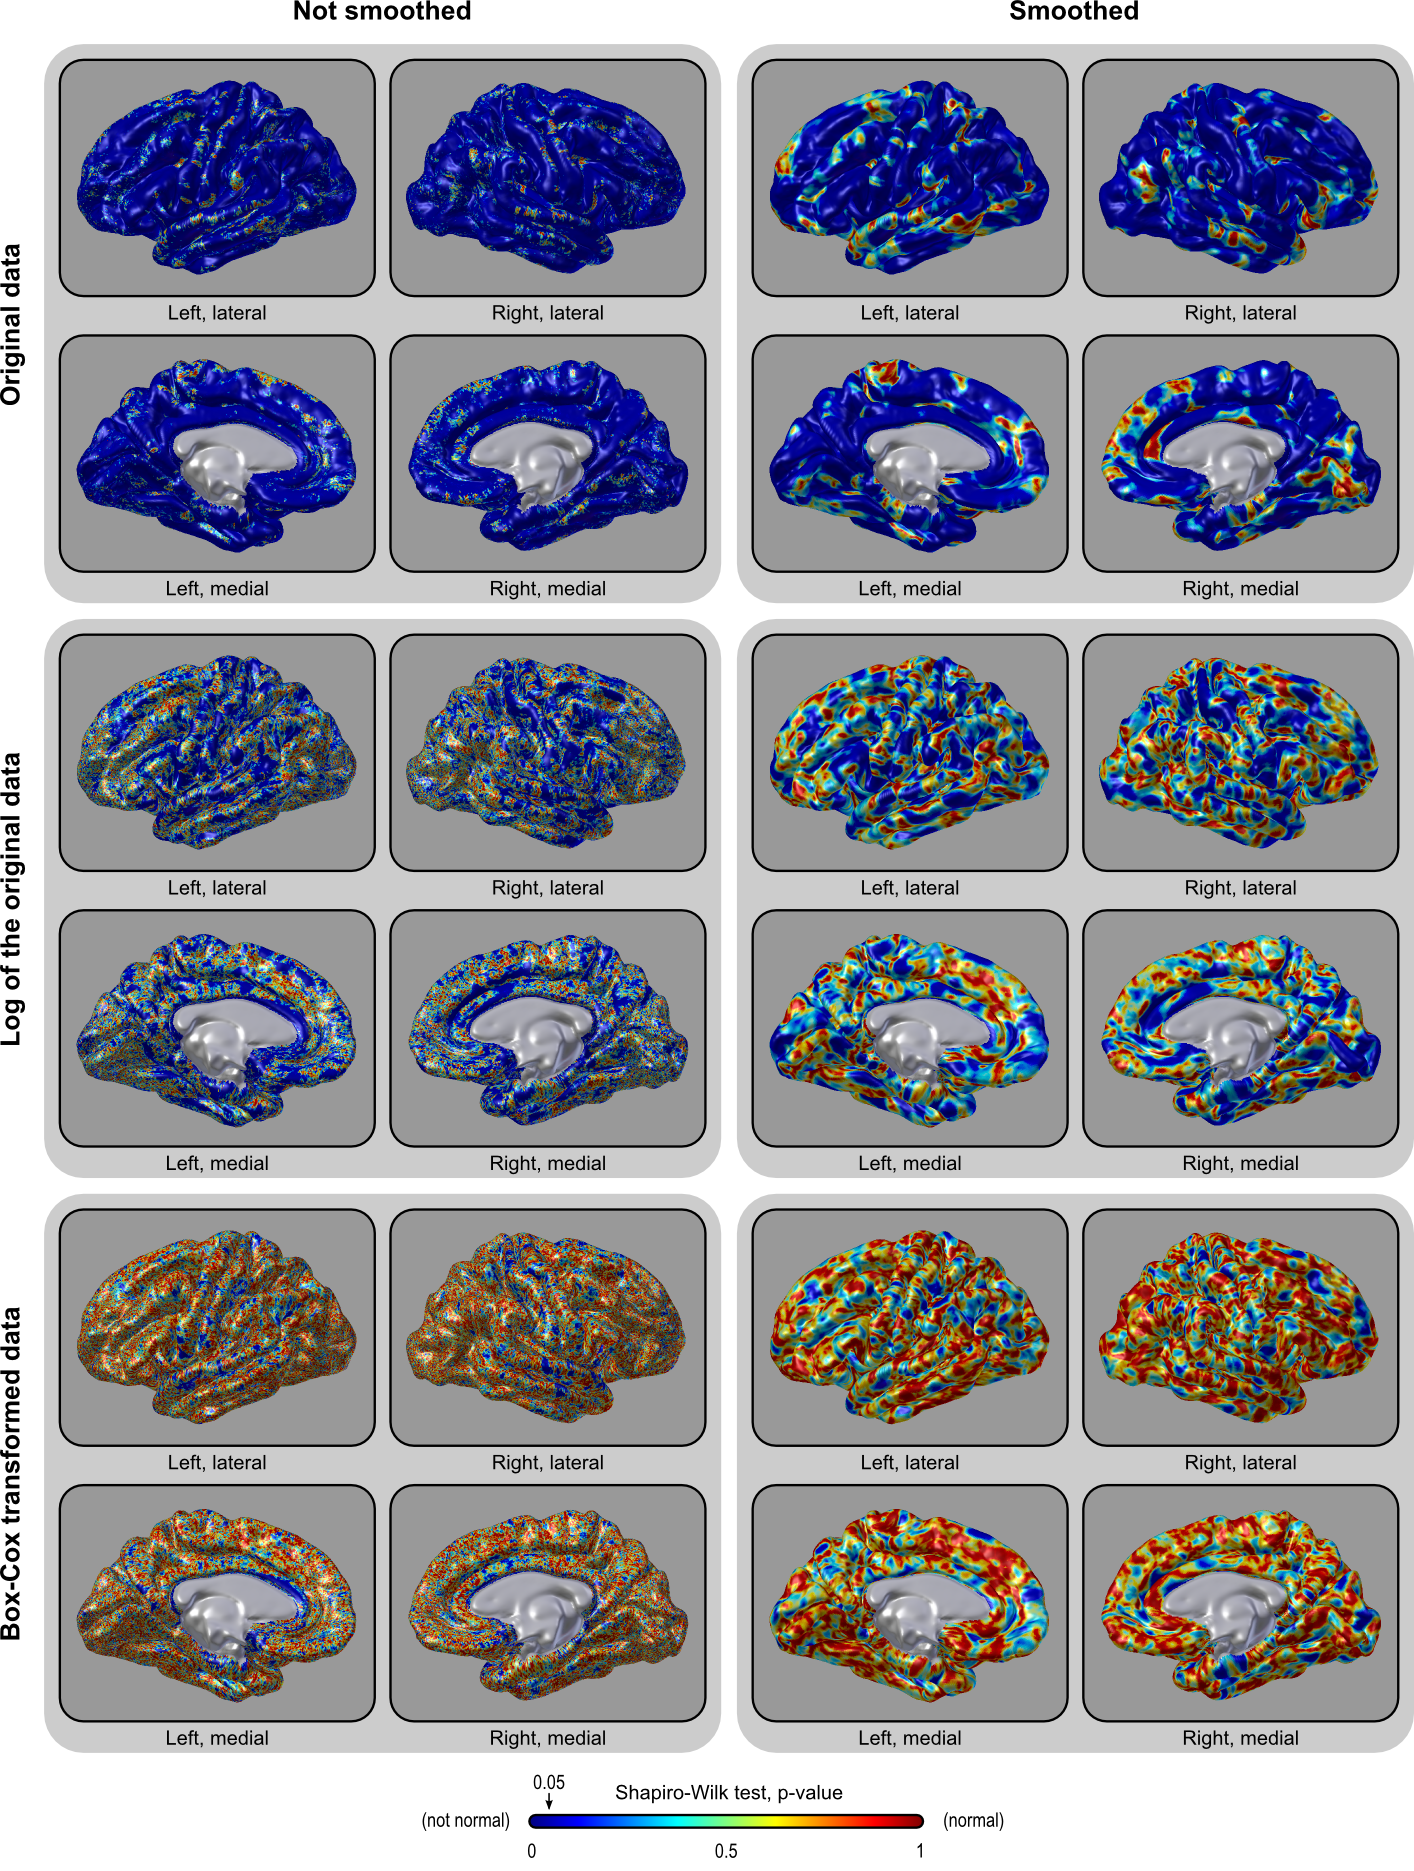
\includegraphics[width=14cm]{images/shapiro.png}
\caption[The distribution of surface area is lognormal.]{The area of the cortical surface is not normally distributed (upper panels). Instead, it is lognormally distributed throughout most of the brain (middle panels). A Box--Cox transformation can further improve normality (lower panels). The same pattern is present without (left) or with (right) smoothing (\textsc{fwhm} = 10~mm). Although normality is not an assumption for inference as proposed, it offers some advantages, as discussed in the text.}
\label{fig:shapiro}
\end{figure}

\begin{figure}[!p]  % Figure 6
\centering
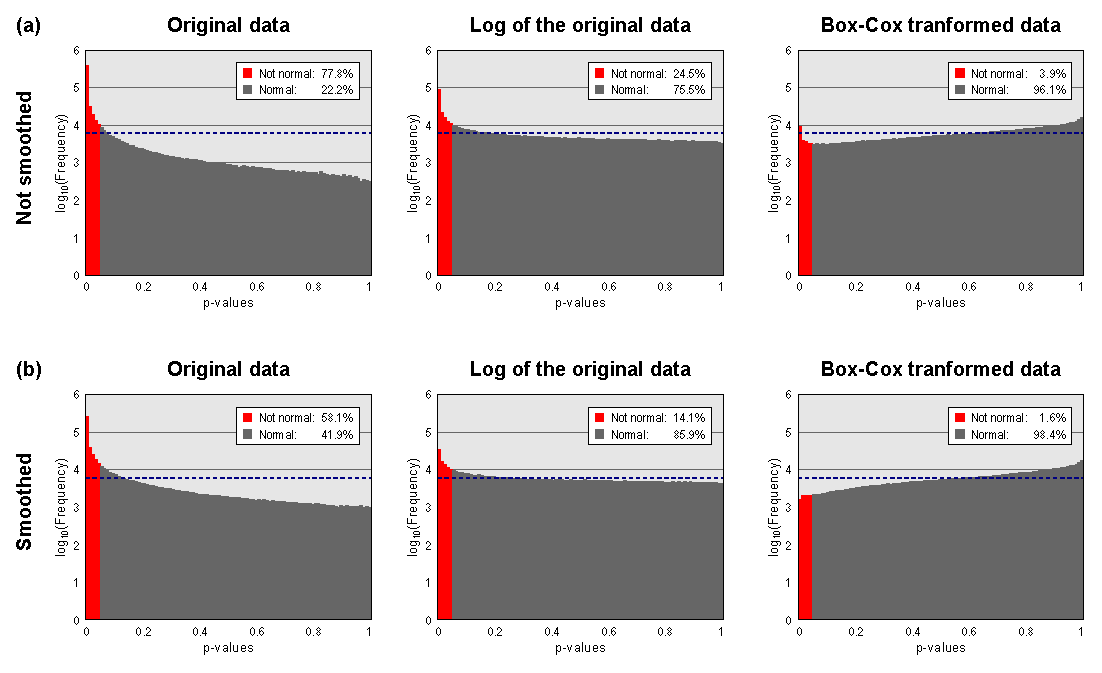
\includegraphics[width=14cm]{images/histograms.eps}
\caption[Results of the Shapiro--Wilk normality test.]{Distribution of the uncorrected p-values of the Shapiro--Wilk normality test. For normally distributed data, 5\% of these tests are always expected to be declared as not normal with a significance level of $\mathsf{\alpha=0.05}$. Without transformation or smoothing, near 80\% are found as not normal. Logarithmic and Box--Cox transformations render the data more normally distributed. Observe that the frequencies are shown in logscale. The dashed line (blue) is at the frequency that would be observed for uniformly distributed p-values.}
\label{fig:histograms}
\end{figure}

\begin{figure}[!p]  % Figure Suppl 3
\centering
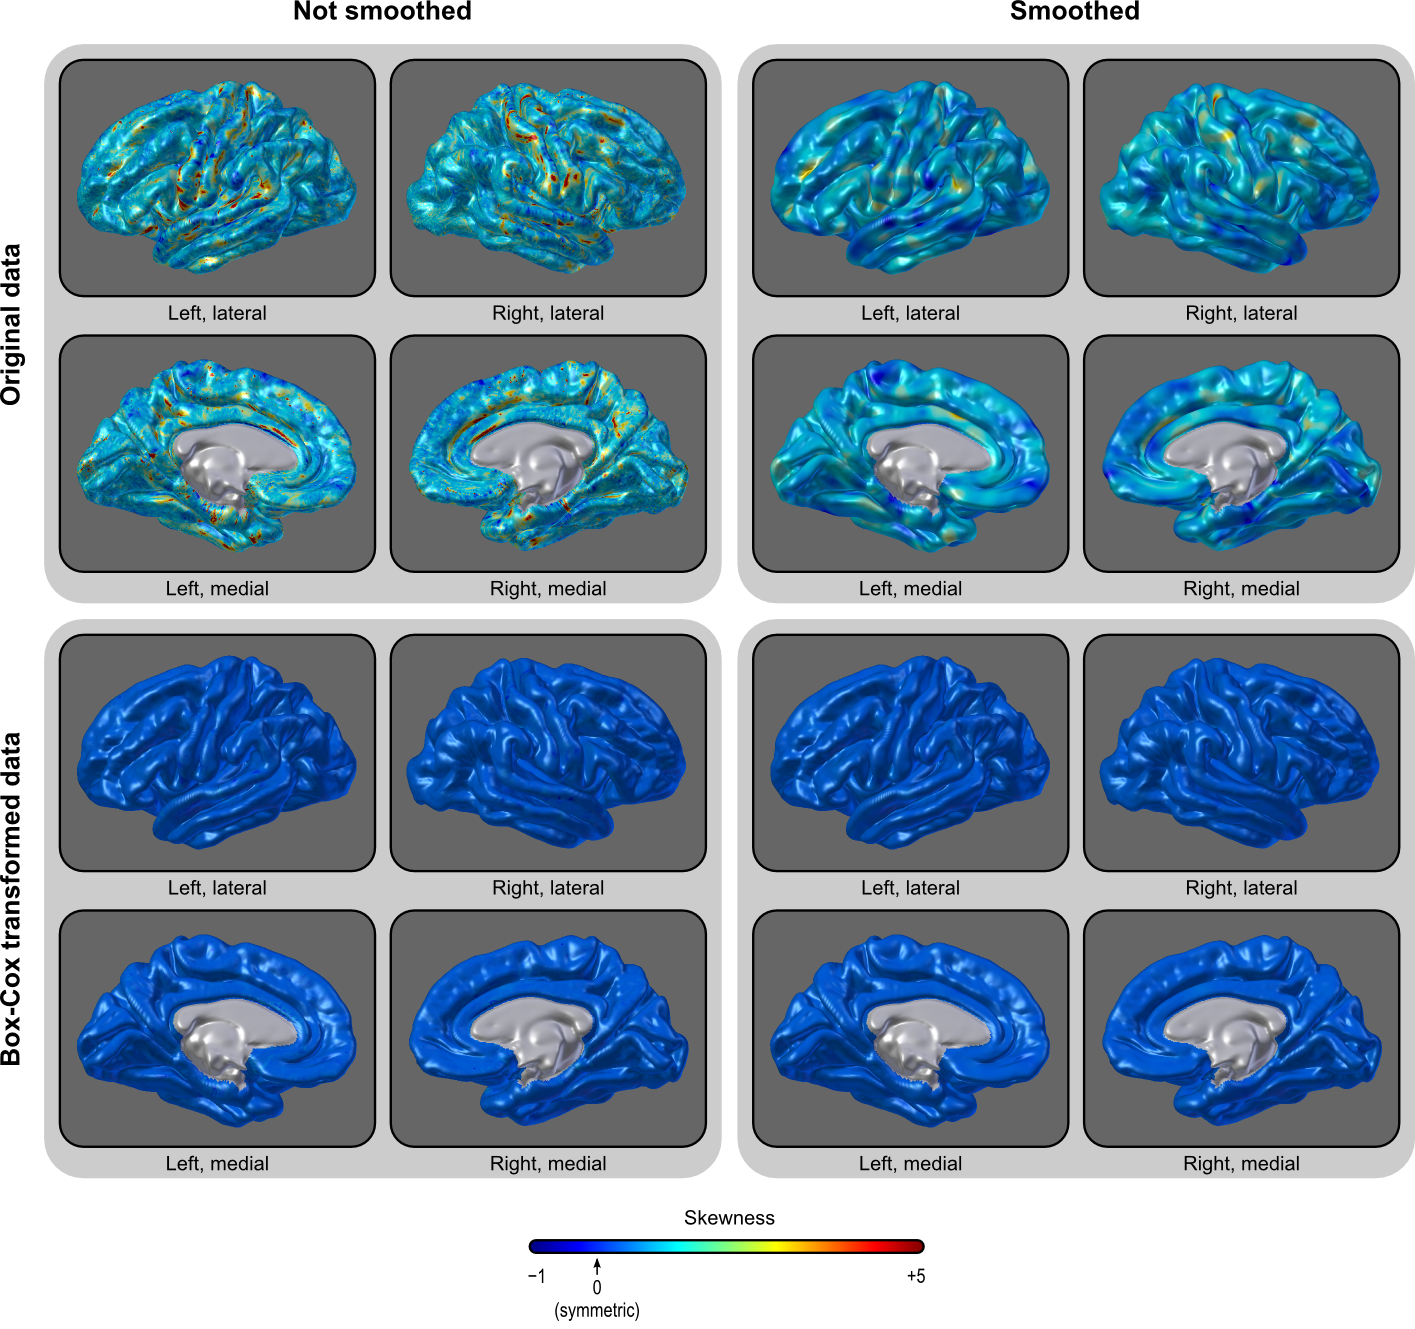
\includegraphics[width=14cm]{images/skewness.png}
\caption[Maps of the skewness of the areal data.]{Maps of the skewness of the areal data, before and after the Box--Cox transformation, and with and without smoothing. The distribution is positively skewed (lognormal) throughout most of the brain, and the transformation successfully brings the data to symmetry (normality). The histograms are shown in Supplemental Figure \ref{fig:skewness-hist}.}
\label{fig:skewness}
\end{figure}

\begin{figure}[!p]  % Figure Suppl 4
\centering
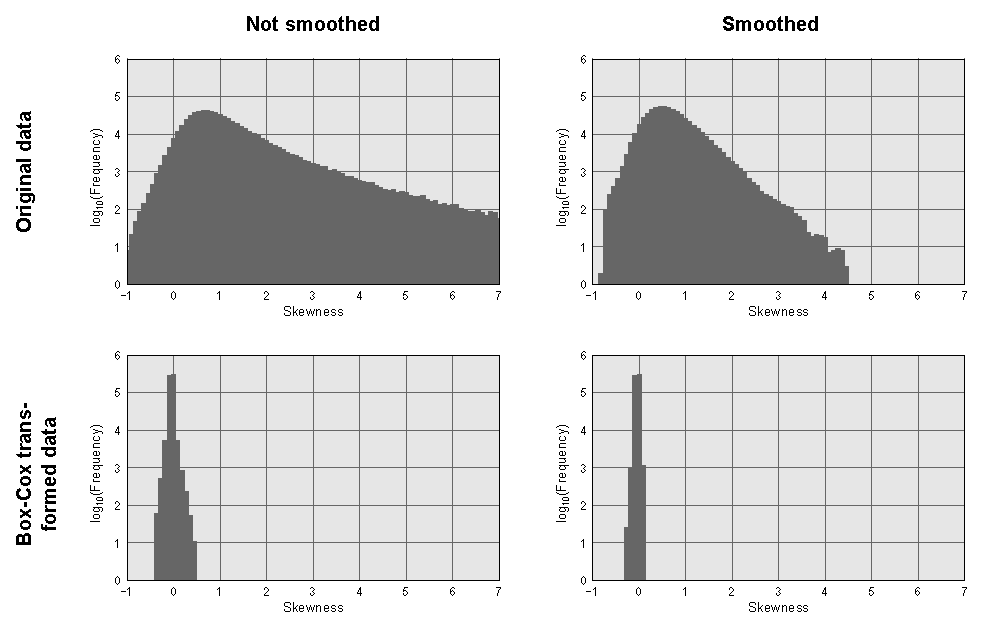
\includegraphics[width=14cm]{images/skewness-hist.eps}
\caption[Histograms of the skewness of the areal data.]{Histograms of the skewness of the areal data, before and after the Box--Cox transformation, and with and without smoothing. The distribution is positively skewed (lognormal) throughout most of the brain, and the transformation successfully brings the data to symmetry (normality). Note that the frequencies are shown in log scale. The corresponding maps are in Supplemental Figure \ref{fig:skewness}.}
\label{fig:skewness-hist}
\end{figure}

\begin{figure}[!p]  % Figure Suppl 5
\centering
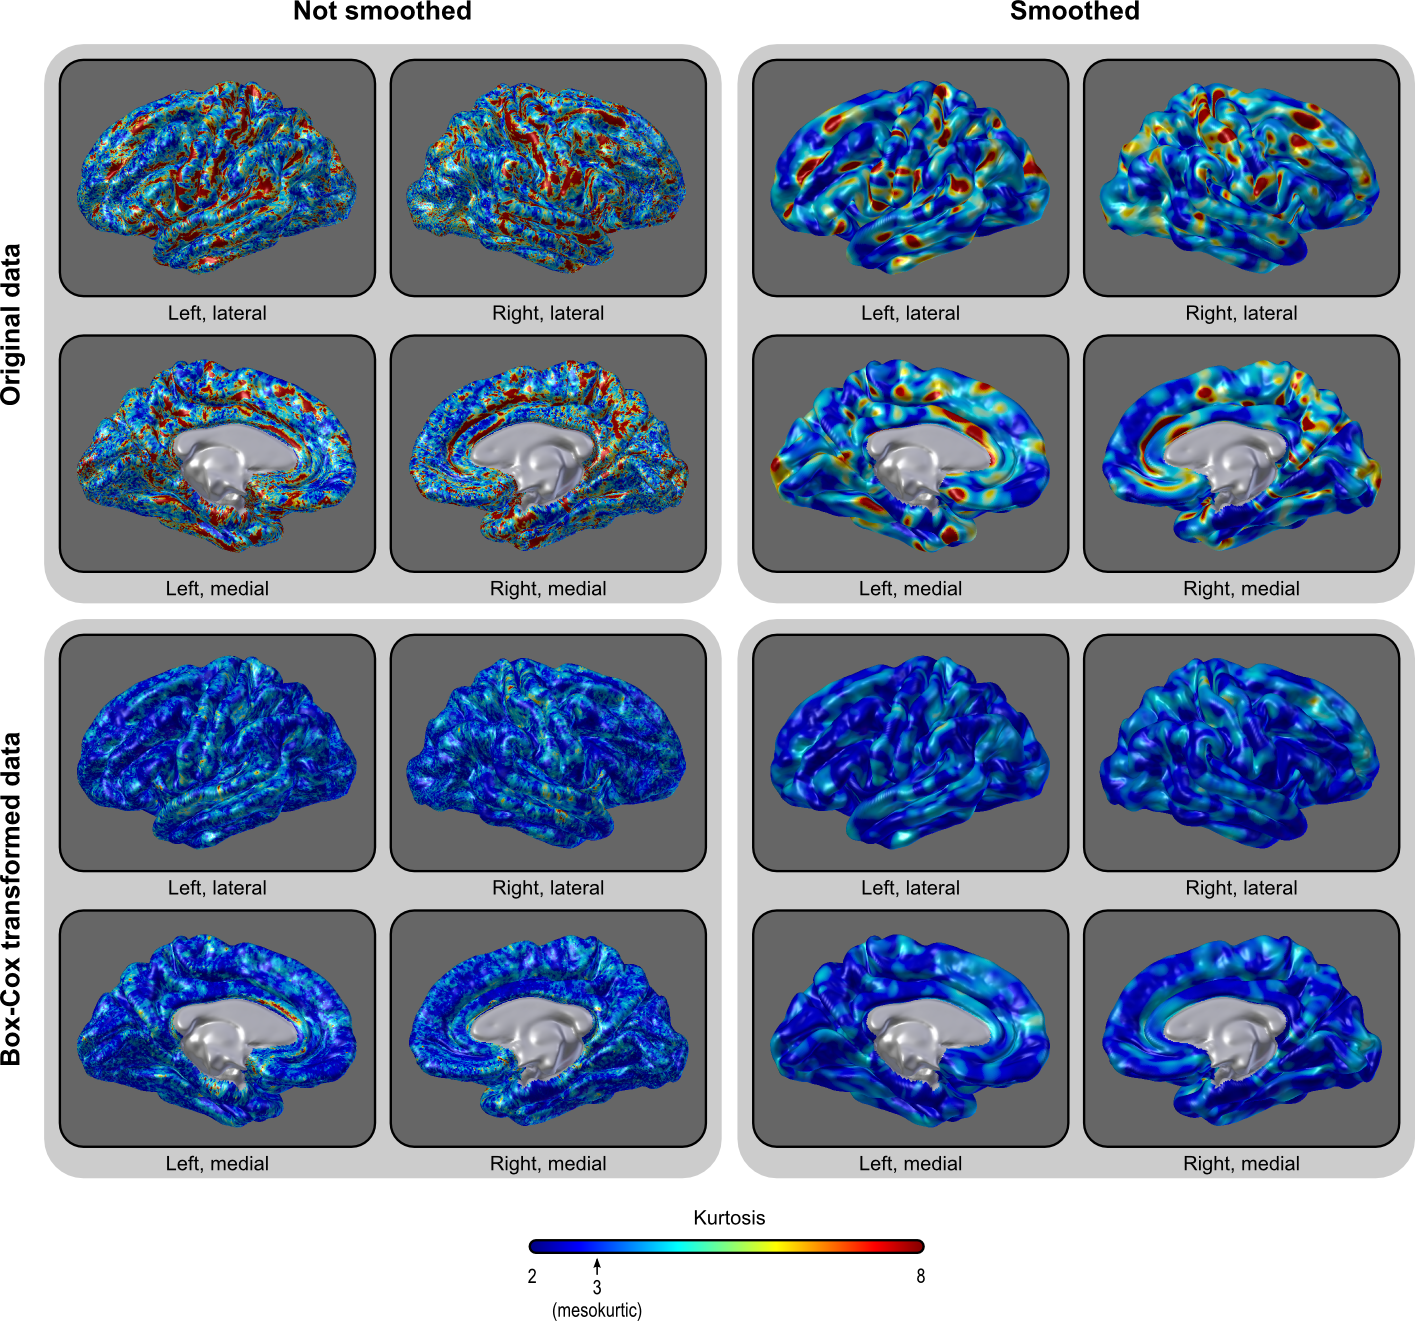
\includegraphics[width=14cm]{images/kurtosis.png}
\caption[Maps of the kurtosis of the areal data.]{Maps of the kurtosis of the areal data, before and after the Box--Cox transformation, and with and without smoothing. The distribution is leptokurtic throughout most of the brain, and the transformation renders the kurtosis closer to the same value as for the normal distribution, i.e.\ closer to the value 3. The histograms are shown in Supplemental Figure \ref{fig:kurtosis-hist}.}
\label{fig:kurtosis}
\end{figure}

\begin{figure}[!p]  % Figure Suppl 6
\centering
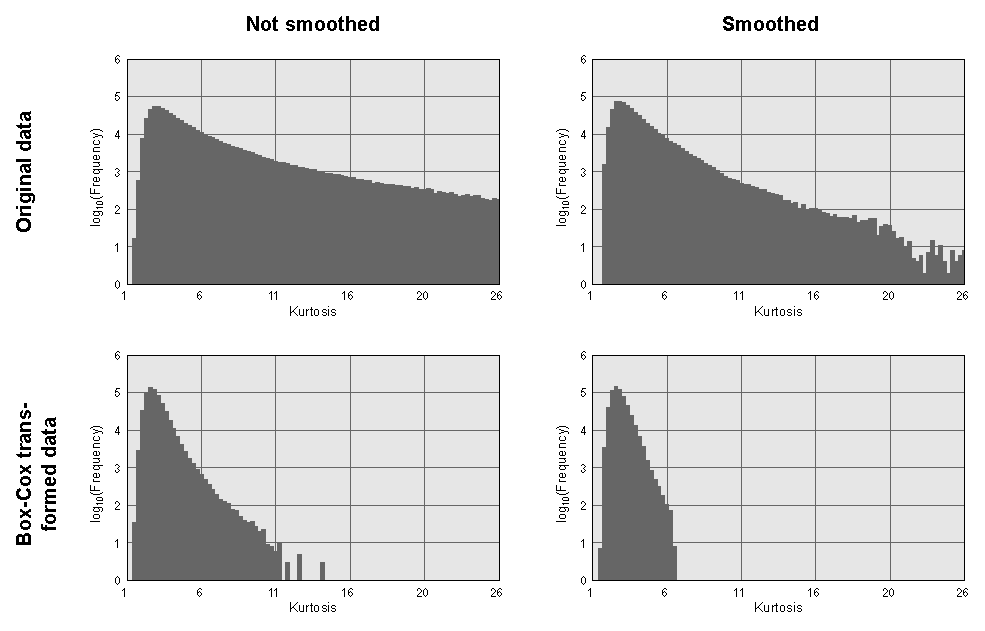
\includegraphics[width=14cm]{images/kurtosis-hist.eps}
\caption[Histograms of the kurtosis of the areal data.]{Histograms of the kurtosis of the areal data, before and after the Box--Cox transformation, and with and without smoothing. The distribution is leptokurtic throughout most of the brain, and the transformation renders the kurtosis closer to the same value as for the normal distribution, i.e.\ closer to the value 3.  Note that the frequencies are shown in log scale. The corresponding maps are in Supplemental Figure \ref{fig:kurtosis}.}
\label{fig:kurtosis-hist}
\end{figure}

\begin{figure}[!p]  % Figure Suppl 2
\centering
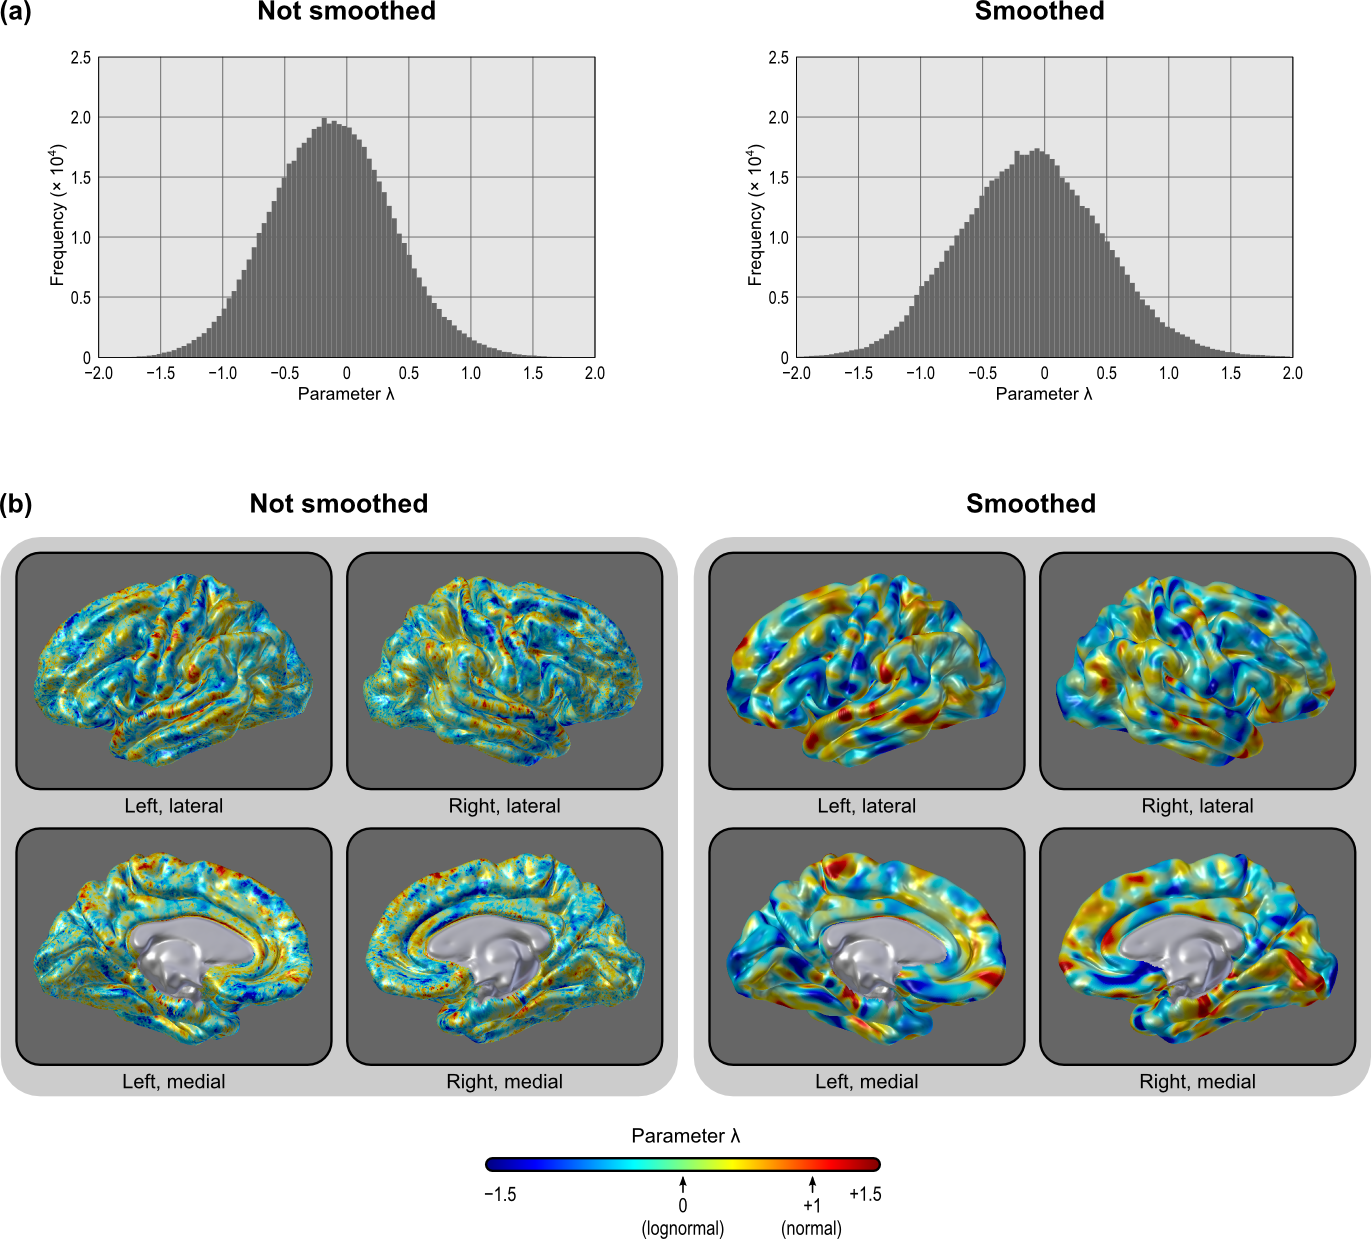
\includegraphics[width=14cm]{images/boxcox.png}
\caption[Spatial distribution of the parameter $\lambda$.]{Distribution of the parameter $\lambda$ of the Box--Cox transformation across the brain: (a) histogram and (b) spatial map. When $\lambda$ approaches zero, the distribution of the underlying data is more lognormal.}
\label{fig:boxcox}
\end{figure}

\subsection{Comparison with expansion/contraction methods}

A number of studies have analysed what has been called expansion or contraction of the cortical surface when compared to a reference brain. Different studies adopted different operational definitions for what these terms would be [e.g.\ compare \citet{Joyner2009}, \citet{Sun2009}, \citet{Hill2010}], and an unified approach has not been defined. Notwithstanding, the key difference between these methods and the proposed areal analysis is that, at the end of the processing pipeline, areal interpolation ensures the preservation of the amount (mass) of quantities, whereas these methods do not. Moreover, in the framework we present, a number of potential problems that may arise along the pipeline are explicitly addressed. These problems, along with the solutions we propose, are summarized in Table~\ref{tab:compare}.

\begin{table}[!p]
\caption[Problems solved by the proposed method.]{The proposed framework for areal analyses addresses a number of potential problems that may arise along the processing pipeline.}
\begin{center}
{\small
\begin{tabular}{@{}m{42mm}<{\raggedright}m{44mm}<{\raggedright}m{43mm}<{\raggedright}@{}}
\toprule
\textbf{Processing step} &
\textbf{Problem} &
\textbf{Solution} \\
\midrule
Measurements assigned to vertices at the beginning of the analysis. &
Vertices do not hold or convey the same spatial information as the original faces. &
Analyze the faces directly. \\
\midrule
Registration methods that not necessarily produce smooth and invertible warps. &
Discontinuities on expansion or contraction that are not present in the actual brain. &
Use diffeomorphic registration methods. \\
\midrule
Interpolation based on points. &
Areal quantities are not preserved at any scale (local, regional or global). &
Use areal interpolation. \\
\midrule
Use of a standard brain to compute the same measurement that is later analysed. &
Results are interpretable only with respect to that same reference brain. &
Measure and analyse absolute quantities, not relative to some reference. \\
\midrule
Statistical analysis based on assumption of normality. &
The local surface area follows a lognormal distribution. &
Apply a data transformation. Use non-parametric methods. \\
\bottomrule
\end{tabular}}
\end{center}
\label{tab:compare}
\end{table}

With a variety of expansion/contraction methods available, it is difficult to identify the best to which areal analysis could be compared. Here we retessellate the each subject brain in native space using the method described by \citet{Saad2004}. The expansion/contraction method was implemented using the following steps: (1) From the native surface geometry, perform the spherical transformation; (2) Perform the spherical registration to a standard brain; (3) Treat the coordinates $x$, $y$ and $z$ of the vertices from the native geometry as three independent scalar fields over the registed sphere, and interpolate these values to the common spherical grid using barycentric interpolation\footnote{The three scalar fields can also be treated as a single vector field and the barycentric interpolation can be performed in a single step as
\begin{displaymath}
\left[
\begin{array}{c}
x_{P} \\
y_{P} \\
z_{P}
\end{array} \right] = \left[
\begin{array}{ccc}
x_{A} & x_{B} & x_{C} \\
y_{A} & y_{B} & y_{C} \\
z_{A} & z_{B} & z_{C} \\
\end{array}
\right] \left[
\begin{array}{c}
\delta_{A} \\
\delta_{B} \\
\delta_{C}
\end{array} \right]
\end{displaymath} where $x,y,z$ represent the coordinates of the triangular face $ABC$ and of the interpolated point $P$, both in native geometry, and $\delta$ are the barycentric coordinates of $P$ with respect to the same face after the spherical transformation.}; (4) Use the interpolated coordinates, together with the same connectivity scheme between vertices as in the common grid, to construct a new model of the brain in a subject-specific geometry (Figure~\ref{fig:retessellate}); (5) From this new model, compute the area per vertex and divide it by the area per vertex of the homologous point in the template. Call this measurement \emph{expansion/contraction}; (6) Optionally, smooth this quantity.

\begin{figure}[!tbp]  % Figure 7
\centering
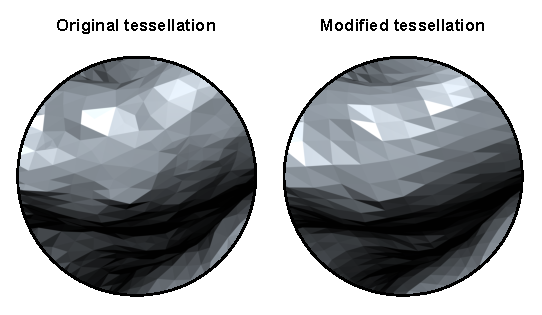
\includegraphics[width=10cm]{images/retessellate.eps}
\caption[Example of a retessellated surface.]{After barycentric interpolation of the coordinates in the surface of the sphere, a new, subject-specific retessellated model is constructed. Areas can be computed directly from the retessellated model and, once divided by the areas of the homologous vertices or faces of the reference brain, constitute the measurement of expansion/contraction.}
\label{fig:retessellate}
\end{figure}

For comparison with the expansion/contraction method, the original facewise area was converted to vertexwise, therefore halving the spatial resolution of the areal data (see Appendix~\ref{sec:conversion}). In this comparison, we addressed some of the problems presented in Table~\ref{tab:compare}, namely, we registered using Spherical Demons, therefore ensuring smooth and invertible warps, and as target for registration, we used the study-specific template that produced the best results in Figure~\ref{fig:registration}. Furthermore, the measurements were taken at the white surface, rather than the middle surface, as the last is more prone to be influenced by the cortical thickness. It is unclear if, when applicable, these aspects were taken care of in all the different studies that analysed some form of expansion/contraction.

After establishing an expansion/contraction procedure, there are still different ways to compare with areal analysis. The comparison can be made across subjects or across space, can be global or regional, and may or may not include smoothing. In Figure~\ref{fig:expansion} we show that the average amount of area at each vertex did not produce a similar spatial map as the average expansion/contraction. Although the two methods follow remarkably different overall spatial patterns, when vertices across space were pooled together to produce a global measurement, they produced very similar results. Figure~\ref{fig:scatter}a shows the relationship between the global cortical surface area, computed from the sum of the area at each vertex, and a global measure of expansion computed by averaging the expansion/contraction at each vertex across space.\footnote{Note that an exact measurement of expansion/contraction relative to the template can be produced simply by dividing the global area in native geometry by the area of the template geometry. In this case, the points in Figure~\ref{fig:scatter}a would lie in a perfectly straight line, and nothing could be inferred about the relationship between regional variability on expansion estimates and global measurements.} The correlation was very high and helps to validate both methods as a whole. Likewise, when each vertex was analysed separately, the correlation across subjects was also very high, as shown in Figure~\ref{fig:spatialfit}, with an $R^2$ above 0.9 throughout virtually the whole cortex. A spatial comparison of the average maps, on the other hand, showed a very poor relationship between both approaches, as shown in Figure~\ref{fig:scatter}b. When looking at each individual subject, rather than at the average, the correlation across space was still relatively low, albeit not as poor: for the 168 hemispheres analysed, we found an average linear $R^2=0.572$, $\text{sd}=0.044$ without smoothing, and $R^2=0.491$, $\text{sd}=0.065$ after smoothing.

\begin{figure}[!tp]  % Figure 8
\centering
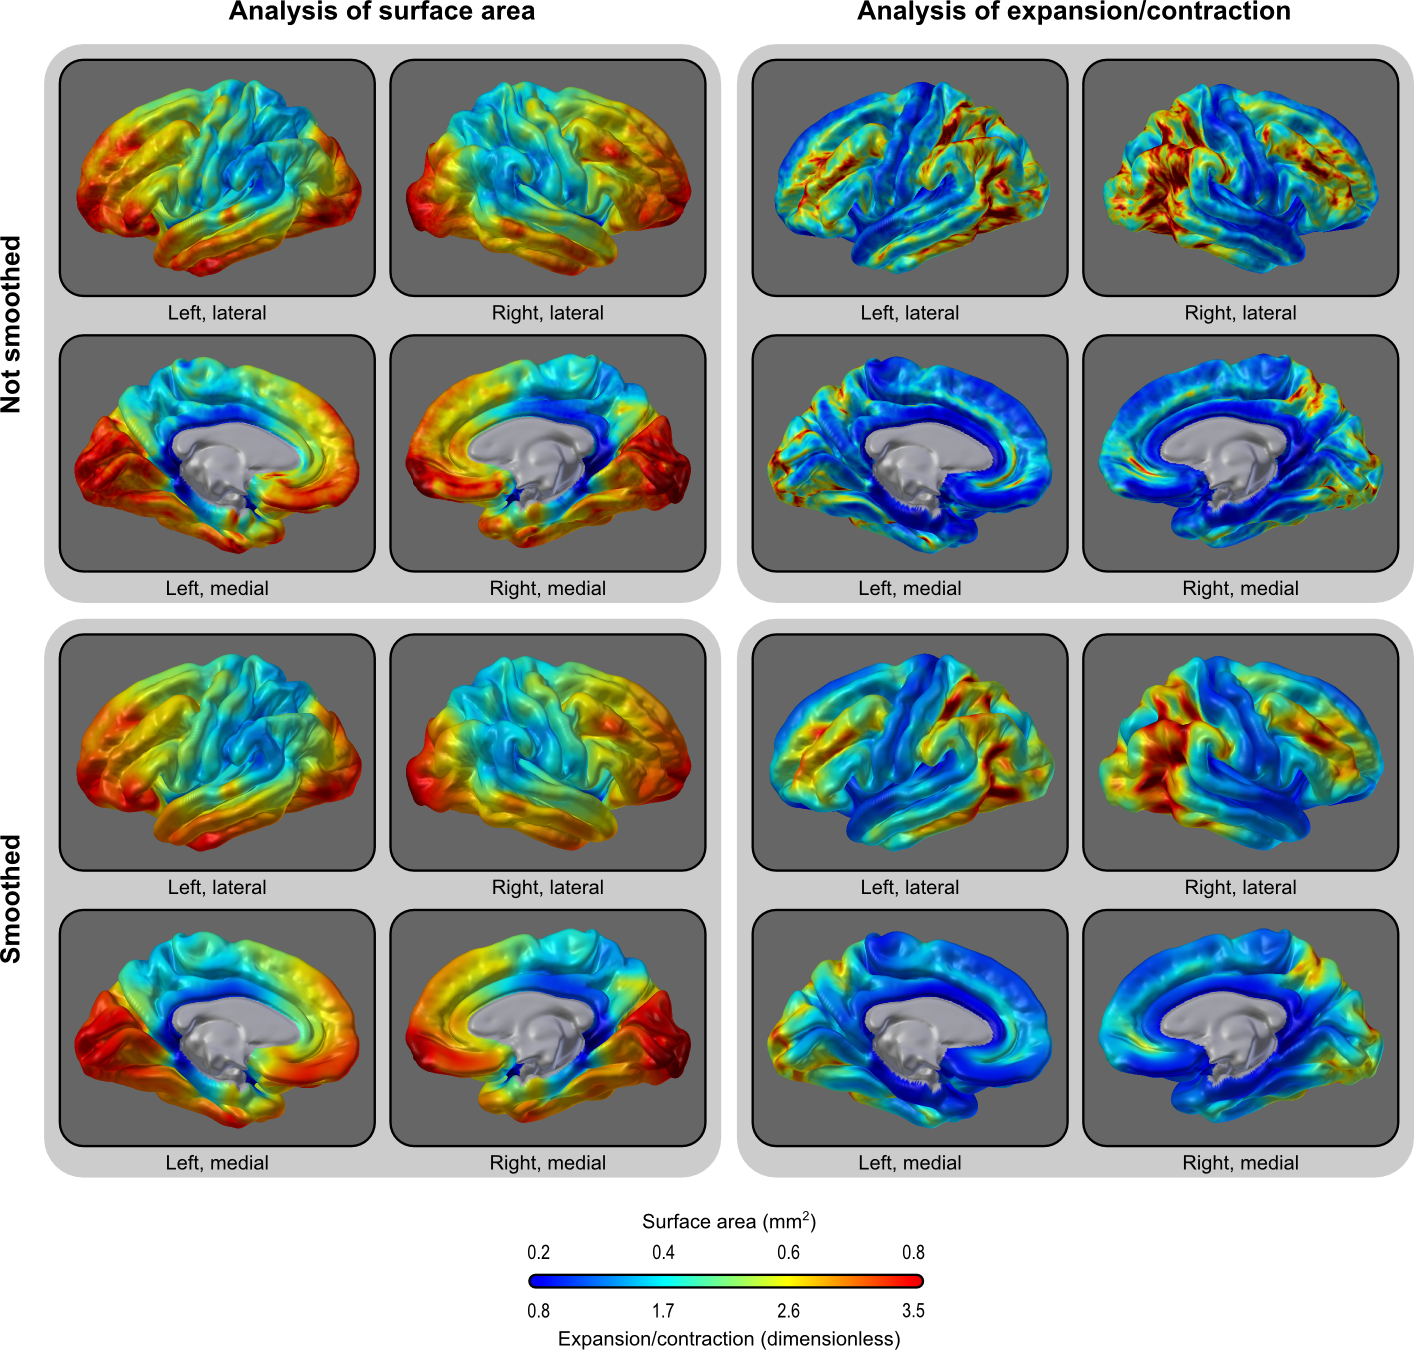
\includegraphics[width=14cm]{images/expansion.png}
\caption[Comparison with expansion/contraction methods (\textsc{i}).]{Average area (left panels) or expansion/contraction (right panels) per vertex, without (upper panels) and with smoothing (lower panels). Areal analyses and expansion/contraction differ across space. Smoothing has little global impact.}
\label{fig:expansion}
\end{figure}

\begin{figure}[!tp]  % Figure 9
\centering
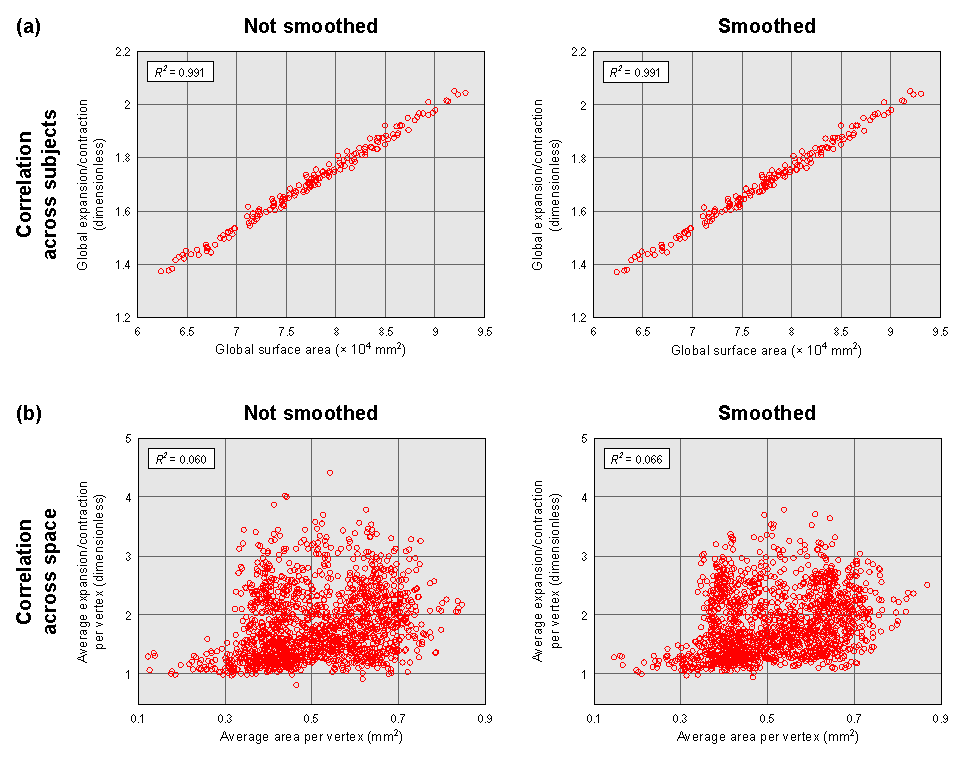
\includegraphics[width=14cm]{images/scatter.eps}
\caption[Comparison with expansion/contraction methods (\textsc{ii}).]{(a) The sum of the area per vertex correlates well with the average across space of the expansion/contraction at each vertex (i.e. equivalent to a weighed sum considering each vertex as having the same initial area) for the 168 hemispheres analysed. For the expansion/contraction, this is not the same as computing the ratio between the global surface area in native geometry and of the template, in which case, the result would be a perfectly straight line. The high correlation implies that the regional differences in general compensate each other to produce a similar global effect. (b) The correlation between average spatial maps across the 84 subjects, both hemispheres, is very poor between the methods. [Note that, for (b), attempts to simultaneously plot all the $>$~300 thousand vertices would not produce meaningful plots in a small space; for this reason only 5\% of the vertices were randomly selected for plotting. The $R^2$ were computed from all vertices and, for both (a) and (b), the value corresponds to the goodness of a linear fit.]}
\label{fig:scatter}
\end{figure}

\begin{figure}[!tp]  % Figure 10
\centering
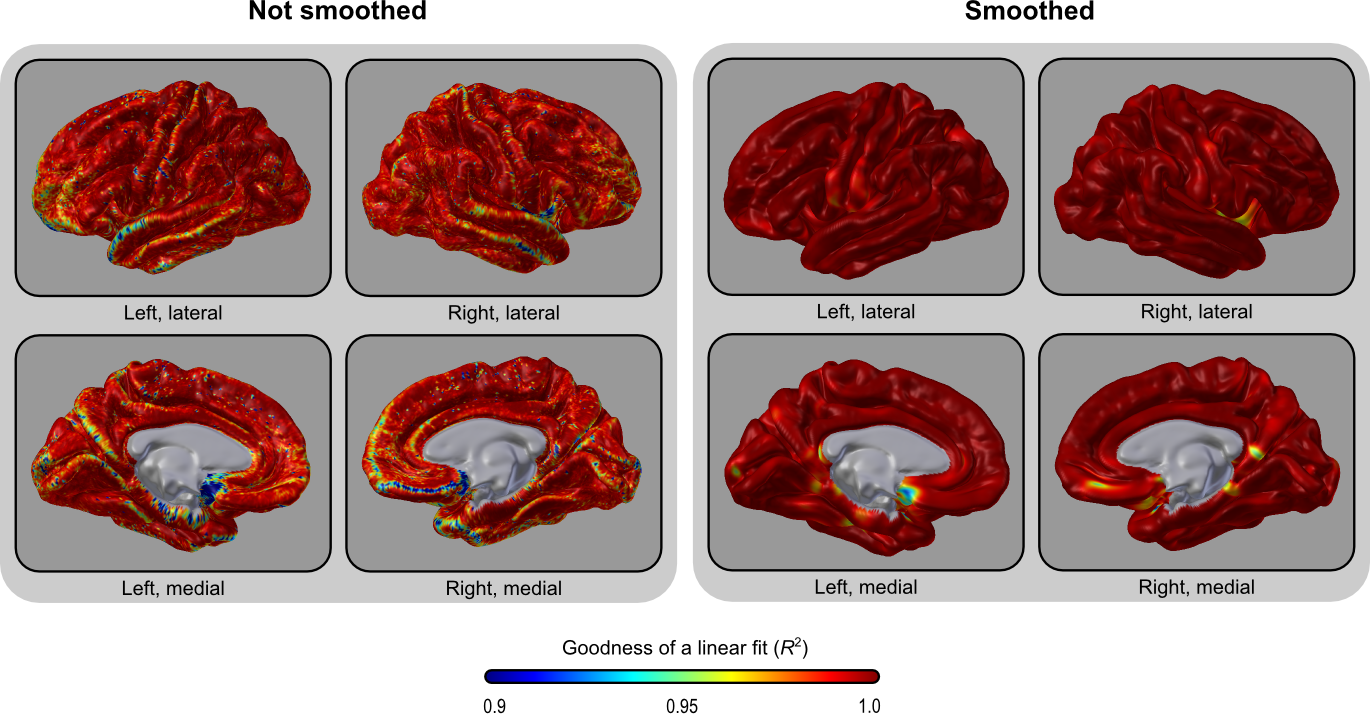
\includegraphics[width=14cm]{images/spatialfit.png}
\caption[Comparison with expansion/contraction methods (\textsc{iii}).]{For each vertex, the linear relationship between areal analyses and expansion/contraction is very high across subjects, being above $R^2=$~0.90 virtually across the whole cortex.}
\label{fig:spatialfit}
\end{figure}

These results suggest that, if each vertex is analysed in isolation, analysis of surface area and analysis of expansion/contraction tend to produce similar results. This is the case, for instance, using mass univariate \textsc{glm}-based approaches. However, for analysis that involve spatial information or that combine information across neighboring vertices, the results are expected to be rather dissimilar. The difference stems from the different units of measurement: areal analyses produce measurements in absolute units of area (e.g.\ mm$^2$), whereas expansion/contraction are relative to the a given reference. The result shown in Figure~\ref{fig:spatialfit}, left panel, also demonstrate, indirectly, that areas measured in the retessellated brain with the resolution used correlate reasonably well with the areas obtained using areal interpolation, and so, have potential to be used as a fast approximation to areal interpolation (Appendix~\ref{sec:implementation}). Conversely, expansion/contraction measurements can be obtained after areal interpolation simply by dividing the area per face (or per vertex) by its homologous in the reference brain.

\subsection{Validation and stability}

Measurements of surface area are valid as long as the surface reconstruction from \textsc{mr} images produces accurate representations of the cortex. The suggested reconstruction method has been previously validated \citep{Fischl2000}, and is widely used for cortical thickness measurements. Comparison between subjects at the face level depends on good matching of homologies and the registration method we suggest has, likewise, been previously validated \citep{Yeo2010, Klein2010}. As methods evolve, novel approaches for constructing surface representations of the cortex and for registration have potential to improve the overall quality of areal analyses. The validity of areal measurements other than surface area itself depend on each particular measurement technique.

To assess the stability across sessions and scanners, we compared \textsc{mr} images of the same subject acquired in three different sessions collected within a 1 year interval. The imaging protocol varied in terms of acquisition parameters, as well as the number of images used for averaging and improvements on signal and contrast-to-noise ratio. The details are summarized in Table~\ref{tab:retest}. The estimated surface area produced by summing the facewise areas over the cortex after interpolation was very similar across tests, with the largest difference being 8.2\% between Tests \textsc{a} and \textsc{c} (see Table~\ref{tab:retest}), with or without smoothing. The mean and standard deviation for facewise areas were virtually identical across tests, again regardless of smoothing. The pairwise Pearson correlation between the tests for the facewise data after registration and interpolation was above 0.80 without smoothing, and above 0.90 after smoothing with \textsc{fwhm} = 10~mm, showing that the procedure is robust at the face level, even under different scanning conditions and degrees of smoothing.

\begin{table}[!tp]
\caption[Stability of areal measurements.]{Stability and robustness of measurements after registration and interpolation were assessed using three test images of the same subject. The measurements were similar across tests, with similar variability across space and high spatial correlation.}
\begin{center}
{\footnotesize
\begin{tabular}{@{}l@{}m{33mm}<{\centering}@{}m{33mm}<{\centering}@{}m{33mm}<{\centering}@{}}
\toprule
{} & \textbf{Test A} & \textbf{Test B} & \textbf{Test C}\\
\midrule
Manufacturer and model & Siemens~\textsc{magnetom} Trio~3~T & Siemens~\textsc{magnetom} Trio/\textsc{tim}~3~T & Siemens~\textsc{magnetom} Allegra~3~T \\
Sequence & \textsc{mprage} & \textsc{mprage} & \textsc{mprage} \\
\textsc{te/ti/tr} (ms) & 3.04/785/2100 & 2.83/766/2200 & 2.74/900/2500 \\
Flip angle & 13$^{\circ}$ & 13$^{\circ}$ & 8$^{\circ}$ \\
Voxel size (mm) & $0.8 \times 0.8 \times 0.8$ & $0.8 \times 0.8 \times 0.8$ & $1.0 \times 1.0 \times 1.0$ \\
Number of acquisitions & 14 & 7 & 1 \\
Scan date & March 2008 & March 2008 & April 2009 \\
Cortical surface area (mm$^2$) & 176,996 & 177,098 & 180,949 \\
\midrule
\multicolumn{4}{l}{\textbf{Not smoothed}}\\
Average area per face (mm$^2$) & 0.2937 & 0.2939 & 0.3003 \\
Standard deviation             & 0.0938 & 0.0910 & 0.0962 \\
Correlation with Test A        &    --- & 0.8218 & 0.7589 \\
Correlation with Test B        & 0.8218 &    --- & 0.7863 \\
Correlation with Test C        & 0.7589 & 0.7863 &    --- \\
\midrule
\multicolumn{4}{l}{\textbf{Smoothed (\textsc{fwhm} = 10~mm)}}\\
Average area per face (mm$^2$) & 0.2935 & 0.2936 & 0.3000 \\
Standard deviation             & 0.0746 & 0.0712 & 0.0748 \\
Correlation with Test A        &    --- & 0.9509 & 0.9074 \\
Correlation with Test B        & 0.9509 &    --- & 0.9353 \\
Correlation with Test C        & 0.9047 & 0.9353 &    --- \\
\bottomrule
\end{tabular}}
\end{center}
\label{tab:retest}
\end{table}

\section{Discussion}

\subsection{Registration}

To be valid, facewise analyses rely on the assumption that microscopic structures can be localized using as reference the features that are identifiable with \textsc{mri} and which drive the registration. Features with such localizing power are important because they help to ensure good overlap of homologous areas between subjects. Despite an implicit assumption already present in most imaging studies, only recently it has been demonstrated valid for some cytoarchitetonic areas when the references are the cortical folding patterns, even though for non-primary regions, the mismatch may still be substantial \citep{Fischl2008, Fischl2009, Hinds2008, Hinds2009, DaCosta2011}. Other features, some microscopic and detectable only under ultra-high field strengths \citep{Augustinack2005, Bridge2006, Duyn2007, Kim2009}, have the potential to be used as the reference as long as they are demonstrated to be markers of histologically or functionally defined areas, possibly replacing folding patterns altogether, or used to provide ancillary information. Myeloarchitectural features may be particularly useful for this application, for being resposible for most of the contrast observed with \textsc{mri} \citep{Geyer2011}. Likewise, areal analyses can be conducted after registration based on features derived from functional \textsc{mri} \citep{Sabuncu2010}.

Good matching of homologies, however, depends not only on the features used to guide the registration, but on the registration method itself. For facewise areal analyses, invertibility is necessary to prevent faces from being folded over others. In addition, methods that produce smooth warps are necessary to ensure that areal quantities are transferred smoothly, without abrupt variations. Such abrupt variations would only be acceptable if matching perfectly with areas where structure and/or function also changes abruptly. A spatial transformation that allows such perfect matching, however, cannot be obtained easily in practice, since these borders usually cannot be observed with current, conventional \textsc{mri} methods, and importantly, since many of the differences between regions are subtle and the transitions are gradual. However, invertibility and smoothness, as guaranteed by diffeomorphic methods, albeit important, may not suffice. Our results show that even methods that produce smooth varying warps can differ substantially with respect to how the areal quantities are shifted across the surface. It is possible that performance differences between these methods might be due to choices on regularization strategies and associated parameters \citep{Fischl1999_intersubject, Yeo2010}, instigating further reseach on selections that may produce the most accurate results \citep{Yeo2010b}. Our experiments also demonstrate that the choice of the target used for registration affects the distortion in areal measurements.

\subsection{Areal interpolation}

Areal interpolation allows direct analysis of areal quantities in absolute values, including the surface area itself. This is because it is the areal quantity proper that is conservatively transfered between grids. Therefore, there is no need to apply corrections due to stretches or shrinkages, such as using the Jacobian of the transformation \citep{Good2001}, nor due to the choice of the parametrizable surface \citep{Thompson1999}. Moreover, the results are interpretable directly with regard to the actual amount of tissue or other measurement under study, rather than relative to concepts as expansion/contraction, which are always relative to a given reference, and can create difficulties in interpretation and comparison across studies, either due to different definitions adopted by different authors, or due to the the need of a reference brain. Notwithstanding, after areal interpolation, it continues to be possible to divide the areas by the areas of the homologous faces or vertices of a reference brain, and so, obtain an expansion/contraction measurement. Moreover, areal quantities that are not area itself can also be divided by the area of each face or vertex in native geometry, thus converting these quantities to densities if necessary.

It should be emphasized that, as with other interpolation strategies, areal interpolation is not perfectly reversible, i.e.\ once the cortical area of a subject is transferred to a different grid, remapping back to the subject surface will not produce locally identical results, although the global areal quantity is always conserved. This is because within each face, the areal quantity is implicitly assumed to be homogeneously distributed. This only becomes a problem if low resolution meshes are used and if several back-and-forth iterations are performed.

\subsection{Statistical analysis of areal quantities}

There are a number of reasons that go beyond purely methodological considerations to justify the transformation of the data before statistical analysis. Measurements related to biological morphology, such as lengths, areas, volumes or weights, are well known to follow non-normal distributions. If the diameter of a structure, for instance, is normally distributed, inevitably both its cross section and its surface area follow skewed distributions, whereas its volume follows an even more skewed \citep{Kapteyn1916, Gaddum1945}. All these related measurements cannot be normally distributed simultaneously. The skewness is higher when the variability is relatively large in comparison to the measure of central tendency that best describes the data, such as the arithmetic or the geometric mean. If the non-normality is not considered, statistical models are likely to produce inaccurate results. In this scenario, a power transformation, such as the Box--Cox transformation, helps to identify subjacent, possibly causative, normally distributed effects.

The lognormal distribution, more specifically, is known to arise in a variety of biological processes. Of particular interest is the autocatalytic growth of tissue over time. The number of cells present on a tissue that grows in an unrestricted way can be given by the familiar formula $N=N_0e^{ct}$, where $N_0$ is the initial number of cells, and $t$ is the amount of time in which the cell grows under the circumstances represented by the constant $c$, a factor that incorporates a variety of influences, such as genetic and environmental. $N$ will be lognormally distributed if either $c$ or $t$ are normally distributed \citep{Koch1966, Limpert2001}. The finding that the facewise cortical surface area follows mostly lognormal distributions may suggest that the method may capture these biological effects. Such interpretation can only subsist under the tenets of accurate and smooth registration.

From a statistical perspective, permutation methods do not rely on normality, rendering them appropriate in a variety of situations in which this assumption is not tenable. Nevertheless, the data should, still, undergo a transformation. As discussed above, the reason is not merely to conform to normality, although that comes as a bonus, but also to ensure that underlying biological effects, either multiplicative or proportionally dependent upon an initial value, can be treated as additive in a linear model \citep{Christensen2002}. Areal quantities that are not the cortical surface area itself can, notwithstanding, be distributed differently, and the framework for statistical analysis outlined in the Methods section appears generic enough to accomodate a variety cases. The Box--Cox transformation has yet another advantage when used in combination with permutation methods under multiple testing conditions: the more stable variance after the transformation allows the distribution of the statistic under null hypothesis to become more similar across tests, allowing \textsc{fwer} to be controlled at a level closer to its nominal value using the distribution of the maximum statistic.

\subsection{Further developments and potential applications}

Facewise analyses offer the possibility of studying surface area at a much finer scale than previously. This is a feature of interest in many research fields across the neurosciences, as well as in medicine. Although the same applies to vertexwise cortical thickness, thickness and area provide different and complementary insights into processes underlying the development of the brain and disorders \citep{Voets2008, Winkler2010, SanabriaDiaz2010}.

Provided that the neurons in the cortex retain largely their same relative positions as the progenitor cells in the embryo \citep{Rakic1988, Rakic2009a, Pierani2009, Clowry2010}, facewise comparison of surface area allows one to hypothesize about ontogenetic processes to the extent that they can be observed and localized with \textsc{mri}, even long after the end of phases of massive tangential cellular proliferation. Until now, this kind of study could not be performed, either due to lack of methods to analyse cortical surface area without the constrains imposed by regions of interest, or due to inherent limitations of methods based on expansion or contraction.

The study of local cortical surface area offers, moreover, new possibilities for connectivity analyses, as the need for parcellations based on macroscopic anatomy is obviated. Indeed, the results of connectivity analyses are known to be influenced by the choice of the parcellation that define nodes of putative neuronal networks \citep{Butts2009, Rubinov2010}. Notwithstanding, if a given set of regions is derived from a different method \citep{Beckmann2009a, Nelson2010}, these can be directly associated with their corresponding surface-based areas or areal quantities by means of areal interpolation.

Another potential application is for genetic analyses. Given that cortical surface area and thickness are both heritable, yet genetically not correlated \citep{Panizzon2009, Winkler2010}, these traits, separately, can be used in a framework similar to voxelwise genome-wide association studies (v\textsc{gwas}) \citep{Stein2010}. Identification of genes that influence surface area have potential to elucidate a myriad of developmental, neurologic and psychiatric disorders.

\section{Conclusion}

We presented an interpolation method for between-subject analyses of cortical surface area. The method is also suitable for other quantities that are areal by nature and which require mass conservation (pycnophylactic property) during interpolation and analysis. We demonstrated that, when the quantity under study is surface area itself, the distribution of the data does not follow a normal distribution, being instead better characterized as lognormal, and proposed a framework for statistical analysis and inference.
%\blankpage \chapter{Permutation inference}
\label{sec:perm}
\setstretch{\lspac}

\section{Introduction}
\label{sec:perm:intro}

The field of neuroimaging has continuously expanded to encompass an ever growing variety of experimental methods. From the early experiments using positron emission tomography (\textsc{pet}) and functional magnetic resonance imaging (\textsc{fmri}), it is now often of interest to verify hypotheses using information obtained from, e.g.\ tensor-based morphometry (\textsc{tbm}), diffusion tensor imaging (\textsc{dti}), cortical thickness and surface area, cerebral perfusion, as well as many others and variations and combinations of these. All these different modalities produce images that have different physical and biological properties, as well as different information content. Despite this variety, most of the strategies for statistical analysis constitute linear models, and can be formulated within the \emph{general linear model} (\textsc{glm}). The \textsc{glm} is a simple, yet flexible framework of which many different types of analysis are particular cases \citep{Scheffe1959, Searle1971, Christensen2002}. The common strategy is to construct a plausible explanatory model for the observed data, estimate the parameters of this model, and compute a suitable statistic for testing of hypotheses on some or all of these parameters. The rejection or acceptance of a given hypothesis depends on the probablility of finding, due to chance alone, a statistic at least as high as the observed. Typically, but not necessarily, the hypothesis being tested is that one or more parameters are zero, being referred to as the \emph{null hypothesis}.

If the parameters of the distribution of the statistic under the hypothesis being tested, be it the null or not, is known, such probability can be ascertained using this distribution. In many particular cases, a mathematical expression describes the behaviour of the statistic as a function of these parameters, and this analytical representation of the distribution can be used for hypotheses testing as long as the data satisfies a certain set of requirements under which the distribution arises and can be recovered asymptotically. A conclusion based on these \emph{parametric tests} will only be sound as long as the observed data possess these assumed stochastic properties, even if other methodological aspects are valid. Strategies that may be used when these assumptions are not met include, among others, the use of \emph{non-parametric tests}.

\emph{Permutation tests} are a class of non-parametric methods. They were pioneered by \citet{Fisher1935} and \citet{Pitman1937-I, Pitman1937-II, Pitman1938}. Fisher demonstrated that the null hypothesis could be tested simply by observing, after permuting observations, how often the difference between means would exceed the difference found without permutation, and that for such test, no normality would be required. Pitman provided the first complete mathematical framework for permutation methods, although similar ideas, based on actually repeating an experiment many times with the experimental conditions being permuted, can be found even earlier \citep{Peirce1884}. Important theoretical and practical advances have been ongoing in the past decades \citep{Pearson1937, Scheffe1943, Lehmann1949, Kempthorne1955, Edgington1995, Good2002, Good2005, Westfall2008, Pesarin2010}, and usage only became practical after the availability sufficient computing power \citep{Efron1979}.

In neuroimaging, permutation methods were first proposed by \citet{Blair1994} for electroencephalography, and later by \citet{Holmes1996} for positron-emission tomography, with the objective of allowing inferences while taking into account the multiplicity of tests. These early permutation approaches already accounted for the spatial smoothness of the image data. \citet{Arndt1996} proposed a permutation scheme for testing the omnibus hypothesis of whether two sets of images would differ. Structural magnetic resonance imaging (\textsc{mri}) data were considered by \citet{Bullmore1999}, who developed methods for omnibus, voxel and cluster-mass inference, controlling the expected number of false positives.

Single subject experiments from functional magnetic resonance imaging (\textsc{fmri}) presents a challenge to permutation methods, as serial autocorrelation in the time series violates the fundamental assumption needed for permutation, that of exchangeability (discussed below). Even though some early work did not fully account for autocorrelation \citep{Belmonte2001}, other methods that accommodated the temporally correlated nature of the \textsc{fmri} signal and noise were developed \citep{Bullmore1996, Bullmore2001, Locascio1997, Brammer1997, Breakspear2004, Laird2004}. Some of these methods use a single reference distribution constructed by pooling permutation statistics over space from a small number of random permutations, under the (untenable and often invalid) assumption of spatial homogeneity of distributions.

\citet{Nichols2002} provided a practical description of permutation methods for \textsc{pet} and multi-subject \textsc{fmri} studies, but noted the challenges posed by nuisance variables. Permutation inference is grounded on \emph{exchangeability} under the null hypothesis, that data can be permuted (exchanged) without affecting its joint distribution. However, if a nuisance effect is present in the model, the data cannot be considered exchangeable even under the null hypothesis.  For example, if one wanted to test for sex differences while controlling for the linear effect of age, the null hypothesis is ``male mean equals female mean'', while allowing age differences; the problem is that, even when there is no sex effect, a possible age effect may be present, e.g., younger and older individuals being different, then the data are not directly exchangeable under this null hypothesis. Another case where this arises is in factorial experiments, where one factor is to be tested in the presence of another, or where their interaction is to be tested in the presence of main effects of either or both. Although permutation strategies for factorial experiments in neuroimaging were considered by \citet{Suckling2004}, a more complete general framework to account for nuisance variables is still missing.

In this chapter we review the statistical literature for the \textsc{glm} with arbitrary designs and contrasts, emphasizing useful aspects, yet that have not been considered for neuroimaging, unify this diverse set of results into a single permutation strategy and a single generalised statistic, present implementation strategies for efficient computation and provide a complete algorithm, conduct detailed simulations and evaluations in various settings, and identify certain methods that generally outperforms others. We will not consider intrasubject (timeseries) \textsc{fmri} data, focusing instead on modelling data with independent observations or sets of repeated observations from independent subjects. We give examples of applications to common designs and discuss how these methods, originally intended for independent data, can in special cases be extended to repeated measurements and longitudinal designs.

\section{Theory}

\subsection{Model and notation}
\label{sec:perm:model}

At each spatial point (voxel, vertex or face) of an image representation of the brain, a general linear model \citep{Searle1971} can be formulated and expressed as:

\begin{equation}
\mathbf{Y} =  \mathbf{M} \boldsymbol{\psi} + \boldsymbol{\epsilon}
\label{eqn:perm:glmfull}
\end{equation}

\noindent
where $\mathbf{Y}$ is the $N \times 1$ vector of observed data\footnote{While we focus on univariate data, the general principles presented can be applied to multivariate linear models.}, $\mathbf{M}$ is the full-rank $N \times r$ design matrix that includes all effects of interest as well as all modelled nuisance effects, $\boldsymbol{\psi}$ is the $r \times 1$ vector of $r$ regression coefficients, and $\boldsymbol{\epsilon}$ is the $N \times 1$ vector of random errors. In permutation tests, the errors are not assumed to follow a normal distribution, although some distributional assumptions are needed, as detailed below. Estimates for the regression coefficients can be computed as $\boldsymbol{\hat{\psi}} = \mathbf{M}^{+}\mathbf{Y}$, where the superscript ($^{+}$) denotes the Moore--Penrose pseudo-inverse. Our interest is to test the null hypothesis that an arbitrary combination (contrast) of some or all of these parameters is equal to zero, i.e., $\mathcal{H}_{0} : \mathbf{C}'\boldsymbol{\psi} =\boldsymbol{0}$, where $\mathbf{C}$ is a $r \times s$ full-rank matrix of $s$ contrasts, $1 \leqslant s \leqslant r$.

For the discussion that follows, it is useful to consider a transformation of the model in Equation~\ref{eqn:perm:glmfull} into a partitioned one:

\begin{equation}
\mathbf{Y} = \mathbf{X}\boldsymbol{\beta} + \mathbf{Z}\boldsymbol{\gamma} + \boldsymbol{\epsilon}
\label{eqn:perm:glmpart}
\end{equation}

\noindent
where $\mathbf{X}$ is the matrix with regressors of interest, $\mathbf{Z}$ is the matrix with nuisance regressors, and $\boldsymbol{\beta}$ and $\boldsymbol{\gamma}$ are respectively the vectors of regression coefficients. Even though such partitioning is not unique, it can be defined in terms of the contrast $\mathbf{C}$ in a way that inference on $\boldsymbol{\beta}$ is equivalent to inference on $\mathbf{C}'\boldsymbol{\psi}$, as described in \ref{sec:perm:partitioning}.

As the models expressed in Equations \ref{eqn:perm:glmfull} and \ref{eqn:perm:glmpart} are equivalent, their residuals are the same and can be obtained as  $\boldsymbol{\hat{\epsilon}} = \mathbf{R}_{\mathbf{M}}\mathbf{Y}$, where $\mathbf{R}_{\mathbf{M}}=\mathbf{I}-\mathbf{H}_{\mathbf{M}}$ is the residual-forming matrix, $\mathbf{H}_{\mathbf{M}}=\mathbf{M}\mathbf{M}^{+}$ is the projection (``hat'') matrix, and $\mathbf{I}$ is the $N \times N$ identity matrix. The residuals due to the nuisance alone are $\boldsymbol{\hat{\epsilon}}_{\mathbf{Z}} = \mathbf{R}_{\mathbf{Z}}\mathbf{Y}$, where $\mathbf{R}_{\mathbf{Z}}=\mathbf{I}-\mathbf{H}_{\mathbf{Z}}$, and $\mathbf{H}_{\mathbf{Z}} = \mathbf{Z}\mathbf{Z}^{+}$. For permutation methods, an important detail of the linear model is the non-independence of residuals, even when errors $\boldsymbol{\epsilon}$ are independent and have constant variance, a fact that contributes to render these methods approximately exact. For example, in that setting $\mathrm{E}\left(\mathrm{Var}(\boldsymbol{\hat{\epsilon}_{\mathbf{Z}}})\right)=\mathbf{R}_{\mathbf{Z}}\neq\mathbf{I}$. The commonly used $F$ statistic can be computed as \citep{Christensen2002}:

\begin{equation}
\begin{array}{ccl}
F &=& \left.\dfrac{\boldsymbol{\hat{\psi}}'\mathbf{C} \left(\mathbf{C}'(\mathbf{M}'\mathbf{M})^{-1}\mathbf{C} \right)^{-1} \mathbf{C}'\boldsymbol{\hat{\psi}}}{\mathrm{rank}\left(\mathbf{C}\right)} \right/ \dfrac{\boldsymbol{\hat{\epsilon}}'\boldsymbol{\hat{\epsilon}}}{N-\mathrm{rank}\left(\mathbf{M}\right)}\\[15pt]
{} & = & \left.\dfrac{\boldsymbol{\hat{\beta}}' \left(\mathbf{X}'\mathbf{X}\right)\boldsymbol{\hat{\beta}}}{\mathrm{rank}\left(\mathbf{C}\right)} \right/ \dfrac{\boldsymbol{\hat{\epsilon}}'\boldsymbol{\hat{\epsilon}}}{n-\mathrm{rank}\left(\mathbf{X}\right)-\mathrm{rank}\left(\mathbf{Z}\right)}
\end{array}
\label{eqn:perm:fstat}
\end{equation}

\noindent
When $\mathrm{rank}(\mathbf{C}) = 1$, $\boldsymbol{\hat{\beta}}$ is a scalar and the Student's $t$ statistic can be expressed as a function of $F$ as $t=\mathrm{sign}(\boldsymbol{\hat{\beta}})\sqrt{F}$.

\paragraph{Choice of the statistic} In non-parametric settings we are not constrained to the $F$ or $t$ statistics and, in principle, any statistic where large values reflect evidence against the null hypothesis could be used. This includes regression coefficients or descriptive statistics, such as differences between medians, trimmed means or ranks of observations \citep{Ernst2004}. However, the statistic should be chosen such that it does not depend on the scale of measurement or on any unknown parameter. The regression coefficients, for instance, whose variance depends both on the error variance and on the colinearity of that regressor with the others, are not in practice a good choice, as certain permutation schemes alter the colinearity among regressors \citep{Kennedy1996}. Specifically with respect to brain imaging, the correction for multiple testing (discussed later) requires that the statistic has a distribution that is spatially homogeneous, something that regression coefficients cannot provide. In parametric settings, statistics that are independent of any unknown parameters are called \emph{pivotal statistics}. Statistics that are pivotal or asymptotically pivotal are appropriate and facilitate the equivalence of the tests across the brain, and their advantages are well established for related non-parametric methods \citep{Hall1991, Westfall1993}. Examples of such pivotal statistics include the Student's $t$, the $F$ ratio, the Pearson's correlation coefficient (often known as $r$), the coefficient of determination ($R^2$), as well as most other statistics used to construct confidence intervals and to compute p-values in parametric tests. We will return to the matter of pivotality when discussing exchangeability blocks, and the choice of an appropriate statistic for these cases.

\paragraph{p-values} Regardless of the choice of the test statistic, p-values offer a common measure of evidence against the null hypothesis. For a certain test statistic $T$, which can be any of those discussed above, and a particular observed value $T_{0}$ of this statistic after the experiment has been conducted, the p-value is the probability of observing, by chance, a test statistic equal or larger than the one computed with the observed values, i.e., $\text{p-value}=P(T \geqslant T_{0} | \mathcal{H}_{0})$. Although here we only consider one-sided tests, where evidence against $\mathcal{H}_{0}$ corresponds to larger values of $T_{0}$, two-sided or negative-valued tests and their p-values can be similarly defined. In parametric settings, under a number of assumptions, the p-values can be obtained by referring to the theoretical distribution of the chosen statistic (such as the $F$ distribution), either through a known formula, or using tabulated values. In non-parametric settings, these assumptions are avoided. Instead, the data are randomly shuffled, many times, in a manner consistent with the null hypothesis. The model is fitted repeatedly once for every shuffle, and for each fit a new realisation of the statistic, $T_{j}^{*}$, is computed, being $j$ a permutation index. An empirical distribution of $T^{*}$ under the null hypothesis is constructed, and from this null distribution a p-value is computed as $\frac{1}{J}\sum_{j}I(T^{*}_j \geqslant T_{0})$, where $J$ is the number of shufflings performed, and $I(\cdot)$ is the indicator function. From this it can be seen that the non-parametric p-values are discrete, with each possible p-value being a multiple of $1/J$. It is important to note that the permutation distribution should include the observed statistic without permutation \citep{Edgington1969, Phipson2010}, and thus the smallest possible p-value is $1/J$, not zero.

\subsection{Model partitioning}
\label{sec:perm:partitioning}

The permutation methods discussed in this chapter require that the design matrix $\mathbf{M}$ is partitioned into effects of interest and nuisance effects. Such partitioning is not unique, and schemes can be as simple as separating apart the columns of $\mathbf{M}$ as $\left[ \mathbf{X} \; \mathbf{Z} \right]$, with $\boldsymbol{\psi} = \left[ \boldsymbol{\beta}' \; \boldsymbol{\gamma}' \right]'$ \citep{Guttman1982}. More involved strategies can, however, be devised to obtain some practical benefits. One such partitioning is to define $\mathbf{X} = \mathbf{M} \mathbf{D} \mathbf{C} \left(\mathbf{C}'\mathbf{D}\mathbf{C}\right)^{-1}$ and 
$\mathbf{Z} = \mathbf{M} \mathbf{D} \mathbf{C}_v \left(\mathbf{C}_v'\mathbf{D}\mathbf{C}_v\right)^{-1}$, where $\mathbf{D}=(\mathbf{M}'\mathbf{M})^{-1}$, $\mathbf{C}_v=\mathbf{C}_u-\mathbf{C}(\mathbf{C}'\mathbf{D}\mathbf{C})^{-1}\mathbf{C}'\mathbf{D}\mathbf{C}_u$, and $\mathbf{C}_u$ has $r-\mathrm{rank}\left(\mathbf{C}\right)$ columns that span the null space of $\mathbf{C}$, such that $[\mathbf{C} \; \mathbf{C}_u]$ is a $r \times r$ invertible, full-rank matrix \citep{Beckmann2001, Smith2007}. This partitioning has a number of features: $\boldsymbol{\hat{\beta}} = \mathbf{C}'\boldsymbol{\hat{\psi}}$, $\widehat{\mathrm{Cov}}(\boldsymbol{\hat{\beta}}) = \mathbf{C}'\widehat{\mathrm{Cov}}(\boldsymbol{\hat{\psi}})\mathbf{C}$, i.e., estimates and variances of $\boldsymbol{\beta}$ for inference on the partitioned model correspond exactly to the same inference on the original model, $\mathbf{X}$ is orthogonal to $\mathbf{Z}$, and $\mathrm{span}(\mathbf{X}) \cup \mathrm{span}(\mathbf{Z}) = \mathrm{span}(\mathbf{M})$, i.e.,\ the partitioned model spans the same space as the original. This is the partitioning strategy used in this chapter, and used in the randomise algorithm.

Another useful partitioning scheme, derived by \citet{Ridgway2009}, defines $\mathbf{X}=\mathbf{M}(\mathbf{C}^+)'$ and $\mathbf{Z}=\mathbf{M}-\mathbf{M}\mathbf{C}\mathbf{C}^{+}$. As with the previous strategy, the parameters of interest in the partitioned model are equal to the contrast of the original parameters. A full column rank nuisance partition can be obtained from the singular value decomposition (\textsc{svd}) of $\mathbf{Z}$, which will also provide orthonormal columns for the nuisance partition. Orthogonality between regressors of interest and nuisance can be obtained by redefining the regressors of interest as  $\mathbf{R}_{\mathbf{Z}}\mathbf{X}$.

\subsection{Permutations and exchangeability}

Perhaps the most important aspect of permutation tests is the manner in which data are shuffled under the null hypothesis. It is the null hypothesis, together with assumptions about exchangeability, that determines the permutation strategy. Let the $j$-th permutation be expressed by $\mathbf{P}_{j}$, a $N \times N$ permutation matrix, a matrix that has all elements being either $0$ or $1$, each row and column having exactly one $1$ (Figure~\ref{fig:perm:pmatrices}a). Pre-multiplication of a matrix by $\mathbf{P}_{j}$ permutes its rows. We denote $\mathcal{P}=\{\mathbf{P}_{j}\}$ the set of all permutation matrices under consideration, indexed by the subscript $j$. We similarly define a sign flipping matrix $\mathbf{S}_{j}$, a $N \times N$ diagonal matrix whose non-zero elements consist only of $+1$ or $-1$ (Figure~\ref{fig:perm:pmatrices}b). Pre-multiplication of a matrix by $\mathbf{S}_{j}$ implements a set of sign flips for each row. Likewise, $\mathcal{S}=\{\mathbf{S}_{j}\}$ denotes the set of all sign flipping matrices under consideration. We consider also both schemes together, where $\mathbf{B}_{j}=\mathbf{P}_{j'}\mathbf{S}_{j''}$ implements sign flips followed by permutation; the set of all possible such transformations is denoted as $\mathcal{B}=\{\mathbf{B}_{j}\}$. Throughout the chapter, we use generic terms as \emph{shuffling} or \emph{rearrangement} whenever the distinction between permutation, sign flipping or combined permutation with sign flipping is not pertinent. Finally, let $\boldsymbol{\hat{\beta}}^{*}_{j}$ and $T^{*}_{j}$, respectively, be the estimated regression coefficients and the computed statistic for the shuffling $j$. 

\begin{figure}[!p]
\centering
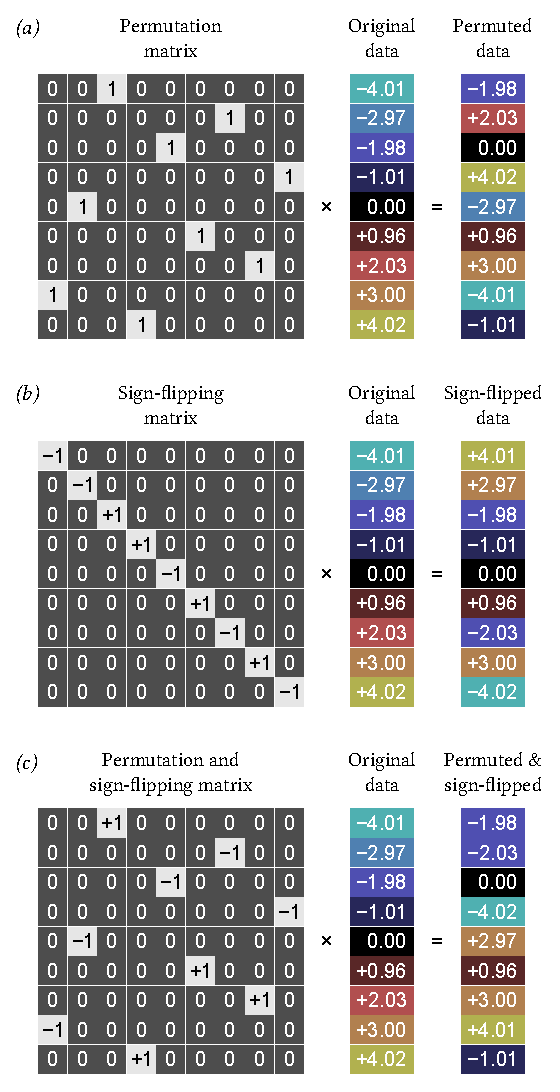
\includegraphics{images/pmatrices.eps}
\caption[Examples of permutation and sign flipping matrix.]{Examples of a permutation matrix (\emph{a}), of a sign flipping matrix (\emph{b}), and of a matrix that does permutation and sign flipping (\emph{c}). Pre-multiplication by a permutation matrix shuffles the order of the data, whereas by a sign flipping matrix changes the sign of a random subset of datapoints.}
\label{fig:perm:pmatrices}
\end{figure}

The essential assumption of permutation methods is that, for a given set of variables, \emph{their joint probability distribution does not change if the observations are rearranged}. This can be expressed in terms of exchangeable errors or independent and symmetric errors, each of these weakening different assumptions when compared to parametric methods.

\emph{Exchangeable errors} (\textsc{ee}) is the traditional permutation requirement \citep{Good2005}. The formal statement is that, for any permutation $\mathbf{P}_{j} \in \mathcal{P}$,

\begin{equation}
\boldsymbol{\epsilon} \stackrel{\mathrm{d}}{=} \mathbf{P}_{j}\boldsymbol{\epsilon}
\end{equation}

\noindent where the symbol $\stackrel{\mathrm{d}}{=}$ denotes equality of distributions. In other words, the errors are considered exchangeable if their joint distribution is invariant with respect to permutation. Exchangeability is similar to, yet more general than, independence, as exchangeable errors can have all-equal and homogeneous dependence. Relative to the common parametric assumptions of independent, normally and identically distributed (iid) errors, \textsc{ee} relaxes two aspects. First, normality is no longer assumed, although identical distributions are required. Second, the independence assumption is weakened slightly to allow exchangeability when the observations are not independent, but their joint distribution is maintained after permutation. While exchangeability is a general condition that applies to any distribution, the multivariate normal distribution is indeed exchangeable if the marginal distributions are uncorrelated, or if the off-diagonal elements of the covariance matrix are identical to each other (not necessarily equal to zero).\footnote{In parametric settings, such dependence structure is often referred to as \emph{compound symmetry}.}

\emph{Independent and symmetric errors} (\textsc{ise}) can be considered for measurements that arise, for instance, from differences between two groups if the variances are not assumed to be the same. The formal statement for permutation under \textsc{ise} is that for any sign flipping matrix $\mathbf{S}_{j} \in \mathcal{S}$,

\begin{equation}
\boldsymbol{\epsilon} \stackrel{\mathrm{d}}{=} \mathbf{S}_{j}\boldsymbol{\epsilon}
\end{equation}

\noindent
that is, the joint distribution of the error terms is invariant with respect to sign flipping. Relative to the parametric assumptions of independent, normally and identically distributed errors, \textsc{ise} relaxes normality, although symmetry of distributions is required. Independence is also required to allow sign flipping of one observation without perturbing others.

Although the \textsc{ee} does not require symmetry for the distribution of the error terms, it requires that the variances and covariances of the error terms are all equal, or have a structure that is compatible with the definition of exchangebility blocks (discussed below). While the \textsc{ise} assumption has yet more stringent requirements, if both \textsc{ee} and \textsc{ise} are plausible and available for a given model, permutations and sign flippings can be performed together, increasing the number of possible rearrangements, a feature particularly useful for studies with small sample sizes. The formal statement for shuffling under both \textsc{ee} and \textsc{ise} is that, as with the previous cases, for any matrix $\mathbf{B}_{j} \in \mathcal{B}$,

\begin{equation}
\boldsymbol{\epsilon} \stackrel{\mathrm{d}}{=} \mathbf{B}_{j}\boldsymbol{\epsilon}
\end{equation}

\noindent
that is, the joint distribution of the error terms remains unchanged under both permutation and sign flipping.

There are yet other important aspects related to exchangeability. The experimental design may dictate blocks of observations that are jointly exchangeable, allowing data to be permuted within block or, alternatively, that the blocks may themselves be exchangeable as a whole. This is the case, for instance, for designs that involve multiple observations from each subject. While permutation methods generally do not easily deal with non-independent data, the definition of these \emph{exchangeability blocks} (\textsc{eb}) allows these special cases of well structured dependence to be accommodated. While \textsc{eb} determine how the data shufflings are performed, they should not be confused with \emph{variance groups} (\textsc{vg}), i.e., groups of observations that are known or assumed to have similar variances, which can be pooled for estimation and computation of the statistic. Variance groups need to be compatible with, yet not necessarily identical to, the exchangeability blocks, as discussed in Section~\ref{sec:perm:restricted}. A summary of the properties discussed this far and some benefits of permutation methods are shown in Table~\ref{tab:perm:assumptions}.

\begin{table}[!p]
\caption[Summary of assumptions of permutation methods.]{Compared with parametric methods, permutation tests relax a number of assumptions and can be used in a wider variety of situations. Some of these assumptions can be further relaxed with the definition of exchangeability blocks.}
\begin{center}
{\small
\begin{tabular}{@{}l@{}m{17mm}<{\centering}m{13mm}<{\centering}m{17mm}<{\centering}@{}}
\toprule
Assumptions                                & \textsc{ee} & \textsc{ise} & Parametric\\
\midrule
\multicolumn{4}{l}{\emph{With respect to the dependence structure between error terms:}}\\
Independent                                & {\color{blue}\ding{'63}}  & {\color{blue}\ding{'63}}  & {\color{blue}\ding{'63}}\\
Non-independent, exchangeable              & {\color{blue}\ding{'63}}  & {\color{red}\ding{'67}}   & {\color{red}\ding{'67}}\\
Non-independent, non-exchangeable          & {\color{red}\ding{'67}}   & {\color{red}\ding{'67}}   & {\color{red}\ding{'67}}\\
\midrule
\multicolumn{4}{l}{\emph{With respect to the distributions of the error terms:}}\\
Normal, identical                          & {\color{blue}\ding{'63}}  & {\color{blue}\ding{'63}}  & {\color{blue}\ding{'63}}\\
Symmetrical, identical                     & {\color{blue}\ding{'63}}  & {\color{blue}\ding{'63}}  & {\color{red}\ding{'67}}\\
Symmetrical, non-identical                 & {\color{red}\ding{'67}}   & {\color{blue}\ding{'63}}  & {\color{red}\ding{'67}}\\
Skewed, identical                          & {\color{blue}\ding{'63}}  & {\color{red}\ding{'67}}   & {\color{red}\ding{'67}}\\
Skewed, non-identical                      & {\color{red}\ding{'67}}   & {\color{red}\ding{'67}}   & {\color{red}\ding{'67}}\\
\bottomrule
\end{tabular}}
{\footnotesize
\begin{enumerate}
\item[{\color{blue}\ding{'63}}] Can be used directly if the assumptions regarding dependence structure and \newline distribution of the error terms are both met.
\item[{\color{red}\ding{'67}}] Cannot be used directly, or can be used in particular cases.
\end{enumerate}\par}
\end{center}
\label{tab:perm:assumptions}
\end{table}

\subsubsection{Unrestricted exchangeability}
\label{sec:perm:unrestricted}

In the absence of nuisance variables, the model reduces to $\mathbf{Y}=\mathbf{X}\boldsymbol{\beta}+\boldsymbol{\epsilon}$, and under the null hypothesis $\mathcal{H}_0:\boldsymbol{\beta}=\boldsymbol{0}$ the data are pure error, $\mathbf{Y}=\boldsymbol{\epsilon}$.  Thus the \textsc{ee} or \textsc{ise} assumptions on the \emph{error} (presented above) justify freely permuting or sign flipping the \emph{data} under $\mathcal{H}_0$.  It is equivalent, however, to alter the design instead of the data. For example, for a nuisance-free design,

\begin{equation}
\mathbf{P}\mathbf{Y}=\mathbf{X}\boldsymbol{\beta}+\boldsymbol{\epsilon}\;\;\Longleftrightarrow\;\;
\mathbf{Y}=\mathbf{P}'\mathbf{X}\boldsymbol{\beta}+\mathbf{P}'\boldsymbol{\epsilon}
\end{equation}

\noindent
since permutation matrices $\mathbf{P}$ are orthogonal; the same holds for sign flipping matrices $\mathbf{S}$. This is an important computational consideration as altering the design is much less burdensome than altering the image data. Also note that the errors $\boldsymbol{\epsilon}$ are not observed and thus never directly altered; going forward we will suppress any notation indicating permutation or sign flipping of the errors.

In the presence of nuisance variables (Equation~\ref{eqn:perm:glmpart}), however, the problem is more complex. If the nuisance coefficients $\boldsymbol{\gamma}$ were somehow known, an exact permutation test would be available:

\begin{equation}
\mathbf{Y} - \mathbf{Z}\boldsymbol{\gamma} = \mathbf{P}\mathbf{X}\boldsymbol{\beta} + \boldsymbol{\epsilon}.
\end{equation}

The perfectly adjusted data $\mathbf{Y} - \mathbf{Z}\boldsymbol{\gamma}$ are then pure error under $\mathcal{H}_0$ and inference could proceed as above. In practice, the nuisance cofficients have to be estimated and the adjusted data will not behave as $\boldsymbol{\epsilon}$.  For example, the obvious solution is to use the nuisance-only residuals $\boldsymbol{\hat{\epsilon}}_{\mathbf{Z}}$ as the adjusted data.  However, as noted above, residuals induce dependence and any \textsc{ee} or \textsc{ise} assumptions on $\boldsymbol{\epsilon}$ will not be conveyed to $\boldsymbol{\hat{\epsilon}}_{\mathbf{Z}}$.

A number of approaches have been proposed to produce approximate p-values in these cases \citep{Draper1966, Beaton1978, Still1981, Brown1982, Levin1983, Freedman1983, Oja1987, Gail1988, Welch1990, TerBraak1992, Kennedy1995, Edgington1995, Huh2001, Jung2006, Manly2007, Kherad2010}. We present these methods in a common notation with detailed annotation in in Table~\ref{tab:perm:methods}.  While a number of authors have made comparisons between some of these methods \citep{Kennedy1995, Kennedy1996, Gonzalez1998, Anderson1999, Anderson2001, Anderson2003, OGorman2005, Dekker2007, Nichols2008, Ridgway2009}, they often only approached particular cases, did not consider repeated measurements, did not use full matrix notation as more common in neuroimaging literature, and often did not consider implementation complexities due to the large size of imaging datasets. In this section we focus on the Freedman--Lane and the Smith methods, which, as we show in Section~\ref{sec:perm:method_perm}, produce the best results in terms of control over error rates and power.

\begin{table}[p]
\caption[Methods available to construct the null distribution in the presence of nuisance variables.]{A number of methods are available to obtain parameter estimates and construct a reference distribution in the presence of nuisance variables.}
\begin{center}
{\small
\begin{tabular}{@{}m{3.9cm}r@{\hspace{1.8mm}}c@{\hspace{2.2mm}}l}
\toprule
Method &
\multicolumn{3}{c}{Model\hspace*{18mm}}\\
\midrule
%Exact$^{(a)}$ &
%$\mathbf{Y} - \mathbf{Z}\boldsymbol{\gamma}$ &$=$& $\mathbf{P}\mathbf{X}\boldsymbol{\beta} + \boldsymbol{\epsilon}$ \\
Draper--Stoneman$^{(a)}$ & 
$\mathbf{Y}$ &$=$& $\mathbf{P}\mathbf{X}\boldsymbol{\beta} + \mathbf{Z}\boldsymbol{\gamma} + \boldsymbol{\epsilon}$ \\
Still--White$^{(b)}$ &
$\mathbf{P}\mathbf{R}_{\mathbf{Z}}\mathbf{Y}$ &$=$& $\mathbf{X}\boldsymbol{\beta} + \boldsymbol{\epsilon}$  \\
Freedman--Lane$^{(c)}$ &
$\left(\mathbf{P}\mathbf{R}_{\mathbf{Z}}+\mathbf{H}_{\mathbf{Z}}\right)\mathbf{Y}$ &$=$& $\mathbf{X}\boldsymbol{\beta} + \mathbf{Z}\boldsymbol{\gamma}+\boldsymbol{\epsilon}$ \\
ter Braak$^{(d)}$ &
$\left(\mathbf{P}\mathbf{R}_{\mathbf{M}}+\mathbf{H}_{\mathbf{M}}\right)\mathbf{Y}$ &$=$& $\mathbf{X}\boldsymbol{\beta} + \mathbf{Z}\boldsymbol{\gamma}+\boldsymbol{\epsilon}$ \\
Kennedy$^{(e)}$ &
$\mathbf{P}\mathbf{R}_{\mathbf{Z}}\mathbf{Y}$ &$=$& $\mathbf{R}_{\mathbf{Z}}\mathbf{X}\boldsymbol{\beta} +  \boldsymbol{\epsilon}$ \\
Manly$^{(f)}$ &
$\mathbf{P}\mathbf{Y}$ &$=$& $\mathbf{X}\boldsymbol{\beta} + \mathbf{Z}\boldsymbol{\gamma} + \boldsymbol{\epsilon}$\\
Huh--Jhun$^{(g)}$ &
$\mathbf{P}\mathbf{Q}'\mathbf{R}_{\mathbf{Z}}\mathbf{Y}$ &$=$& $\mathbf{Q}'\mathbf{R}_{\mathbf{Z}}\mathbf{X}\boldsymbol{\beta} +  \boldsymbol{\epsilon}$\\
Smith$^{(h)}$ &
$\mathbf{Y}$ &$=$& $\mathbf{P}\mathbf{R}_{\mathbf{Z}}\mathbf{X}\boldsymbol{\beta} + \mathbf{Z}\boldsymbol{\gamma} + \boldsymbol{\epsilon}$ \\
Parametric$^{(i)}$ &
$\mathbf{Y}$ &$=$& $\mathbf{X}\boldsymbol{\beta} + \mathbf{Z}\boldsymbol{\gamma} + \boldsymbol{\epsilon},\;\; \boldsymbol{\epsilon}\sim\mathcal{N}(0,\sigma^2\mathbf{I})$ \\
\bottomrule
\end{tabular}}
\end{center}
{\footnotesize
%$(a)$ In the Exact method, the true $\boldsymbol{\gamma}$ is known and does not need to be estimated. Since it is known, $\mathbf{Z}\boldsymbol{\gamma}$ can be subtracted from $\mathbf{Y}$, and only $\boldsymbol{\beta}$ needs to be estimated. Permutation can be performed as for simple regression. The Exact method is used for comparison with the others in the simulations presented in Section~\ref{sec:perm:method_perm}.
$(a)$ \citet{Draper1966}. This method was called ``Shuffle~Z'' by \citet{Kennedy1995}, and using the same notation adopted here, it would be called ``Shuffle~X''.
$(b)$ \citet{Still1981, Levin1983, Gail1988}.
$(c)$ \citet{Freedman1983}.
$(d)$ \citet{TerBraak1992}. The null distribution for this method considers $\boldsymbol{\hat{\beta}}^{*}_{j} = \boldsymbol{\hat{\beta}}$, i.e., the permutation happens under the alternative hypothesis, rather than the null.
$(e)$ \citet{Kennedy1995, Kennedy1996}. This method was referred to as ``Residualize both Y and Z'' in the original publication, and using the same notation adopted here, it would be called ``Residualize both Y and X''.
$(f)$ \citet{Manly2007}.
$(g)$ \citet{Huh2001, Jung2006, Kherad2010}. $\mathbf{Q}$ is a $N \times N'$ matrix, where $N'$ is the rank of $\mathbf{R}_{\mathbf{Z}}$. $\mathbf{Q}$ is computed through Schur decomposition of $\mathbf{R}_{\mathbf{Z}}$, such that $\mathbf{R}_{\mathbf{Z}}=\mathbf{Q}\mathbf{Q}'$ and $\mathbf{I}_{N' \times N'}=\mathbf{Q}'\mathbf{Q}$. For this method, $\mathbf{P}$ is $N' \times N'$. From the methods in the table, this is the only that cannot be used directly under restricted exchangeability, as the block structure is not preserved.
$(h)$ The Smith method consists of orthogonalization of $\mathbf{X}$ with respect to $\mathbf{Z}$. In the permutation and multiple regression literature, this method was suggested by a referee of \citet{OGorman2005}, and later presented by \citet{Nichols2008} and discussed by \citet{Ridgway2009}.
$(i)$ The parametric method does not use permutations, being instead based on distributional assumptions.\
$\square$ For all the methods, the left side of the equations contains the data (regressand), the right side the regressors and error terms. The unpermuted models can be obtained by replacing $\mathbf{P}$ for $\mathbf{I}$. Even for the unpermuted models, and even if $\mathbf{X}$ and $\mathbf{Z}$ are orthogonal, not all these methods produce the same error terms $\boldsymbol{\epsilon}$. This is the case, for instance, of the Kennedy and Huh--Jhun methods. Under orthogonality between $\mathbf{X}$ and $\mathbf{Z}$, some regression methods are equivalent to each other.}
\label{tab:perm:methods}
\end{table}

The \emph{Freedman--Lane procedure} \citep{Freedman1983} can be performed through the following steps:

\begin{enumerate}
\item Regress $\mathbf{Y}$ against the full model that contains both the effects of interest and the nuisance variables, i.e.\ $\mathbf{Y} = \mathbf{X}\boldsymbol{\beta} + \mathbf{Z}\boldsymbol{\gamma} + \boldsymbol{\epsilon}$. Use the estimated parameters $\boldsymbol{\hat{\beta}}$ to compute the statistic of interest, and call this statistic $T_{0}$.
\item Regress $\mathbf{Y}$ against a reduced model that contains only the nuisance effects, i.e.\ $\mathbf{Y} = \mathbf{Z}\boldsymbol{\gamma} + \boldsymbol{\epsilon}_{\mathbf{Z}}$, obtaining estimated parameters $\boldsymbol{\hat{\gamma}}$ and estimated residuals $\boldsymbol{\hat{\epsilon}}_{\mathbf{Z}}$.
\item Compute a set of permuted data $\mathbf{Y}^{*}_{j}$. This is done by pre-multiplying the residuals from the reduced model produced in the previous step, $\boldsymbol{\hat{\epsilon}}_{\mathbf{Z}}$, by a permutation matrix, $\mathbf{P}_{j}$, then adding back the estimated nuisance effects, i.e.\ $\mathbf{Y}^{*}_{j} = \mathbf{P}_{j}\boldsymbol{\hat{\epsilon}}_{\mathbf{Z}} + \mathbf{Z}\boldsymbol{\hat{\gamma}}$. 
\item Regress the permuted data $\mathbf{Y}^{*}_{j}$ against the full model, i.e.\ $\mathbf{Y}^{*}_{j} = \mathbf{X}\boldsymbol{\beta} + \mathbf{Z}\boldsymbol{\gamma} + \boldsymbol{\epsilon}$, and use the estimated $\boldsymbol{\hat{\beta}}^{*}_{j}$ to compute the statistic of interest. Call this statistic $T^{*}_{j}$.
\item Repeat the Steps 2--4 many times to build the reference distribution of $T^{*}$ under the null hypothesis.
\item Count how many times $T^{*}_{j}$ was found to be equal or larger than $T_{0}$, and divide the count by the number of permutations; the result is the p-value.
\end{enumerate}

For the Steps 2 and 3, it is not necessary to actually fit the reduced model at each point in the image. The permuted dataset can equivalently be obtained as $\mathbf{Y}^{*}_{j} = \left(\mathbf{P}_{j}\mathbf{R}_{\mathbf{Z}}+\mathbf{H}_{\mathbf{Z}}\right)\mathbf{Y}$, which is particularly efficient for neuroimaging applications in the typical case of a single design matrix for all image points, as the term $\mathbf{P}_{j}\mathbf{R}_{\mathbf{Z}}+\mathbf{H}_{\mathbf{Z}}$ is then constant throughout the image and so, needs to be computed just once. Moreover, add the nuisance variables back in Step 3 is not strictly necessary, and the model can be expressed simply as $\mathbf{P}_{j}\mathbf{R}_{\mathbf{Z}}\mathbf{Y}=\mathbf{X}\boldsymbol{\beta}+\mathbf{Z}\boldsymbol{\gamma}+\boldsymbol{\epsilon}$, implying that the permutations can actually be performed just by permuting the rows of the residual-forming matrix $\mathbf{R}_{\mathbf{Z}}$. The Freedman--Lane strategy is the one used in the randomise algorithm, discussed in \ref{sec:perm:randomise}.

The rationale for this permutation method is that, if the null hypothesis is true, then $\boldsymbol{\beta}=\mathbf{0}$, and so the residuals from the reduced model with only nuisance variables, $\boldsymbol{\epsilon}_{\mathbf{Z}}$, should not be different than the residuals from the full model, $\boldsymbol{\epsilon}$, and can, therefore, be used to create the reference distribution from which p-values can be obtained.

The \emph{Smith procedure} consists of orthogonalising the regressors of interest with respect to the nuisance variables. This is done by pre-multiplication of $\mathbf{X}$ by the residual forming matrix due to $\mathbf{Z}$, i.e., $\mathbf{R}_{\mathbf{Z}}$, then permuting this orthogonalised version of the regressors of interest. The nuisance regressors remain in the model.\footnote{We name this method after Smith because, although orthogonalisation is a well known procedure, it does not seem to have been proposed by anyone to address the issues with permutation methods with the \textsc{glm} until Smith and others presented it in a conference poster \citep{Nichols2008}. We also use the eponym to keep it consistent with \citet{Ridgway2009}, and to keep the convention of calling the methods by the earliest author that we could identify as the proponent for each method, even though this method seems to have been proposed by an anonymous referee of \citet{OGorman2005}.}

For both the Freedman--Lane and the Smith procedures, if the errors are independent and symmetric (\textsc{ise}), the permutation matrices $\mathbf{P}_{j}$ can be replaced for sign flipping matrices $\mathbf{S}_{j}$. If both \textsc{ee} and \textsc{ise} are considered appropriate, then permutation and sign flipping can be used concomitantly.

\subsubsection{Restricted exchangeability}
\label{sec:perm:restricted}

Some experimental designs involve multiple observations from each subject, or the subjects may come from groups that may possess characteristics that may render their distributions not perfectly comparable. Both situations violate exchangeability. However, when the dependence between observations has a block structure, this structure can be taken into account when permuting the model, restricting the set of all otherwise possible permutations to only those that respect the relationship between observations \citep{Pesarin2001}.\footnote{Observations that are exchangeable only in some subsets of all possible permutations are said \emph{weakly exchangeable} \citep{Good2002}.} The \textsc{ee} and \textsc{ise} assumptions are then asserted at the level of these exchangeability blocks, rather than for each observation individually. The experimental hypothesis and the study design determine how the \textsc{eb}s should be formed and how the permutation or sign flipping matrices should be constructed. Except Huh--Jhun, the other methods can be applied at the block level as in the unrestricted case.

\paragraph{Within-block exchangeability}

Observations that share the same dependence structure, either assumed or known in advance, can be used to define \textsc{eb}s such that \textsc{ee} are asserted with respect to these blocks only, and the empirical distribution is constructed by permuting exclusively within block, as shown in Figure~\ref{fig:perm:within-block}. Once the blocks have been defined, the regression of nuisance variables and the construction of the reference distribution can follow strategies as Freedman--Lane or Smith, as above. The \textsc{ise}, when applicable, is transparent to this kind of block structure, so that the sign flips occur as under unrestricted exchangeability. For within-block exchangeability, in general each \textsc{eb} corresponds to a \textsc{vg} for the computation of the test statistic. See \ref{sec:perm:examples} for examples.

\begin{figure}[!p]
\centering
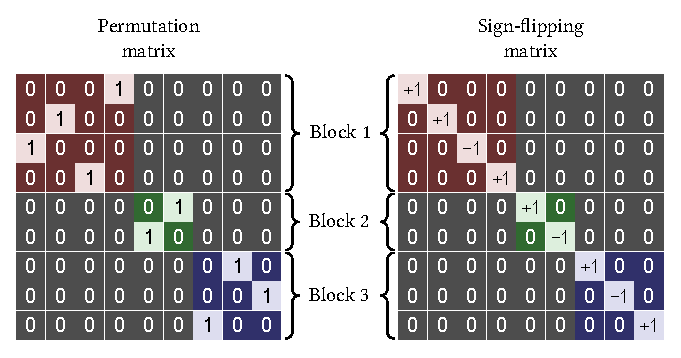
\includegraphics{images/within-block.eps}
\caption[Example of permutation and sign flipping matrix for within-block exchangeability]{\emph{\emph{Left:}} Example of a permutation matrix that shuffles data within block only. The blocks are not required to be of the same size. The elements outside the diagonal blocks are always equal to zero, such that data cannot be swapped across blocks. \emph{Right:} Example of a sign flipping matrix. Differently than within-block permutation matrices, here sign flipping matrices are transparent to the definitions of the blocks, such that the block definitions do not need to be taken into account, albeit their corresponding variance groups are considered when computing the statistic.}
\label{fig:perm:within-block}
\end{figure}

\paragraph{Whole-block exchangeability}

Certain experimental hypotheses may require the comparison of sets of observations to be treated as a whole, being not exchangeable within set. Exchangeability blocks can be constructed such that each include, in a consistent order, all the observations pertaining to a given set and, differently than in within-block exchangeability, here each block is exchanged with the others on their entirety, while maintaining the order of observations within block unaltered. For \textsc{ise}, the signs are flipped for all observations within block at once. Variance groups are not constructed one per block; instead, each \textsc{vg} encompasses one or more observations per block, all in the same order, e.g., one \textsc{vg} with the first observation of each block, another with the second of each block and so on. Consequently, all blocks must be of the same size, and all with their observations ordered consistently, either for \textsc{ee} or for \textsc{ise}. Examples of permutation and sign flipping matrices for whole block permutation are shown in Figure~\ref{fig:perm:whole-block}. See \ref{sec:perm:examples} for examples.

\begin{figure}[!p]
\centering
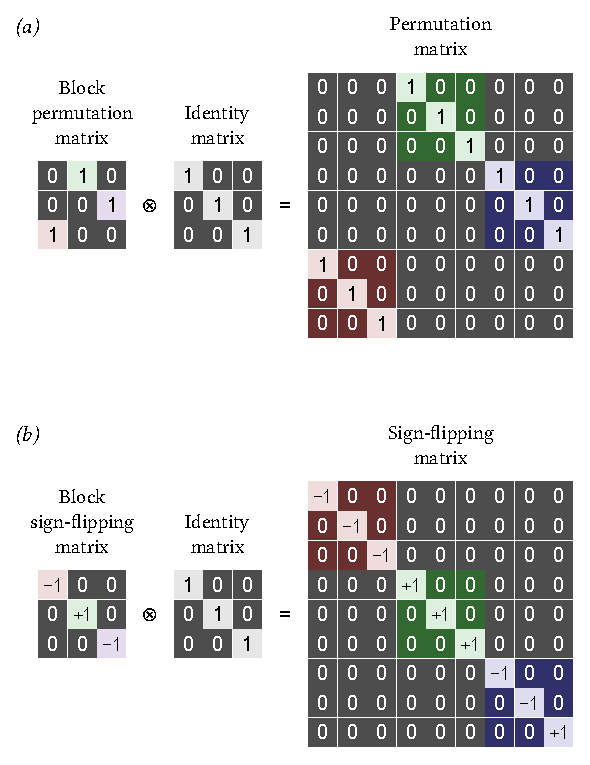
\includegraphics{images/whole-block.eps}
\caption[Example of permutation and sign flipping matrix for whole-block exchangeability]{(\emph{a}) Example of a permutation matrix that shuffles whole blocks of data. The blocks need to be of the same size. (\emph{b}) Example of a sign flipping matrix that changes the signs of the blocks as a whole. Both matrices can be constructed by the Kronecker product (represented by the symbol $\otimes$) of a permutation or a sign flipping matrix (with size determined by the number of blocks) and an identity matrix (with size determined by the number of observations per block).}
\label{fig:perm:whole-block}
\end{figure}

\paragraph{Variance groups mismatching exchangeability blocks} While variance groups can be defined implicity, as above, according to whether within- or whole-block permutation is to be perfomed, this is not compulsory. In some cases the \textsc{eb}s are defined based on the non-independence between observations, even if the variances across all observations can still be assumed to be identical. See \ref{sec:perm:examples} for an example using a paired $t$-test.

\paragraph{Choice of the statistic with exchangebility blocks} The statistics $F$ and $t$, described in Section~\ref{sec:perm:model}, are pivotal and follow known distributions when, among other assumptions, the error terms for all observations are identically distributed. Under these assumptions, all the errors terms can be pooled to compute the residual sum of squares (the term $\boldsymbol{\hat{\epsilon}}'\boldsymbol{\hat{\epsilon}}$ in the Equation~\ref{eqn:perm:fstat}) and so, the variance of the parameter estimates. This forms the basis for parametric inference, and is also useful for non-parametric tests. However, the presence of \textsc{eb}s is incompatible with the equality of distributions across all observations, with the undesired consequence that pivotality is lost, as shown in Sections~\ref{sec:perm:method_statistic} and \ref{sec:perm:results_statistic}. Although these statistics can still be used with permutation methods in general, the lack of pivotality for imaging applications can cause problems for correction for multiple testing. When exchangebility blocks are present, a suitable statistic can be computed as:

\begin{equation}
G = \dfrac{\boldsymbol{\hat{\psi}}'\mathbf{C} \left(\mathbf{C}'(\mathbf{M}'\mathbf{W}\mathbf{M})^{-1}\mathbf{C} \right)^{-1} \mathbf{C}'\boldsymbol{\hat{\psi}}}{\Lambda \cdot \mathrm{rank}\left(\mathbf{C}\right)}
\label{eqn:perm:gstat}
\end{equation}

\noindent
where $\mathbf{W}$ is a $N \times N$ diagonal weighting matrix that has elements

\begin{equation}
W_{nn} = \dfrac{\sum_{n' \in g_{n}}R_{n'n'}}{\boldsymbol{\hat{\epsilon}}_{g_{n}}'\boldsymbol{\hat{\epsilon}}_{g_{n}}}
\end{equation}

\noindent where $g_{n}$ represents the variance group to which the $n$-th observation belongs, $R_{n'n'}$ is the $n'$-th diagonal element of the residual forming matrix, and $\boldsymbol{\hat{\epsilon}}_{g_{n}}$ is the vector of residuals associated with the same \textsc{vg}.\footnote{Note that, for clarity, $G$ is defined in Equation~\ref{eqn:perm:gstat} as a function of $\mathbf{M}$, $\boldsymbol{\psi}$ and $\mathbf{C}$ in the unpartitioned model. With the partitioning described in the \ref{sec:perm:partitioning}, each of these variables is replaced by their equivalents in the partitioned, full model, i.e., $[\mathbf{X} \; \mathbf{Z}]$, $[\boldsymbol{\beta}' \; \boldsymbol{\gamma}']'$ and $[\mathbf{I}_{s \times s}\;\mathbf{0}_{s \times (r-s)}]'$ respectively.} In other words, each diagonal element of $\mathbf{W}$ is the reciprocal of the estimated variance for their corresponding group. This variance estimator is equivalent to the one proposed by \citet{Horn1975}. The remaining term in Equation~\ref{eqn:perm:gstat} is given by \citep{Welch1951}:

\begin{equation}
\Lambda = 1+\frac{2(s-1)}{s(s+2)}\sum_{g} \frac{1}{\sum_{n \in g}R_{nn}} \left(1-\frac{\sum_{n \in g}W_{nn}}{\mathrm{trace}\left(\mathbf{W}\right)}\right)^2
\end{equation}

\noindent
where $s=\mathrm{rank}\left(\mathbf{C}\right)$ as before. The statistic $G$ provides a generalisation of a number of well known statistical tests, some of them summarised in Table~\ref{tab:perm:G}. When there is only one \textsc{vg}, variance estimates can be pooled across all observations, resulting in $\Lambda=1$ and so, $G=F$. If $\mathbf{W}=\mathbf{V}^{-1}$, the inverse of the true covariance matrix, $G$ is the statistic for an $F$-test in a weighted least squares model (\textsc{wls}) \citep{Christensen2002}. If there are multiple variance groups, $G$ is equivalent to the $v^2$ statistic for the problem of testing the means for these groups under no homoscedasticity assumption, i.e., when the variances cannot be assumed to be all equal \citep{Welch1951}.\footnote{If the errors are independent and normally distributed, yet not necessarily with equal variances (i.e., $\Lambda \neq 1$), parametric p-values for $G$ can be approximated by referring to the $F$-distribution with degrees of freedom $\nu_1=s$ and $\nu_2=2(s-1)/3(\Lambda-1)$.} If, despite heteroscedasticity, $\Lambda$ is replaced by 1, $G$ is equivalent to the James' statistic for the same problem \citep{James1951}. When $\mathrm{rank}\left(\mathbf{C}\right) = 1$, and if there are more than one \textsc{vg}, $\mathrm{sign}(\boldsymbol{\hat{\beta}})\sqrt{G}$ is the well-known $v$ statistic for the Behrens--Fisher problem \citep{Fisher1935_fid, Aspin1949}; with only one \textsc{vg} present, the same expression produces the Student's $t$ statistic, as shown earlier. If the definition of the blocks is respected, all these particular cases produce pivotal statistics, and the generalisation provided by $G$ allows straightforward implementation.

\begin{table}[!t]
\caption[Some tests of which the statistic $G$ is a generalisation.]{The statistic $G$ provides a generalisation for a number of well known statistical tests.}
\begin{center}
{\small
\begin{tabular}{@{}m{70mm}<{\raggedright}@{}m{25mm}<{\centering}m{25mm}<{\centering}@{}}
\toprule
{} & $\mathrm{rank}\left(\mathbf{C}\right) = 1$ & $\mathrm{rank}\left(\mathbf{C}\right) > 1$ \\
\midrule
Homoscedastic errors, unrestricted exchangeability ($\Lambda = 1$) & Square of Student's $t$ & $F$-ratio \\
\midrule
Homoscedastic within \textsc{vg}, restricted exchangeability ($\Lambda \neq 1$) & Square of Aspin--Welch $v$ & Welch's $v^2$\\
\bottomrule
\end{tabular}}
\end{center}
\label{tab:perm:G}
\end{table}

\subsection{Number of permutations} 

For a study with $N$ observations, the maximum number of possible permutations is $N!$, and the maximum number of possible sign flips is $2^N$. However, in the presence of $B$ exchangebility blocks that are exchangeable as a whole, the maximum number of possible permutations drops to no more than $B!$, and the maximum number of sign flips to $2^B$. For designs where data is only exchangeable within-block, the maximum number of possible permutations is $\prod_{b=1}^{B} N_{b}!$, where $N_{b}$ is the number of observations for the $b$-th block, and the maximum number of sign flips continues to be $2^N$.

However, the actual number of possible rearrangements may be smaller depending on the null hypothesis, the permutation strategy, or other aspects of the study design. If there are discrete covariates, or if there are ties among continuous regressors, many permutations may not alter the model at all. The maximum number of permutations can be calculated generically from the design matrix observing the number of repeated rows in $\mathbf{X}$ for the Freedman--Lane and most other methods, or in $\mathbf{M}$ for the ter Braak and Manly methods. The maximum number of possible permutations or sign flips, for different restrictions on exchangeability, is shown in Table~\ref{tab:perm:numperm}.

\begin{table}[p]
\caption[Maximum number of unique permutations.]{Maximum number of unique permutations considering exchangeability blocks.}
\begin{center}
{\small
\begin{tabular}{@{}m{62mm}<{\raggedright}m{44mm}<{\centering}@{}m{15mm}<{\centering}@{}}
\toprule
Exchangeability & \textsc{ee}   & \textsc{ise}\\
\midrule
Unrestricted & \[N!\] & \[2^N\]\\
\midrule
Unrestricted, repeated rows & \[N!\prod_{m=1}^M \frac{1}{N_m!}\] & \[2^N\] \\
\midrule
Within-block & \[\prod_{b=1}^{B} N_{b}!\] & \[2^N\] \\
\midrule
Within-block, repeated rows & \[\prod_{b=1}^{B} N_{b}! \prod_{m=1}^{M|b} \frac{1}{N_{m|b}!}\] & \[2^N\] \\
\midrule
Whole-block  & \[B!\] & \[2^B\]\\
\midrule
Whole-block, repeated blocks  & \[B!\prod_{\tilde{m}=1}^{\tilde{M}} \frac{1}{N_{\tilde{m}}!}\] & \[2^B\]\\
\bottomrule
\end{tabular}}
\end{center}
{\footnotesize
\begin{enumerate}
\item [$B$] Number of exchangebility blocks (\textsc{eb}).
\item [$M$] Number of distinct rows in $\mathbf{X}$.
\item [$M|b$] Number of distinct rows in $\mathbf{X}$ within the $b$-th block.
\item [$\tilde{M}$] Number of distinct blocks of rows in $\mathbf{X}$.
\item [$N$] Number of observations.
\item [$N_b$] Number of observations in the $b$-th block.
\item [$N_m$] Number of times each of the $M$ distinct rows occurs in $\mathbf{X}$.
\item [$N_{m|b}$] Number of times each of the $m$-th unique row occurs within the $b$-th block.
\item [$N_{\tilde{m}}$] Number of times each of the $\tilde{M}$ distinct blocks occurs in $\mathbf{X}$.
\end{enumerate}}
\label{tab:perm:numperm}
\end{table}

Even considering the restrictions dictacted by the study design, the number of possible shufflings tends to be very large, even for samples of moderate size, and grows very rapidly as observations are included. When the number of possible rearrangements is large, not all of them need to be performed for the test to be valid \citep{Dwass1957, Chung1958}, and the resulting procedure will be approximately exact \citep{Edgington1969}. The number can be chosen according to the availability of computational resources and considerations about power and precision. The smallest p-value that can be obtained is given by $1/J$, where $J$ is the number of permutations performed. The precision of permutation p-values may be determined considering the confidence interval around the significance level.

To efficiently avoid permutations that do not change the design matrix, the Algorithm ``\textsc{l}'' \citep{Knuth2005} can be used. This algorithm is simple and has the benefit of generating only permutations that are unique, i.e., in the presence of repeated elements, it correctly avoids synonymous permutations. This is appropriate when enumerating all possible permutations. However, the algorithm produces sequentially permutations that are in lexicographic order. Although this can be advantageous in other settings, here this behaviour can be problematic when running only a subset of $\mathcal{P}$, and has potential to bias the results. For imaging applications, where there are many points (voxels, vertices, faces) being analysed, it is in general computationally less expensive to shuffle many times a sequence of values and store these permuted sequences, than actually fit the permuted model for all points. As a consequence, the problem with lexicographically ordered permutations can be solved by generating all the possible permutations, and randomly drawing $J$ elements from $\mathcal{P}$ to do the actual shufflings of the model,  or generating random permutations and checking for duplicates. Alternatively, the procedure can be conducted without attention to repeated permutations using simple shuffling of the data. This strategy is known as \emph{conditional Monte Carlo} (\textsc{cmc}) \citep{Trotter1956, Pesarin2010}, as each of the random realisations is conditional on the available observed data.

Sign flipping matrices, on the other hand, can be listed using a numeral system with radix 2, and the sign flipped models can be performed without the need to enumerate all possible flips or to appeal to \textsc{cmc}. The simplest strategy is to use the digits $0$ and~$1$ of the binary numeral system, treating 0 as $-1$ when assembling the matrix. In a binary system, each sign flipping matrix is also its own numerical identifier, such that avoiding repeated sign flippings is trivial. The binary representation can be converted to and from radix 10 if needed, e.g., to allow easier human readability.

For within-block exchangeability, permutation matrices are constructed within-block, then concatenated along their diagonal to assemble $\mathbf{P}_{j}$, which also has a block structure. The elements outside the blocks are filled with zeros as needed  (Figure~\ref{fig:perm:within-block}). The block definitions can be ignored for sign flipping matrices for designs where \textsc{ise} is asserted within-block. For whole-block exchangeability, permutation and sign flipping matrices are generated by treating each block as an element, and the final $\mathbf{P}_{j}$ or $\mathbf{S}_{j}$ are assembled via Kronecker multiplication by an identity matrix of the same size as the blocks (Figure~\ref{fig:perm:whole-block}).

\subsection{Multiple testing}

Differently than with parametric methods, correction for multiple testing using permutation does not require the introduction of more assumptions. For familywise error rate correction (\textsc{fwer}), the method was described by \citet{Holmes1996}. As the statistics $T_{j}^{*}$ are calculated for each shuffling to build the reference distribution at each point, the maximum value of $T_{j}^{*}$ across the image, $T_{j}^{\text{max}}$, is also recorded for each rearrangement, and its empirical distribution is obtained. For each test in the image, an \textsc{fwer}-corrected p-value can then be obtained by computing the proportion of $T_{j}^{\text{max}}$ that is above $T_{0}$ for each test. A single \textsc{fwer} threshold can also be applied to the statistical map of $T_{0}$ values using the distribution of $T_{j}^{\text{max}}$. The same strategy can be used for statistics that combine spatial extent of signals, such as cluster extent or mass \citep{Bullmore1999}, threshold-free cluster enhancement (\textsc{tfce}) \citep{Smith2009} and others \citep{Marroquin2011}. For these spatial statistics, the effect of lack of pivotality can be mitigated by non-stationarity correction \citep{Hayasaka2004_nonstationary, Salimi-Khorshidi2011}.

The p-values under the null hypothesis are uniformly distributed in the interval $[0,1]$. As a consequence, the p-values themselves are
pivotal quantities and, in principle, could be used for multiple testing correction as above. The distribution of minimum p-value, $p_{j}^{\text{min}}$, instead of $T_{j}^{\text{max}}$, can be used. Due to the discreteness of the p-values, this approach, however, entails some computational difficulties that may cause considerable loss of power \citep{Pantazis2005}. Correction based on false-discovery rate (\textsc{fdr}) can be used once the uncorrected p-values have been obtained for each point in the image. Either a single \textsc{fdr} threshold can be applied to the map of uncorrected p-values \citep{Benjamini1995, Genovese2002} or an \textsc{fdr}-adjusted p-value can be calculated at each point \citep{Yekutieli1999}.

\subsection{The randomise algorithm}
\label{sec:perm:randomise}

Algorithm~1 describes a procedure for permutation inference on contrasts of the \textsc{glm} parameter estimates using the Freedman--Lane method. Modifications for other methods are trivial. For this algorithm, consider $\mathbf{Y}$ as a four-dimensional array, being the first three dimensions for space and the last for an observation index. A variable $\mathbf{v}=[x, y, z]$ is used to specify the point position in space, so that the vector of $n$ different observations per point is represented as $\mathbf{Y}[\mathbf{v}]$. A set $\mathcal{C}$ of contrasts is specified, as well as the unpartitioned design matrix $\mathbf{M}$. Indicator variables are used to specify whether the errors should be treated as exchangeable ($\textsc{ee}=\textsc{true}$), independent and symmetric ($\textsc{ise}=\textsc{true}$), or both, which allows for permutations to happen together with sign flipping. A positive integer $J$ is specified as the number permutations to be performed. Optionally, a $n \times 1$ vector $\mathbf{b}$ is provided to indicate the $B$ exchangebility blocks that group the observations, along with an indicator variable $\textsc{pb}$ that informs whether blocks should be permuted as a whole ($\textsc{pb} = \textsc{true}$), or if permutations should happen within block only ($\textsc{pb} = \textsc{false}$). The specification of $\mathbf{b}$ and \textsc{pb} obviate the need to specify the variance groups, as these can be defined implicitly for within or whole-block permutation when the pivotal statistic is computed.

\vspace{4mm}
\singlespacing
\noindent \textsf{Algorithm 1: The randomise algorithm.}\\
\HRule
\vspace{1mm}
{\small
\begin{algorithmic}[1]
\Require $\mathbf{Y}, \mathbf{M}, \mathcal{C}, \textsc{ee}, \textsc{ise}, J$. \textbf{Optional:} $\mathbf{b}, \textsc{pb}$.
\Comment{Input variables.}
\If{\textlnot\ \textsf{exist}(\textsc{pb})}
\Comment{If \textsc{pb} was not provided.}
\State $\textsc{pb} \leftarrow \textsc{false}$
\Comment{Permutations happen within block.}
\EndIf
\If{\textlnot\ \textsf{exist}($\mathbf{b}$)}
\Comment{If $\mathbf{b}$ was not provided.}
\State $\mathbf{b} \leftarrow \mathbf{1}_{n \times 1}$
\Comment{A vector of ones is used for $\mathbf{b}$.}
\State $\textsc{pb} \leftarrow \textsc{false}$
\Comment{Permutations happen within the single block.}
\EndIf
\ForAll{$\mathbf{C} \in \mathcal{C}$}
\Comment{For each contrast.}
\State $\mathbf{X}, \mathbf{Z} \leftarrow \text{\textsf{partition}}(\mathbf{M}, \mathbf{C})$
\Comment{Partition the model.}
\State $\mathbf{M} \leftarrow [\mathbf{X}\;\mathbf{Z}]$
\Comment{For simplicity, replace $\mathbf{M}$.}
\State $J^{\text{max}} \leftarrow \text{\textsf{calc\_maxshuf}}(\mathbf{X}, \mathbf{b}, \textsc{pb}, \textsc{ee}, \textsc{ise})$
\Comment{Maximum possible shufflings.}
\If {$\textsc{ee}$}
\Comment{If errors are exchangeable.}
\If {$J \geqslant J^{\text{max}}$}
\Comment{Exhaustive or too many permutations requested.}
\State $\mathcal{P} \leftarrow \text{\textsf{algorithm\_L}}(\mathbf{X}, \mathbf{b}, \textsc{pb})$
\Comment{List all possible permutations.}
\Else
\State $\mathcal{P} \leftarrow \text{\textsf{permute\_randomly}}(\mathbf{X}, \mathbf{b}, \textsc{pb}, J-1)$
\Comment{Ignore repeated $\mathbf{P}_{j}$.}
\State $\mathcal{P} \leftarrow \{\mathcal{P},\mathbf{I}\}$
\Comment{Ensure inclusion of the unpermuted model.}
\EndIf
\EndIf
\If {$\textsc{ise}$}
\Comment{If errors are independent and symmetric.}
\If {$J \geqslant J^{\text{max}}$}
\Comment{Exhaustive or too many sign flips requested.}
\State $\mathcal{S} \leftarrow \text{\textsf{list\_signflips}}(\mathbf{b}, \textsc{pb})$
\Comment{List all possible sign flippings.}
\Else
\State $\mathcal{S} \leftarrow \text{\textsf{signflip\_randomly}}(n, \mathbf{b}, \textsc{pb}, J-1)$
\Comment{Ignore repeated $\mathbf{S}_{j}$.}
\State $\mathcal{S} \leftarrow \{\mathcal{S},\mathbf{I}\}$
\Comment{Ensure inclusion of the non-sign flipped model.}
\EndIf
\EndIf
\If {$\textsc{ee}$ $\wedge$ $\textsc{ise}$}
\Comment{Errors independent, symmetric and exchangeable.}
\State $\mathcal{B} \leftarrow \text{\textsf{draw\_products}}(\mathcal{P}, \mathcal{S}, J)$
\Comment{Draw $J$ random products $\mathbf{P}_{j'}\mathbf{S}_{j''}$.}
\If {$\mathbf{I} \notin \mathcal{B}$}
\Comment{If non-shuffled model is absent from $\mathcal{B}$.}
\State $\mathcal{B} \leftarrow \{\mathbf{B}_{1},\ldots,\mathbf{B}_{J-1},\mathbf{I}\}$
\Comment{Ensure non-shuffled model is included.}
\EndIf
\State $\mathcal{B} \leftarrow \mathcal{P}$
\Comment{Treat $\mathcal{B}$ as $\mathcal{P}$ for simplicity.}
\ElsIf {$\textsc{ise}$ $\wedge$ \textlnot\ $\textsc{ee}$}
\Comment{If errors are only independent and symmetric.}
\State $\mathcal{P} \leftarrow \mathcal{S}$
\Comment{Treat $\mathcal{S}$ as $\mathcal{P}$ for simplicity.}
\EndIf
\ForAll{$\mathbf{v}$}
\Comment{For each image point.}
\State $\mathbf{U}[\mathbf{v}] \leftarrow 0$
\Comment{Initialise counter for uncorrected p-value.}
\State $\mathbf{F}[\mathbf{v}] \leftarrow 0$
\Comment{Initialise counter for \textsc{fwer}-corrected p-value.}
\State $\boldsymbol{\hat{\epsilon}}_{\mathbf{Z}}[\mathbf{v}] \leftarrow (\mathbf{I}-\mathbf{Z}\mathbf{Z}^{+})\mathbf{Y}[\mathbf{v}]$
\Comment{Remove the nuisance effects.}
\State $\boldsymbol{\hat{\psi}}[\mathbf{v}] \leftarrow \mathbf{M}^{+}\boldsymbol{\hat{\epsilon}}_{\mathbf{Z}}[\mathbf{v}]$
\Comment{Estimate regression coefficients.}
\State $\boldsymbol{\hat{\epsilon}}[\mathbf{v}] \leftarrow (\mathbf{I}-\mathbf{M}\mathbf{M}^{+})\boldsymbol{\hat{\epsilon}}_{\mathbf{Z}}[\mathbf{v}]$
\Comment{Estimate the residuals.}
\State $\mathbf{T}_{0}[\mathbf{v}] \leftarrow \text{\textsf{pivotal}}(\boldsymbol{\hat{\psi}}[\mathbf{v}],\boldsymbol{\hat{\epsilon}}[\mathbf{v}],\mathbf{M},\mathbf{b},\text{\textsc{pb}})$
\Comment{Compute a pivotal statistic.}
\EndFor
\For{$\mathbf{P}_{j} \in \mathcal{P}$}
\Comment{For each shuffling (permutation and/or sign flipping).}
\State $\mathbf{M}_{j}^{*} \leftarrow \mathbf{P}_{j}\mathbf{M}$
\Comment{Shuffle the model.}
\ForAll{$\mathbf{v}$}
\Comment{For each image point.}
\State $\boldsymbol{\hat{\psi}}_{j}^{*}[\mathbf{v}] \leftarrow (\mathbf{M}_{j}^{*})^{+}\boldsymbol{\hat{\epsilon}}_{\mathbf{Z}}[\mathbf{v}]$
\Comment{Fit permuted model.}
\State $\boldsymbol{\hat{\epsilon}}_{j}^{*}[\mathbf{v}] \leftarrow (\mathbf{I}-\mathbf{M}_{j}^{*}(\mathbf{M}_{j}^{*})^{+})\boldsymbol{\hat{\epsilon}}_{\mathbf{Z}}[\mathbf{v}]$
\Comment{Residuals.}
\State $\mathbf{T}_{j}^{*}[\mathbf{v}] \leftarrow \text{\textsf{pivotal}}(\boldsymbol{\hat{\psi}}_{j}^{*}[\mathbf{v}],\boldsymbol{\hat{\epsilon}}_{j}^{*}[\mathbf{v}],\mathbf{M}_{j}^{*},\mathbf{b},\text{\textsc{pb}})$
\Comment{Shuffled statistic.}
\If{$\mathbf{T}_{j}^{*}[\mathbf{v}] \geqslant \mathbf{T}_{0}[\mathbf{v}]$}
\Comment{If shuffled statistic is larger.}
\State $\mathbf{U}[\mathbf{v}] \leftarrow \mathbf{U}[\mathbf{v}]+1$
\Comment{Increment counter for uncorrected.}
\EndIf
\EndFor
\State $T^{\text{max}}_{j} \leftarrow \text{\textsf{max}}(\mathbf{T}_{j}^{*})$
\Comment{Find the largest $T_{j}^{*}$ across space.}
\ForAll{$\mathbf{v}$}
\Comment{For each image point.}
\If{$T^{\text{max}}_{j} \geqslant \mathbf{T}_{0}[\mathbf{v}]$}
\Comment{If $T_{j}^{\text{max}}$ is larger.}
\State $\mathbf{F}[\mathbf{v}] \leftarrow \mathbf{F}[\mathbf{v}]+1$
\Comment{Increment counter for \textsc{fwer}-corrected.}
\EndIf
\EndFor
\EndFor
\State p-value $\leftarrow \mathbf{U} / J$
\Comment{Significance map for this $\mathbf{C}$, uncorrected.}
\State p$_{\text{\textsc{fwer}}}$-value $\leftarrow \mathbf{F} / J$
\Comment{Significance map for this $\mathbf{C}$, \textsc{fwer}-corrected.}
\State \Return p-value, p$_{\text{\textsc{fwer}}}$-value.
\Comment{Save significance images to disk.}
\EndFor
\end{algorithmic}}
\noindent
\HRule\\
\setstretch{\lspac}
\vspace{0mm}

In the algorithm, the statistics $T$ for each point (voxel, vertex, face) are stored in the array $\mathbf{T}$, whereas the counters are stored in the arrays $\mathbf{U}$ and $\mathbf{F}$. The design matrix as well as the contrasts can be specific for each image point (voxelwise, vertexwise, facewise), and there is no challenge other than implementation. It is possible to omit the for-loop between lines 56 and 60, and instead store the distribution of the largest statistic as a vector of size $J$, which is then used to assess significance. The code runs faster, but it would be slightly less clear to present. In programming languages that offer good matrix manipulation capabilities, e.g.\ Octave, \textsc{matlab} or \textsc{r}, the for-loops that iterate for each point $\mathbf{v}$ can be replaced by matrix operations that are executed all in a single step. In the \textsc{Fmrib} Software Library (\textsc{fsl})\footnote{Available for download at \href{http://www.fmrib.ox.ac.uk/fsl}{\texttt{http://www.fmrib.ox.ac.uk/fsl}}.}, a fast implementation, in \textsc{c}++, of the randomise algorithm is available.

\section{Worked examples}
\label{sec:perm:examples}

The examples below serve to illustrate the permutation aspects discussed in the chapter, all with tiny samples, $N=12$ only, so that the design matrices can be shown in their full extent. While permutation tests in general remain valid even with such small samples, these examples are by no means to be understood as a recommendation for sample sizes. There are many reasons why larger samples are more appropriate (see \citet{Button2013} for a recent review), and in what concerns permutations methods, larger samples allow smaller p-values, improve the variance estimates for each \textsc{vg} (which are embodied in the weighting matrix under restricted exchangeability), and allow finer control over the familywise error rate. For each example, the relevant contrasts are also shown.

\paragraph{Example 1: Mean effect} Consider a multi-subject \textsc{fmri} study to investigate the \textsc{bold} response associated with a novel experimental task. After the first-level analysis (within subject), maps of contrasts of parameter estimates for each subject are used in a second level analysis. The design matrix for the mean effect is simply a column of ones, and permutations of the data or of the design matrix do not change the model with respect to the regressor of interest. However, by treating the errors as symmetric, instead of permutation, the signs of the ones in the design matrix, or of each datapoint, can be flipped randomly to create the empirical distribution from which inference can be performed. In the presence of nuisance variables, such as handedness, the procedure is performed as in either the Freedman--Lane or Smith methods, replacing the permutation matrix for a sign flipping matrix (Table~\ref{tab:perm:ex_meaneffect}).

\begin{table}[!t]
\caption[Coding for Example 1]{Coding of the design matrix, exchangeability blocks and variance groups for \textbf{Example~1}. Under unrestricted exchangeability, all subjects are assigned to a single block, and with identical variances, all to a single variance group. The regressor $\mathbf{m}_1$ codes for the overall mean, whereas $\mathbf{m}_2$ codes for handedness.}
\begin{center}
{\small
\begin{tabular}{@{}lccrr@{}}
\toprule
\multirow{2}{*}{\vspace*{-1.7mm}Coded data ($\mathbf{Y}$)} & \multirow{2}{*}{\vspace*{-1.7mm}\textsc{eb}} & \multirow{2}{*}{\vspace*{-1.7mm}\textsc{vg}} & \multicolumn{2}{c}{Model ($\mathbf{M}$)\hspace*{-2mm}}\\
\cmidrule(l){4-5}
& & &  $\mathbf{m}_1$ & $\mathbf{m}_2$\\
\midrule
Subject 1  & 1 & 1 & 1 & $h_{1}$\\
Subject 2  & 1 & 1 & 1 & $h_{2}$\\
Subject 3  & 1 & 1 & 1 & $h_{3}$\\
Subject 4  & 1 & 1 & 1 & $h_{4}$\\
Subject 5  & 1 & 1 & 1 & $h_{5}$\\
Subject 6  & 1 & 1 & 1 & $h_{6}$\\
Subject 7  & 1 & 1 & 1 & $h_{7}$\\
Subject 8  & 1 & 1 & 1 & $h_{8}$\\
Subject 9  & 1 & 1 & 1 & $h_{9}$\\
Subject 10 & 1 & 1 & 1 & $h_{10}$\\
Subject 11 & 1 & 1 & 1 & $h_{11}$\\
Subject 12 & 1 & 1 & 1 & $h_{12}$\\
\midrule
Contrast 1 ($\mathbf{C}'_1$) & & & $+1$ & 0\\
Contrast 2 ($\mathbf{C}'_2$) & & & $-1$ & 0\\
\bottomrule
\end{tabular}}
\end{center}
\label{tab:perm:ex_meaneffect}
\end{table}

\paragraph{Example 2: Multiple regression} Consider the analysis of a study that compares patients and controls with respect to brain cortical thickness, and that recruiting process ensured that all selected subjects are exchangeable. Elder subjects may, however, have thinner cortices, regardless of the diagnosis so, without considering the possibility of interaction. To control for the confounding effect of age, it is included in the design as a nuisance regressor. Sex is also included. The permutation strategy follows the Freedman--Lane or Smith methods, with the residuals of the reduced model being permuted under unrestricted exchangeability (Table~\ref{tab:perm:ex_multipleregression}).

\begin{table}[!t]
\caption[Coding for Example 2]{Coding for \textbf{Example~2}. Under unrestricted exchangeability, all subjects are assigned to a single block. The regressors $\mathbf{m}_1$ and $\mathbf{m}_2$ code for the experimental groups, $\mathbf{m}_3$ and $\mathbf{m}_4$ for age and sex.}
\begin{center}
{\small
\begin{tabular}{@{}lccrrrr@{}}
\toprule
\multirow{2}{*}{\vspace*{-1.7mm}Coded data ($\mathbf{Y}$)} & \multirow{2}{*}{\vspace*{-1.7mm}\textsc{eb}} & \multirow{2}{*}{\vspace*{-1.7mm}\textsc{vg}} & \multicolumn{4}{c}{Model ($\mathbf{M}$)\hspace*{-3mm}}\\
\cmidrule(l){4-7}
& & & $\mathbf{m}_1$ & $\mathbf{m}_2$ & $\mathbf{m}_3$ & $\mathbf{m}_4$\\
\midrule
Subject 1   & 1 & 1 & 1 & 0 & $a_{1}$  & $s_{1}$\\
Subject 2   & 1 & 1 & 1 & 0 & $a_{2}$  & $s_{2}$\\
Subject 3   & 1 & 1 & 1 & 0 & $a_{3}$  & $s_{3}$\\
Subject 4   & 1 & 1 & 1 & 0 & $a_{4}$  & $s_{4}$\\
Subject 5   & 1 & 1 & 1 & 0 & $a_{5}$  & $s_{5}$\\
Subject 6   & 1 & 1 & 1 & 0 & $a_{6}$  & $s_{6}$\\
Subject 7   & 1 & 1 & 0 & 1 & $a_{7}$  & $s_{7}$\\
Subject 8   & 1 & 1 & 0 & 1 & $a_{8}$  & $s_{8}$\\
Subject 9   & 1 & 1 & 0 & 1 & $a_{9}$  & $s_{9}$\\
Subject 10  & 1 & 1 & 0 & 1 & $a_{10}$ & $s_{10}$\\
Subject 11  & 1 & 1 & 0 & 1 & $a_{11}$ & $s_{11}$\\
Subject 12  & 1 & 1 & 0 & 1 & $a_{12}$ & $s_{12}$\\
\midrule
Contrast 1 ($\mathbf{C}'_1$) & & & $+1$ & $-1$ & 0 & 0\\
Contrast 2 ($\mathbf{C}'_2$) & & & $-1$ & $+1$ & 0 & 0\\
\bottomrule
\end{tabular}}
\end{center}
\label{tab:perm:ex_multipleregression}
\end{table}

\paragraph{Example 3: Paired $t$-test} Consider a study to investigate the effect of the use of a certain analgesic in the magnitude of the \textsc{bold} response associated with painful stimulation. In this example, the response after the treatment is compared with the response before the treatment, i.e., each subject is their own control. The experimental design is the ``paired $t$-test''. One \textsc{eb} is defined per subject, as the observatios are not exchangeable across subjects, and as the variance can be assumed to be homogeneous across all observations, only one \textsc{vg} is defined encompassing all observations (Table~\ref{tab:perm:ex_pairedttest}).

\begin{table}[!t]
\caption[Coding for Example 3]{Coding of the design matrix exchangebility blocks and variance groups for \textbf{Example~3}. Observations are exchangeable only within subject, and variance can be estimated considering all observations as a single group. The regressor $\mathbf{m}_1$ codes for treatment, whereas $\mathbf{m}_2$ to $\mathbf{m}_7$ code for subject-specific mean.}
\begin{center}
{\small
\begin{tabular}{@{}lccrrrrrrr@{}}
\toprule
\multirow{2}{*}{\vspace*{-1.7mm}Coded data ($\mathbf{Y}$)} & \multirow{2}{*}{\vspace*{-1.7mm}\textsc{eb}} & \multirow{2}{*}{\vspace*{-1.7mm}\textsc{vg}} & \multicolumn{7}{c}{Model ($\mathbf{M}$)\hspace*{-3mm}}\\
\cmidrule(l){4-10}
& & & $\mathbf{m}_1$ & $\mathbf{m}_2$ & $\mathbf{m}_3$ & $\mathbf{m}_4$& $\mathbf{m}_5$ & $\mathbf{m}_6$ & $\mathbf{m}_7$\\
\midrule
Subj.\ 1, obs.\ 1  & 1 & 1 & $+1$ & 1 & 0 & 0 & 0 & 0 & 0\\
Subj.\ 2, obs.\ 1  & 2 & 1 & $+1$ & 0 & 1 & 0 & 0 & 0 & 0\\
Subj.\ 3, obs.\ 1  & 3 & 1 & $+1$ & 0 & 0 & 1 & 0 & 0 & 0\\
Subj.\ 4, obs.\ 1  & 4 & 1 & $+1$ & 0 & 0 & 0 & 1 & 0 & 0\\
Subj.\ 5, obs.\ 1  & 5 & 1 & $+1$ & 0 & 0 & 0 & 0 & 1 & 0\\
Subj.\ 6, obs.\ 1  & 6 & 1 & $+1$ & 0 & 0 & 0 & 0 & 0 & 1\\
Subj.\ 1, obs.\ 2  & 1 & 1 & $-1$ & 1 & 0 & 0 & 0 & 0 & 0\\
Subj.\ 2, obs.\ 2  & 2 & 1 & $-1$ & 0 & 1 & 0 & 0 & 0 & 0\\ 
Subj.\ 3, obs.\ 2  & 3 & 1 & $-1$ & 0 & 0 & 1 & 0 & 0 & 0\\ 
Subj.\ 4, obs.\ 2  & 4 & 1 & $-1$ & 0 & 0 & 0 & 1 & 0 & 0\\
Subj.\ 5, obs.\ 2  & 5 & 1 & $-1$ & 0 & 0 & 0 & 0 & 1 & 0\\
Subj.\ 6, obs.\ 2  & 6 & 1 & $-1$ & 0 & 0 & 0 & 0 & 0 & 1\\
\midrule
Contrast 1 ($\mathbf{C}'_1$) & & & $+1$ & 0 & 0 & 0 & 0 & 0 & 0\\
Contrast 2 ($\mathbf{C}'_2$) & & & $-1$ & 0 & 0 & 0 & 0 & 0 & 0\\
\bottomrule
\end{tabular}}
\end{center}
\label{tab:perm:ex_pairedttest}
\end{table}

\paragraph{Example 4: Unequal group variances}  Consider a study using \textsc{fmri} to compare whether the \textsc{bold} response associated with a certain cognitive task would differ among subjects with autistic spectrum disorder (\textsc{asd}) and control subjects, while taking into account differences in age and sex. In this hypothetical example, the cognitive task is known to produce more erratic signal changes in the patient group than in controls. Therefore, variances cannot be assumed to be homogeneous with respect to the group assignment of subjects. This is an example of the classical Behrens--Fisher problem. To accommodate heteroscedasticity, two permutation blocks are defined according to the group of subjects. Under the assumption of independent and symmetric errors, the problem is solved by means of random sign-flipping \citep{Pesarin1995}, using the well known Welch's $v$ statistic, a particular case of the statistic $G$ shown in Equation~\ref{eqn:perm:gstat} (Table~\ref{tab:perm:ex_behrensfisher}).

\begin{table}[!t]
\caption[Coding for Example 4]{Coding of the design matrix and exchangebility blocks for \textbf{Example~4}. As the group variances cannot be assumed to be the same, each group constitutes an EB and VG; sign flippings happen within block. The regressors $\mathbf{m}_1$ and $\mathbf{m}_2$ code for the experimental groups, $\mathbf{m}_3$ and $\mathbf{m}_4$ for age and sex.}
\begin{center}
{\small
\begin{tabular}{@{}lccrrrr@{}}
\toprule
\multirow{2}{*}{\vspace*{-1.7mm}Coded data ($\mathbf{Y}$)} & \multirow{2}{*}{\vspace*{-1.7mm}\textsc{eb}} & \multirow{2}{*}{\vspace*{-1.7mm}\textsc{vg}} & \multicolumn{4}{c}{Model ($\mathbf{M}$)\hspace*{-3mm}}\\
\cmidrule(l){4-7}
& & & $\mathbf{m}_1$ & $\mathbf{m}_2$ & $\mathbf{m}_3$ & $\mathbf{m}_4$\\
\midrule
Subject 1   & 1 & 1 & 1 & 0 & $a_{1}$  & $s_{1}$\\
Subject 2   & 1 & 1 & 1 & 0 & $a_{2}$  & $s_{2}$\\
Subject 3   & 1 & 1 & 1 & 0 & $a_{3}$  & $s_{3}$\\
Subject 4   & 1 & 1 & 1 & 0 & $a_{4}$  & $s_{4}$\\
Subject 5   & 1 & 1 & 1 & 0 & $a_{5}$  & $s_{5}$\\
Subject 6   & 1 & 1 & 1 & 0 & $a_{6}$  & $s_{6}$\\
Subject 7   & 2 & 2 & 0 & 1 & $a_{7}$  & $s_{7}$\\
Subject 8   & 2 & 2 & 0 & 1 & $a_{8}$  & $s_{8}$\\
Subject 9   & 2 & 2 & 0 & 1 & $a_{9}$  & $s_{9}$\\
Subject 10  & 2 & 2 & 0 & 1 & $a_{10}$ & $s_{10}$\\
Subject 11  & 2 & 2 & 0 & 1 & $a_{11}$ & $s_{11}$\\
Subject 12  & 2 & 2 & 0 & 1 & $a_{12}$ & $s_{12}$\\
\midrule
Contrast 1 ($\mathbf{C}'_1$) & & & $+1$ & $-1$ & 0 & 0\\
Contrast 2 ($\mathbf{C}'_2$) & & & $-1$ & $+1$ & 0 & 0\\
\bottomrule
\end{tabular}}
\end{center}
\label{tab:perm:ex_behrensfisher}
\end{table}

\paragraph{Example 5: Variance as a confound} Consider a study using \textsc{fmri} to compare whether a given medication would modify the \textsc{bold} response associated with a certain attention task. The subjects are allocated in two groups, one receiving the drug, the other not. In this hypothetical example, the task is known to produce very robust and, on average, similar responses for male and female subjects, although it is also known that males tend to display more erratic signal changes, either very strong or very weak. Therefore, variances cannot be assumed to be homogeneous with respect to the sex of the subjects. To accommodate heteroscedasticity, two permutation blocks are defined according to sex, and each permutation matrix is constructed such that permutations only happen within each of these blocks (Table~\ref{tab:perm:ex_variance}).

\begin{table}[!t]
\caption[Coding for Example 5]{Coding for \textbf{Example~5}. The different variances restrict exchangeability for within same sex only, and two exchangebility blocks are defined, for shuffling within block. The regressors $\mathbf{m}_1$ and $\mathbf{m}_2$ code for group (patients and controls), whereas $\mathbf{m}_3$ codes for sex.}
\begin{center}
{\small
\begin{tabular}{@{}lccrrr@{}}
\toprule
\multirow{2}{*}{\vspace*{-1.7mm}Coded data ($\mathbf{Y}$)} & \multirow{2}{*}{\vspace*{-1.7mm}\textsc{eb}} & \multirow{2}{*}{\vspace*{-1.7mm}\textsc{vg}} & \multicolumn{3}{c}{Model ($\mathbf{M}$)\hspace*{-3mm}}\\
\cmidrule(l){4-6}
& & & $\mathbf{m}_1$ & $\mathbf{m}_2$ & $\mathbf{m}_3$\\
\midrule
Subject 1  & 1 & 1 & 1 & 0 & $1$\\
Subject 2  & 1 & 1 & 1 & 0 & $1$\\
Subject 3  & 1 & 1 & 1 & 0 & $1$\\
Subject 4  & 2 & 2 & 1 & 0 & $-1$\\
Subject 5  & 2 & 2 & 1 & 0 & $-1$\\
Subject 6  & 2 & 2 & 1 & 0 & $-1$\\
Subject 7  & 1 & 1 & 0 & 1 & $1$\\
Subject 8  & 1 & 1 & 0 & 1 & $1$\\
Subject 9  & 1 & 1 & 0 & 1 & $1$\\
Subject 10 & 2 & 2 & 0 & 1 & $-1$\\
Subject 11 & 2 & 2 & 0 & 1 & $-1$\\
Subject 12 & 2 & 2 & 0 & 1 & $-1$\\
\midrule
Contrast 1 ($\mathbf{C}'_1$) & & & $1$ & $-1$ & 0\\
Contrast 2 ($\mathbf{C}'_2$) & & & $-1$ & $1$ & 0\\
\bottomrule
\end{tabular}}
\end{center}
\label{tab:perm:ex_variance}
\end{table}

\paragraph{Example 6: Longitudinal study} Consider a study to evaluate whether fractional anisoptropy (\textsc{fa}) would mature differently between boys and girls during middle childhood. Each child recruited to the study is examined three times, at the ages of 9, 10 and 11 years, and none of them are related in any known way. Permutation of observations within child cannot be considered, as the null hypothesis is not the one that \textsc{fa} itself would be zero, but instead, that there would be no changes in the value of \textsc{fa} along the three yearly observations. The permutations must, therefore, always keep in the same order the three observations. Blocks are defined as one per subject, each encompassing all the three observations, and permutation of each block as a whole is performed. If the variances cannot be assumed to be equal along time, one variance group can be defined per time point, otherwise all are assigned to the same \textsc{vg}. If there are nuisance variables to be considered, these can be included in the model and the procedure is performed using the same Freedman--Lane or Smith strategies (Table~\ref{tab:perm:ex_longitudinal}).

\begin{table}[!t]
\caption[Coding for Example 6]{Coding of the design matrix, exchangebility blocks and variance groups for \textbf{Example~6}. Shufflings happen for the blocks as a whole, and variances are not assumed to be the same across all timepoints.}
\begin{center}
{\small
\begin{tabular}{@{}lccrrrrrr@{}}
\toprule
\multirow{2}{*}{\vspace*{-1.7mm}Coded data ($\mathbf{Y}$)} & \multirow{2}{*}{\vspace*{-1.7mm}\textsc{eb}} & \multirow{2}{*}{\vspace*{-1.7mm}\textsc{vg}} & \multicolumn{6}{c}{Model ($\mathbf{M}$)\hspace*{-6mm}}\\
\cmidrule(l){4-9}
& & & $\mathbf{m}_1$ & $\mathbf{m}_2$ & $\mathbf{m}_3$ & $\mathbf{m}_4$ & $\mathbf{m}_5$ & $\mathbf{m}_6$\\
\midrule
Subject 1, Timepoint 1 & 1 & 1 & $a_{11}$ & 0 & 1 & 0 & 0 & 0\\
Subject 1, Timepoint 2 & 1 & 2 & $a_{12}$ & 0 & 1 & 0 & 0 & 0\\
Subject 1, Timepoint 3 & 1 & 3 & $a_{13}$ & 0 & 1 & 0 & 0 & 0\\
Subject 2, Timepoint 1 & 2 & 1 & $a_{21}$ & 0 & 0 & 1 & 0 & 0\\
Subject 2, Timepoint 2 & 2 & 2 & $a_{22}$ & 0 & 0 & 1 & 0 & 0\\
Subject 2, Timepoint 3 & 2 & 3 & $a_{23}$ & 0 & 0 & 1 & 0 & 0\\
Subject 3, Timepoint 1 & 3 & 1 & 0 & $a_{31}$ & 0 & 0 & 1 & 0\\
Subject 3, Timepoint 2 & 3 & 2 & 0 & $a_{32}$ & 0 & 0 & 1 & 0\\
Subject 3, Timepoint 3 & 3 & 3 & 0 & $a_{33}$ & 0 & 0 & 1 & 0\\
Subject 4, Timepoint 1 & 4 & 1 & 0 & $a_{41}$ & 0 & 0 & 0 & 1\\
Subject 4, Timepoint 2 & 4 & 2 & 0 & $a_{42}$ & 0 & 0 & 0 & 1\\
Subject 4, Timepoint 3 & 4 & 3 & 0 & $a_{43}$ & 0 & 0 & 0 & 1\\
\midrule
Contrast 1 ($\mathbf{C}'_1$) & & & $1$ & $-1$ & 0 & 0 & 0 & 0\\
Contrast 2 ($\mathbf{C}'_2$) & & & $-1$ & $1$ & 0 & 0 & 0 & 0\\
\bottomrule
\end{tabular}}
\end{center}
\label{tab:perm:ex_longitudinal}
\end{table}

\section{Evaluation methods}

\subsection{Choice of the statistic}
\label{sec:perm:method_statistic}

We conducted extensive simulations to study the behaviour of the common $F$ statistic (Equation~\ref{eqn:perm:fstat}) as well as of the generalised $G$ statistic (Equation~\ref{eqn:perm:gstat}), proposed here for use in neuroimaging, in various scenarios of balanced and unbalanced designs and variances for the variance groups. Some of the most representative of these scenarios are shown in Table~\ref{tab:perm:kolmo}. The main objective of the simulations was to assess whether these statistics would retain their distributions when the variances are not equal for each sample. Within each scenario, 3 or 5 different configurations of simulated variances were tested, pairwise, for the equality of distributions using the two-sample Kolmogorov--Smirnov test (\textsc{ks}) \citep{Press1992}, with a signficance level $\alpha = 0.05$, corrected for multiple testing within each scenario using the Bonferroni correction, as these tests are independent.

\begin{table}[!p]
\caption[Summary of simulation scenarios.]{The eight different simulation scenarios, each with its own same sample sizes and different variances. The distributions of the statistic ($F$ or $G$) for each pair of variance configuration within scenario were compared using the \textsc{ks} test. The letters in the last column (marked with a star, $\star$) indicate the variance configurations represented in the pairwise comparisons shown in Figure~\ref{fig:perm:kolmo} and results shown in Table~\ref{tab:perm:comparefg}.}
\begin{center}
{\small
\begin{tabular}{@{}m{20mm}<{\raggedright}m{28mm}<{\raggedright}m{23mm}<{\raggedright}m{10mm}<{\centering}@{}}
\toprule
Simulation scenario & Sample sizes for each \textsc{vg} & Variances for each \textsc{vg} & $\star$\\
\midrule
\multirow{5}{*}{1} & \multirow{5}{*}{8, 4}   & 5, 1   & (\emph{a}) \\
{}                 & {}                      & 1.2, 1 & (\emph{b}) \\
{}                 & {}                      & 1, 1   & (\emph{c}) \\
{}                 & {}                      & 1, 1.2 & (\emph{d}) \\
{}                 & {}                      & 1, 5   & (\emph{e}) \\
\midrule
\multirow{5}{*}{2} & \multirow{5}{*}{20, 5}  & 5, 1   & (\emph{a}) \\
{}                 & {}                      & 1.2, 1 & (\emph{b}) \\
{}                 & {}                      & 1, 1   & (\emph{c}) \\
{}                 & {}                      & 1, 1.2 & (\emph{d}) \\
{}                 & {}                      & 1, 5   & (\emph{e}) \\
\midrule
\multirow{5}{*}{3} & \multirow{5}{*}{80, 30} & 5, 1   & (\emph{a}) \\
{}                 & {}                      & 1.2, 1 & (\emph{b}) \\
{}                 & {}                      & 1, 1   & (\emph{c}) \\
{}                 & {}                      & 1, 1.2 & (\emph{d}) \\
{}                 & {}                      & 1, 5   & (\emph{e}) \\
\midrule
\multirow{5}{*}{4} & \multirow{5}{*}{40, 30, 20, 10} & 15, 10, 5, 1     & (\emph{a}) \\
{}                 & {}                              & 3.6, 2.4, 1.2, 1 & (\emph{b}) \\
{}                 & {}                              & 1, 1, 1, 1       & (\emph{c}) \\
{}                 & {}                              & 1, 1.2, 2.4, 3.6 & (\emph{d}) \\
{}                 & {}                              & 1, 5, 10, 15     & (\emph{e}) \\
\midrule
\multirow{3}{*}{5} & \multirow{3}{*}{4, 4}   & 1, 1   & (\emph{a}) \\
{}                 & {}                      & 1, 1.2 & (\emph{b}) \\
{}                 & {}                      & 1, 5   & (\emph{c}) \\
\midrule
\multirow{3}{*}{6} & \multirow{3}{*}{20, 20} & 1, 1   & (\emph{a}) \\
{}                 & {}                      & 1, 1.2 & (\emph{b}) \\
{}                 & {}                      & 1, 5   & (\emph{c}) \\
\midrule
\multirow{3}{*}{7} & \multirow{3}{*}{4, 4, 4, 4} & 1, 1, 1, 1       & (\emph{a}) \\
{}                 & {}                          & 1, 1.2, 2.4, 3.6 & (\emph{b}) \\
{}                 & {}                          & 1, 5, 10, 15     & (\emph{c}) \\
\midrule
\multirow{3}{*}{8} & \multirow{3}{*}{20, 20, 20, 20} & 1, 1, 1, 1       & (\emph{a}) \\
{}                 & {}                              & 1, 1.2, 2.4, 3.6 & (\emph{b}) \\
{}                 & {}                              & 1, 5, 10, 15     & (\emph{c}) \\
\bottomrule
\end{tabular}}
\end{center}
\label{tab:perm:kolmo}
\end{table}

For each variance configuration, 1000 voxels containing normally distributed random noise, with zero expected mean, were simulated and tested for the null hypothesis of no difference between the means of the groups. The empirical distribution of the statistic for each configuration was obtained by pooling the results for the simulated voxels, then compared with the \textsc{ks} test. The process was repeated 1000 times, and the number of times in which the distributions were found to be significantly different from the others in the scame scenario was recorded. Confidence intervals (95\%) were computed using the Wilson method \citep{Wilson1927}.

By comparing the distributions of the same statistic obtained in different variance settings, this evaluation strategy mimics what is observed when the variances for each voxel varies across space in the same imaging experiment. The statistic must be robust to these differences and retain its distributional properties, even if assessed non-parametrically, otherwise \textsc{fwer} using the distribution of the maximum statistic is compromised. The same applies for multiple testing that combines more than one imaging modality.

In addition, the same scenarios and variance configurations were used to assess the proportion of error type \textsc{i} and the power of the $F$ and $G$ statistics. To assess power, a simulated signal was added to each of the groups; for the scenarios with two groups, the true $\boldsymbol{\psi}$ was defined as $[0$ $-1]'$, whereas for the scenarios with four groups, it was defined as $[0$  $-0.33$ $-0.67$ $-1]'$. In either case, the null hypothesis was that the group means were all equal. Significance values were computed using 1000 permutations, with $\alpha=0.05$, and 95\% confidence intervals were calculated using the Wilson method.

\subsection{Permutation strategies}
\label{sec:perm:method_perm}

We compared the 10 methods described in Table~\ref{tab:perm:methods} simulating different regression scenarios. The design considered one regressor of interest, $\mathbf{x}_{1}$, and two regressors of no interest, $\mathbf{z}_{1}$ and $\mathbf{z}_{2}$, $\mathbf{z}_{2}$ being a column-vector of just ones (intercept). The simulation scenarios considered different sample sizes, $n=\{12,$ $24,$ $48,$ $96\}$; different combinations for continuous and categorical $\mathbf{x}_{1}$ and $\mathbf{z}_{1}$; different degrees of correlation between $\mathbf{x}_{1}$ and $\mathbf{z}_{1}$, $\rho = \{0,$ $0.8\}$; different sizes for the regressor of interest, $\beta_{1}=\{0,$ $0.5\}$; and different distributions for the error terms, $\boldsymbol{\epsilon}$, as normal ($\mu=0$, $\sigma^2=1$), uniform ($\left[-\sqrt{3},\; +\sqrt{3}\;\right]$), exponential ($\lambda=1$) and Weibull ($\lambda=1$, $k=1/3$). The coefficients for the first regressor of no interest and for the intercept were kept constant as $\gamma_{1}=0.5$ and $\gamma_{2}=1$ respectively, and the distributions of the errors were shifted or scaled as needed to have expected zero mean and expected unit variance.

The continuous regressors were constructed as a linear trend ranging from $-1$ to $+1$ for $\mathbf{x}_1$, and the square of this trend, mean-centered, for $\mathbf{z}_1$. For this symmetric range around zero for $\mathbf{x}_1$, this procedure causes $\mathbf{x}_1$ and $\mathbf{z}_1$ to be orthogonal and uncorrelated. For the discrete regressors, a vector of $n/2$ ones and $n/2$ negative ones was used, the first $n/2$ values being only $+1$ and the remaining $-1$ for $\mathbf{x}_1$, whereas for $\mathbf{z}_1$, the first and last $n/4$ were $-1$ and the $n/2$ middle values were $+1$. This procedure also causes $\mathbf{x}_1$ and $\mathbf{z}_1$ to be orthogonal and uncorrelated. For each different configuration, 1000 simulated vectors $\mathbf{Y}$ were constructed as $\mathbf{Y}=[\mathbf{x}_{1} \; \mathbf{z}_{1} \; \mathbf{z}_{2}][\beta_1 \; \gamma_1 \; \gamma_2]'+\boldsymbol{\epsilon}$.

Correlation was introduced in the regression models through Cholesky decomposition of the desired correlation matrix $\mathbf{K}$, such that $\mathbf{K}=\mathbf{L}'\mathbf{L}$, then defining the regressors by multiplication by $\mathbf{L}$, i.e., $[\mathbf{x}_{1}^{\rho} \; \mathbf{z}_{1}^{\rho}] = [\mathbf{x}_{1} \; \mathbf{z}_{1}]\mathbf{L}$. The unpartitioned design matrix was constructed as $\mathbf{M}=[\mathbf{x}_{1}^{\rho}$  $\mathbf{z}_{1}^{\rho}$ $\mathbf{z}_{2}]$. A contrast $\mathbf{C}=[1 \; 0 \; 0]'$ was defined to test the null hypothesis $\mathcal{H}_{0} : \mathbf{C}'\boldsymbol{\psi} = \beta_{1} = 0$. This contrast tests only the first column of the design matrix, so partitioning $\mathbf{M}=[\mathbf{X} \; \mathbf{Z}]$ using the scheme shown in \ref{sec:perm:partitioning} might seem unnecessary. However, we wanted to test also the effect of non-orthogonality between columns of the design matrix for the different permutation methods, with and without the more involved partitioning scheme shown in the Appendix. Permutation, sign flipping, and permutation with sign flipping were tested. Up to 1000 permutations and/or sign flippings were performed using \textsc{cmc}, being less when the maximum possible number of shufflings was not large enough. In these cases, all the permutations and/or sign flippings were performed exhaustively.

Error type~\textsc{i} was computed using $\alpha=0.05$ for configurations that used $\beta_{1}=0$. The other configurations were used to examine power. As previously, confidence intervals (95\%) were estimated using the Wilson method.

\section{Results}

\subsection{Choice of the statistic}
\label{sec:perm:results_statistic}

Figure~\ref{fig:perm:kolmo} shows heatmaps with the results of the pairwise comparisons between variance configurations, within each of the simulation scenarios presented in Table~\ref{tab:perm:kolmo}, using either $F$ or $G$ statistic. For unbalanced scenarios with only two samples (simulation scenarios 1 to 3), and with modest variance differences between groups (configurations $b$ to $d$), the $F$ statistic often retained its distributional properties, albeit less often than the $G$ statistic. For large variance differences, however, this relative stability was lost for $F$, but not for $G$ ($a$ and $e$). Moreover, the inclusion of more groups (scenario 4), with unequal sample sizes, caused the distribution of the $F$ statistic to be much more sensitive to heteroscedasticity, such that almost always the \textsc{ks} test identified different distributions across different variance configurations. The $G$ statistic, on the other hand, remained robust to heteroscedasticity even in these cases.

\begin{figure}[!p]
\centering
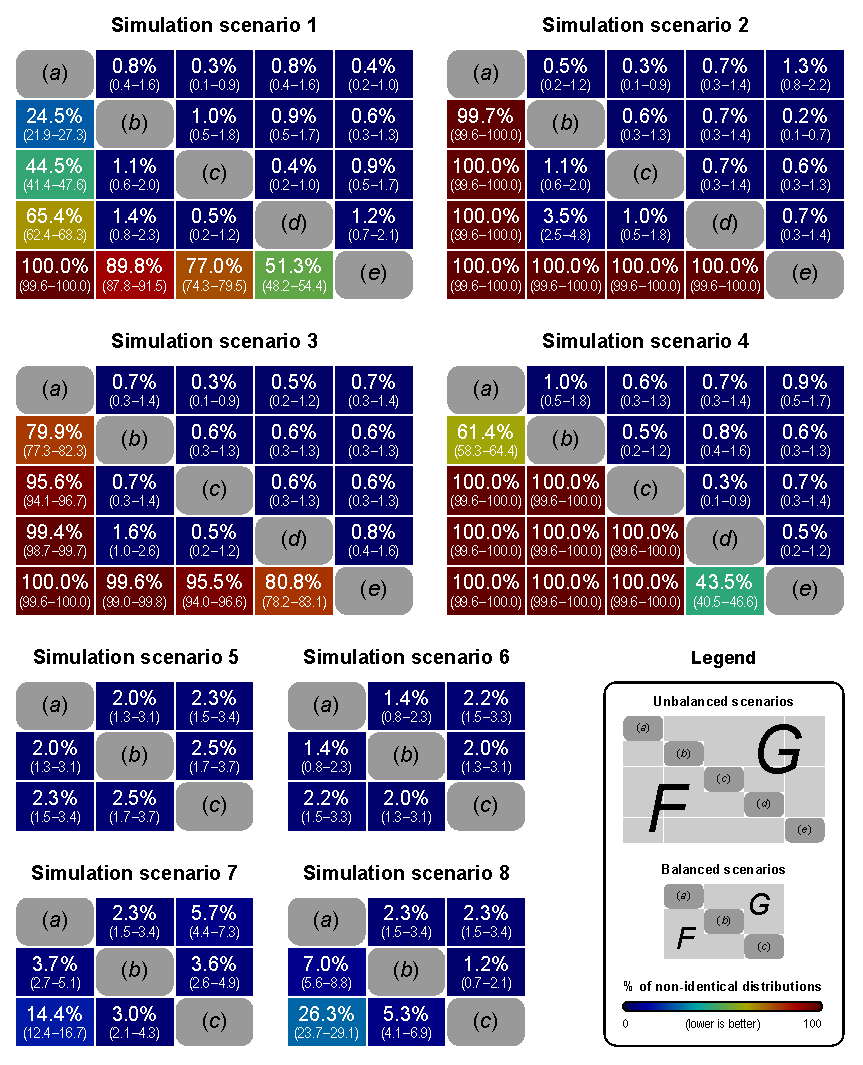
\includegraphics[width=12.6cm]{images/kolmo.eps}
\caption[Heatmaps for evaluation of pivotality for $F$ and $G$ statistics.]{Heatmaps for the comparison of the distributions obtained under different variance settings for identical sample sizes. In each map, the cells below the main diagonal contain the results for the pairwise $F$ statistic, and above, for the $G$ statistic. The percentages refer to the fraction of the 1000 tests in which the distribution of the statistic for one variance setting was found different than for another in the same simulation scenario. Each variance setting is indicated by letters (\emph{a}--\emph{e}), corresponding to the same letters in Table~\ref{tab:perm:kolmo}. Smaller percentages indicate robustness of the statistic to heteroscedasticity. Confidence intervals (95\%) are shown in parenthesis.}
\label{fig:perm:kolmo}
\end{figure}

In balanced designs, either with two (simulation scenarios 5 and 6) or more (scenarios 7 and 8) groups, the $F$ statistic had a better behaviour than in unbalanced cases. For two samples of the same size, there is no difference between $F$ and $G$. For more than two groups, the $G$ statistic behaved consistently better than $F$, particularly for large variance differences.

These results suggest that the $G$ statistic is more appropriate under heteroscedasticity, with balanced or unbalanced designs, as it preserves its distributional properties, indicating more adequacy for use with neuroimaging. The $F$ statistic, on the other hand, does not preserve pivotality and can, nonetheless, be used under heteroscedasticity when the groups have the same size.

With respect to error type \textsc{i}, both $F$ and $G$ resulted in similar amount of false positives when assessed non-parametrically. The $G$ yielded generally higher power than $F$, particularly in the presence of heteroscedasticity and with unequal sample sizes. These results are presented in Table~\ref{tab:perm:comparefg}.

\begin{table}[!p]
\caption[False positive rate and power for the statistics $F$ and $G$.]{Proportion of error type I and power (\%) for the statistics $F$ and $G$ in the various simulation scenarios and variance configurations shown in Table~\ref{tab:perm:kolmo}. Confidence intervals (95\%) are shown in parenthesis.}
\begin{center}
{\small
\begin{tabular}{@{}m{18mm}<{\raggedright}m{8mm}<{\centering}m{20mm}<{\centering}m{20mm}<{\centering}m{20mm}<{\centering}m{20mm}<{\centering}@{}}
\toprule
\multirow{2}{*}{\parbox{18mm}{\vspace{4pt}Simulation scenario}} &\multirow{2}{*}{\raisebox{-2pt}{$\star$}} & \multicolumn{2}{c}{Proportion of error type \textsc{i}} & \multicolumn{2}{c}{Power}\\
\cmidrule(lr){3-4} \cmidrule(l){5-6}
{} & {} & $F$ & $G$ & $F$ & $G$\\
\midrule
\multirow{5}{*}{1} & (\emph{a}) & 5.9 \scalebox{.7}[1.0]{(4.6--7.5)} & 6.1 \scalebox{.7}[1.0]{(4.8--7.8)} & 20.1 \scalebox{.7}[1.0]{(17.7--22.7)} & 23.8 \scalebox{.7}[1.0]{(21.3--26.5)}\\
{}                 & (\emph{b}) & 4.9 \scalebox{.7}[1.0]{(3.7--6.4)} & 5.3 \scalebox{.7}[1.0]{(4.1--6.9)} & 28.3 \scalebox{.7}[1.0]{(25.6--31.2)} & 31.9 \scalebox{.7}[1.0]{(29.1--34.9)}\\
{}                 & (\emph{c}) & 4.7 \scalebox{.7}[1.0]{(3.6--6.2)} & 4.5 \scalebox{.7}[1.0]{(3.4--6.0)} & 29.3 \scalebox{.7}[1.0]{(26.6--32.2)} & 32.6 \scalebox{.7}[1.0]{(29.8--35.6)}\\
{}                 & (\emph{d}) & 4.9 \scalebox{.7}[1.0]{(3.7--6.4)} & 4.6 \scalebox{.7}[1.0]{(3.5--6.1)} & 29.9 \scalebox{.7}[1.0]{(27.1--32.8)} & 32.0 \scalebox{.7}[1.0]{(29.2--35.0)}\\
{}                 & (\emph{e}) & 3.9 \scalebox{.7}[1.0]{(2.9--5.3)} & 4.1 \scalebox{.7}[1.0]{(3.0--5.5)} & 14.0 \scalebox{.7}[1.0]{(12.0--16.3)} & 14.1 \scalebox{.7}[1.0]{(12.1--16.4)}\\
\midrule
\multirow{5}{*}{2} & (\emph{a}) & 6.7 \scalebox{.7}[1.0]{(5.3--8.4)} & 6.6 \scalebox{.7}[1.0]{(5.2--8.3)} & 29.1 \scalebox{.7}[1.0]{(26.4--32.0)} & 38.3 \scalebox{.7}[1.0]{(35.3--41.4)}\\
{}                 & (\emph{b}) & 5.0 \scalebox{.7}[1.0]{(3.8--6.5)} & 4.6 \scalebox{.7}[1.0]{(3.5--6.1)} & 42.4 \scalebox{.7}[1.0]{(39.4--45.5)} & 48.8 \scalebox{.7}[1.0]{(45.7--51.9)}\\
{}                 & (\emph{c}) & 5.0 \scalebox{.7}[1.0]{(3.8--6.5)} & 5.8 \scalebox{.7}[1.0]{(4.5--7.4)} & 44.6 \scalebox{.7}[1.0]{(41.6--47.7)} & 48.9 \scalebox{.7}[1.0]{(45.8--52.0)}\\
{}                 & (\emph{d}) & 6.1 \scalebox{.7}[1.0]{(4.8--7.8)} & 6.2 \scalebox{.7}[1.0]{(4.9--7.9)} & 42.3 \scalebox{.7}[1.0]{(39.3--45.4)} & 46.7 \scalebox{.7}[1.0]{(43.6--49.8)}\\
{}                 & (\emph{e}) & 5.9 \scalebox{.7}[1.0]{(4.6--7.5)} & 6.2 \scalebox{.7}[1.0]{(4.9--7.9)} & 19.5 \scalebox{.7}[1.0]{(17.2--22.1)} & 19.0 \scalebox{.7}[1.0]{(16.7--21.6)}\\
\midrule
\multirow{5}{*}{3} & (\emph{a}) & 5.2 \scalebox{.7}[1.0]{(4.0--6.8)} & 5.0 \scalebox{.7}[1.0]{(3.8--6.5)} & 90.4 \scalebox{.7}[1.0]{(88.4--92.1)} & 92.3 \scalebox{.7}[1.0]{(90.5--93.8)}\\
{}                 & (\emph{b}) & 4.9 \scalebox{.7}[1.0]{(3.7--6.4)} & 5.1 \scalebox{.7}[1.0]{(3.9--6.6)} & 99.7 \scalebox{.7}[1.0]{(99.1--99.9)} & 99.8 \scalebox{.7}[1.0]{(99.3--100)}\\
{}                 & (\emph{c}) & 6.3 \scalebox{.7}[1.0]{(5.0--8.0)} & 6.2 \scalebox{.7}[1.0]{(4.9--7.9)} & 99.8 \scalebox{.7}[1.0]{(99.3--100)}  & 99.8 \scalebox{.7}[1.0]{(99.3--100)}\\
{}                 & (\emph{d}) & 4.4 \scalebox{.7}[1.0]{(3.3--5.9)} & 4.4 \scalebox{.7}[1.0]{(3.3--5.9)} & 99.6 \scalebox{.7}[1.0]{(99.0--99.8)} & 99.6 \scalebox{.7}[1.0]{(99.0--99.8)}\\
{}                 & (\emph{e}) & 4.4 \scalebox{.7}[1.0]{(3.3--5.9)} & 4.4 \scalebox{.7}[1.0]{(3.3--5.9)} & 72.9 \scalebox{.7}[1.0]{(70.1--75.6)} & 72.9 \scalebox{.7}[1.0]{(70.1--75.6)}\\
\midrule
\multirow{5}{*}{4} & (\emph{a}) & 6.4 \scalebox{.7}[1.0]{(5.0--8.1)} & 5.7 \scalebox{.7}[1.0]{(4.4--7.3)} & 10.2 \scalebox{.7}[1.0]{(8.5--12.2)}  & 19.4 \scalebox{.7}[1.0]{(17.1--22.0)}\\
{}                 & (\emph{b}) & 5.3 \scalebox{.7}[1.0]{(4.1--6.9)} & 5.6 \scalebox{.7}[1.0]{(4.3--7.2)} & 37.8 \scalebox{.7}[1.0]{(34.9--40.9)} & 45.6 \scalebox{.7}[1.0]{(42.5--48.7)}\\
{}                 & (\emph{c}) & 5.7 \scalebox{.7}[1.0]{(4.4--7.3)} & 4.9 \scalebox{.7}[1.0]{(3.7--6.4)} & 72.2 \scalebox{.7}[1.0]{(69.3--74.9)} & 74.9 \scalebox{.7}[1.0]{(72.1--77.5)}\\
{}                 & (\emph{d}) & 3.1 \scalebox{.7}[1.0]{(2.2--4.4)} & 3.7 \scalebox{.7}[1.0]{(2.7--5.1)} & 34.6 \scalebox{.7}[1.0]{(31.7--37.6)} & 44.6 \scalebox{.7}[1.0]{(41.6--47.7)}\\
{}                 & (\emph{e}) & 4.5 \scalebox{.7}[1.0]{(3.4--6.0)} & 4.2 \scalebox{.7}[1.0]{(3.1--5.6)} &  9.7 \scalebox{.7}[1.0]{(8.0--11.7)}  & 15.7 \scalebox{.7}[1.0]{(13.6--18.1)}\\
\midrule
\multirow{3}{*}{5} & (\emph{a}) & 4.3 \scalebox{.7}[1.0]{(3.2--5.7)} & 4.3 \scalebox{.7}[1.0]{(3.2--5.7)} & 29.9 \scalebox{.7}[1.0]{(27.1--32.8)} & 29.9 \scalebox{.7}[1.0]{(27.1--32.8)}\\
{}                 & (\emph{b}) & 4.3 \scalebox{.7}[1.0]{(3.2--5.7)} & 4.3 \scalebox{.7}[1.0]{(3.2--5.7)} & 30.6 \scalebox{.7}[1.0]{(27.8--33.5)} & 30.6 \scalebox{.7}[1.0]{(27.8--33.5)}\\
{}                 & (\emph{c}) & 6.9 \scalebox{.7}[1.0]{(5.5--8.6)} & 6.9 \scalebox{.7}[1.0]{(5.5--8.6)} & 14.5 \scalebox{.7}[1.0]{(12.5--16.8)} & 14.5 \scalebox{.7}[1.0]{(12.5--16.8)}\\
\midrule
\multirow{3}{*}{6} & (\emph{a}) & 3.3 \scalebox{.7}[1.0]{(2.4--4.6)} & 3.3 \scalebox{.7}[1.0]{(2.4--4.6)} & 92.6 \scalebox{.7}[1.0]{(90.8--94.1)} & 92.6 \scalebox{.7}[1.0]{(90.8--94.1)}\\
{}                 & (\emph{b}) & 4.4 \scalebox{.7}[1.0]{(3.3--5.9)} & 4.4 \scalebox{.7}[1.0]{(3.3--5.9)} & 90.5 \scalebox{.7}[1.0]{(88.5--92.2)} & 90.5 \scalebox{.7}[1.0]{(88.5--92.2)}\\
{}                 & (\emph{c}) & 4.4 \scalebox{.7}[1.0]{(3.3--5.9)} & 4.4 \scalebox{.7}[1.0]{(3.3--5.9)} & 53.7 \scalebox{.7}[1.0]{(50.6--56.8)} & 53.7 \scalebox{.7}[1.0]{(50.6--56.8)}\\
\midrule
\multirow{3}{*}{7} & (\emph{a}) & 5.6 \scalebox{.7}[1.0]{(4.3--7.2)} & 5.5 \scalebox{.7}[1.0]{(4.3--7.1)} & 11.0 \scalebox{.7}[1.0]{(9.2--13.1)}  &  8.8 \scalebox{.7}[1.0]{(7.2--10.7)}\\
{}                 & (\emph{b}) & 5.2 \scalebox{.7}[1.0]{(4.0--6.8)} & 4.4 \scalebox{.7}[1.0]{(3.3--5.9)} &  6.5 \scalebox{.7}[1.0]{(5.1--8.2)}   &  7.8 \scalebox{.7}[1.0]{(6.3--9.6)}\\
{}                 & (\emph{c}) & 5.7 \scalebox{.7}[1.0]{(4.4--7.3)} & 4.8 \scalebox{.7}[1.0]{(3.6--6.3)} &  5.8 \scalebox{.7}[1.0]{(4.5--7.4)}   &  6.9 \scalebox{.7}[1.0]{(5.5--8.6)}\\
\midrule
\multirow{3}{*}{8} & (\emph{a}) & 4.6 \scalebox{.7}[1.0]{(3.5--6.1)} & 4.5 \scalebox{.7}[1.0]{(3.4--6.0)} & 78.7 \scalebox{.7}[1.0]{(76.1--81.1)} & 78.1 \scalebox{.7}[1.0]{(75.4--80.6)}\\
{}                 & (\emph{b}) & 4.6 \scalebox{.7}[1.0]{(3.5--6.1)} & 5.6 \scalebox{.7}[1.0]{(4.3--7.2)} & 40.7 \scalebox{.7}[1.0]{(37.7--43.8)} & 45.5 \scalebox{.7}[1.0]{(42.4--48.6)}\\
{}                 & (\emph{c}) & 4.7 \scalebox{.7}[1.0]{(3.6--6.2)} & 4.8 \scalebox{.7}[1.0]{(3.6--6.3)} & 11.6 \scalebox{.7}[1.0]{(9.8--13.7)}  & 19.3 \scalebox{.7}[1.0]{(17.0--21.9)}\\
\bottomrule
\end{tabular}}
\end{center}
\label{tab:perm:comparefg}
\end{table}

\subsection{Permutation strategies}
\label{sec:perm:results_perm}

The different simulation parameters allowed 1536 different regression scenarios, being 768 without signal and 768 with signal; a summary is shown in Table~\ref{tab:perm:summary}, and some of the most representative in Table~\ref{tab:perm:methods_resultsC}. In ``well behaved'' scenarios, i.e., large number of observations, orthogonal regressors and normally distributed errors, all methods tended to behave generally well, with adequate control over type~\textsc{i} error and fairly similar power. However, performance differences between the permutation strategies shown in Table~\ref{tab:perm:methods} became more noticeable as the sample sizes were decreased and skewed errors were introduced.

\begin{table}[!tp]
\caption[Summary of the amount of error type \textsc{i} and power for the different permutation strategies.]{A summary of the results for the 1536 simulations with different parameters. The amount of error type \textsc{i} is calculated for the 768 simulations without signal ($\beta_1$ = 0), whereas the power was calculated for the remaining 768 simulations with signal ($\beta_1$ = 0.5). Confidence intervals (\textsc{ci}) are at 95\%.}
\begin{center}
{\small
\begin{tabular}{@{}m{37mm}<{\raggedright}m{18mm}<{\centering}m{18mm}<{\centering}m{18mm}<{\centering}m{18mm}<{\centering}@{}}
\toprule
\multirow{2}{*}{\raisebox{-3pt}{Method}} &   \multicolumn{3}{c}{Proportion of error type \textsc{i}} & \multirow{2}{19mm}{\raisebox{-3pt}{Average} power}\\
\cmidrule(lr){2-4}
                        & Within \textsc{ci} & Below \textsc{ci} & Above \textsc{ci}\\
\midrule
Draper--Stoneman & 86.33\% &  8.20\% &  5.47\% & 72.96\%\\
Still--White     & 67.84\% & 14.58\% & 17.58\% & 71.82\%\\
Freedman--Lane   & 88.67\% &  8.46\% &  2.86\% & 73.09\%\\
ter Braak        & 83.59\% & 11.07\% &  5.34\% & 73.38\%\\
Kennedy          & 77.60\% &  1.04\% & 21.35\% & 74.81\%\\
Manly            & 73.31\% & 15.89\% & 10.81\% & 73.38\%\\
Smith            & 89.32\% &  7.81\% &  2.86\% & 72.90\%\\
Huh--Jhun        & 85.81\% &  9.24\% &  4.95\% & 71.62\%\\
Parametric       & 77.47\% & 14.84\% &  7.68\% & 72.73\%\\
\bottomrule
\end{tabular}}
\end{center}
{\footnotesize
When the amount of errors is below the nominal level (here, $\alpha=0.05)$, the test is said to be \emph{conservative}. If above, it is \emph{invalid}.\par}
\label{tab:perm:summary}
\end{table}

\begin{table}[b!]
\caption[Amount of error type \textsc{i} for representative simulation scenarios.]{\emph{(Page \pageref{tab:perm:methods_resultsT})} Proportion of error type \textsc{i} (for $\alpha$ = 0.05), for some representative of the 768 simulation scenarios that did not have signal, using the different permutation methods, and with $G$ as the statistic in the absence of \textsc{eb} (so, equivalent to the $F$ statistic). Confidence intervals (95\%) are shown in parenthesis.}
{\footnotesize
$N$: number of observations;
$\mathbf{x}_1$ and $\mathbf{z}_1$: regressors of interest and of no interest, respectively, being either continuous (\textsc{c}) or discrete (\textsc{d}).
$\rho$: correlation between $\mathbf{x}_1$ and $\mathbf{z}_1$;
\raisebox{-1pt}{\ding{'42}}: model partitioned or not (using the \citet{Beckmann2001} scheme, shown in \ref{sec:perm:partitioning});
$\mathbf{\epsilon}$: distribution of the simulated errors, which can be normal ($\mathcal{N}$), uniform ($\mathcal{U}$), exponential ($\mathcal{E}$) or Weibull ($\mathcal{W}$);
\textsc{ee}: errors treated as exchangeable;
\textsc{ise}: errors treated as independent and symmetric.
The methods are the same shown in Table~\ref{tab:perm:methods}: Draper--Stoneman (D--S), Still--White (S--W), Freedman--Lane (F--L), ter Braak (tB), Kennedy (K), Manly (M), Huh--Jhun (H--J), Smith (S) and parametric (P), the last not using permutations.
\par}
\label{tab:perm:methods_resultsC}
\end{table}


\begin{sidewaystable}
\begin{center}
{\footnotesize
\begin{tabular}{@{}c@{\hspace{2.5mm}}c@{\hspace{2.5mm}}c@{\hspace{2.5mm}}c@{\hspace{2.5mm}}c@{\hspace{2.5mm}}c@{\hspace{2.5mm}}c@{\hspace{2.5mm}}c@{\hspace{2.5mm}}c@{\hspace{3mm}}c@{\hspace{3mm}}c@{\hspace{3mm}}c@{\hspace{3mm}}c@{\hspace{3mm}}c@{\hspace{3mm}}c@{\hspace{3mm}}c@{\hspace{3mm}}c@{}}
\toprule
\multicolumn{8}{c}{Simulation parameters} & \multicolumn{9}{c}{Proportion of error type \textsc{i} (\%)}\\
\cmidrule(r){1-8}\cmidrule(l){9-17}
$N$ & $\mathbf{x}_1$ & $\mathbf{z}_1$ & $\rho$ & \raisebox{-1pt}{\ding{'42}} & $\boldsymbol{\epsilon}$ & \textsc{ee} & \textsc{ise} & D--S & S--W & F--L & tB & K & M & S & H--J & P \\
\midrule
12 & \textsc{c} & \textsc{c} & 0   & \ding{'67} & $\mathcal{N}$ & \ding{'63} & \ding{'67} & 4.9 \scalebox{.7}[1.0]{(3.7--6.4)} & 5.3 \scalebox{.7}[1.0]{(4.1--6.9)} & 5.1 \scalebox{.7}[1.0]{(3.9--6.6)} & 5.3 \scalebox{.7}[1.0]{(4.1--6.9)} & 5.3 \scalebox{.7}[1.0]{(4.1--6.9)} & 5.0 \scalebox{.7}[1.0]{(3.8--6.5)} & 4.9 \scalebox{.7}[1.0]{(3.7--6.4)} & 4.7 \scalebox{.7}[1.0]{(3.6--6.2)} & 4.4 \scalebox{.7}[1.0]{(3.3--5.9)}\\
12 & \textsc{c} & \textsc{c} & 0   & \ding{'67} & $\mathcal{U}$ & \ding{'63} & \ding{'63} & 5.3 \scalebox{.7}[1.0]{(4.1--6.9)} & 6.9 \scalebox{.7}[1.0]{(5.5--8.6)} & 5.1 \scalebox{.7}[1.0]{(3.9--6.6)} & 5.2 \scalebox{.7}[1.0]{(4.0--6.8)} & 6.9 \scalebox{.7}[1.0]{(5.5--8.6)} & 5.8 \scalebox{.7}[1.0]{(4.5--7.4)} & 5.3 \scalebox{.7}[1.0]{(4.1--6.9)} & 5.2 \scalebox{.7}[1.0]{(4.0--6.8)} & 4.6 \scalebox{.7}[1.0]{(3.5--6.1)}\\
12 & \textsc{c} & \textsc{c} & 0   & \ding{'67} & $\mathcal{W}$ & \ding{'63} & \ding{'67} & 5.9 \scalebox{.7}[1.0]{(4.6--7.5)} & 6.5 \scalebox{.7}[1.0]{(5.1--8.2)} & 5.2 \scalebox{.7}[1.0]{(4.0--6.8)} & 5.4 \scalebox{.7}[1.0]{(4.2--7.0)} & 6.5 \scalebox{.7}[1.0]{(5.1--8.2)} & 5.0 \scalebox{.7}[1.0]{(3.8--6.5)} & 5.9 \scalebox{.7}[1.0]{(4.6--7.5)} & 5.4 \scalebox{.7}[1.0]{(4.2--7.0)} & 8.3 \scalebox{.7}[1.0]{(6.7--10.2)}\\
12 & \textsc{c} & \textsc{c} & 0   & \ding{'67} & $\mathcal{E}$ & \ding{'63} & \ding{'63} & 5.3 \scalebox{.7}[1.0]{(4.1--6.9)} & 6.9 \scalebox{.7}[1.0]{(5.5--8.6)} & 5.1 \scalebox{.7}[1.0]{(3.9--6.6)} & 4.7 \scalebox{.7}[1.0]{(3.6--6.2)} & 6.9 \scalebox{.7}[1.0]{(5.5--8.6)} & 5.0 \scalebox{.7}[1.0]{(3.8--6.5)} & 5.3 \scalebox{.7}[1.0]{(4.1--6.9)} & 4.8 \scalebox{.7}[1.0]{(3.6--6.3)} & 5.7 \scalebox{.7}[1.0]{(4.4--7.3)}\\
12 & \textsc{c} & \textsc{c} & 0.8 & \ding{'67} & $\mathcal{N}$ & \ding{'63} & \ding{'67} & 4.4 \scalebox{.7}[1.0]{(3.3--5.9)} & 3.6 \scalebox{.7}[1.0]{(2.6--4.9)} & 5.1 \scalebox{.7}[1.0]{(3.9--6.6)} & 5.2 \scalebox{.7}[1.0]{(4.0--6.8)} & 5.8 \scalebox{.7}[1.0]{(4.5--7.4)} & 4.8 \scalebox{.7}[1.0]{(3.6--6.3)} & 5.1 \scalebox{.7}[1.0]{(3.9--6.6)} & 4.4 \scalebox{.7}[1.0]{(3.3--5.9)} & 4.4 \scalebox{.7}[1.0]{(3.3--5.9)}\\
12 & \textsc{c} & \textsc{c} & 0.8 & \ding{'67} & $\mathcal{W}$ & \ding{'63} & \ding{'67} & 1.5 \scalebox{.7}[1.0]{(0.9--2.5)} & 1.2 \scalebox{.7}[1.0]{(0.7--2.1)} & 4.8 \scalebox{.7}[1.0]{(3.6--6.3)} & 5.2 \scalebox{.7}[1.0]{(4.0--6.8)} & 6.5 \scalebox{.7}[1.0]{(5.1--8.2)} & 4.9 \scalebox{.7}[1.0]{(3.7--6.4)} & 5.8 \scalebox{.7}[1.0]{(4.5--7.4)} & 5.8 \scalebox{.7}[1.0]{(4.5--7.4)} & 8.5 \scalebox{.7}[1.0]{(6.9--10.4)}\\
12 & \textsc{c} & \textsc{c} & 0.8 & \ding{'67} & $\mathcal{N}$ & \ding{'63} & \ding{'63} & 5.5 \scalebox{.7}[1.0]{(4.2--7.1)} & 5.4 \scalebox{.7}[1.0]{(4.2--7.0)} & 4.9 \scalebox{.7}[1.0]{(3.7--6.4)} & 5.4 \scalebox{.7}[1.0]{(4.2--7.0)} & 7.5 \scalebox{.7}[1.0]{(6.0--9.3)} & 4.8 \scalebox{.7}[1.0]{(3.6--6.3)} & 4.8 \scalebox{.7}[1.0]{(3.6--6.3)} & 5.8 \scalebox{.7}[1.0]{(4.5--7.4)} & 4.6 \scalebox{.7}[1.0]{(3.5--6.1)}\\
12 & \textsc{c} & \textsc{c} & 0.8 & \ding{'63} & $\mathcal{N}$ & \ding{'63} & \ding{'63} & 5.1 \scalebox{.7}[1.0]{(3.9--6.6)} & 7.2 \scalebox{.7}[1.0]{(5.8--9.0)} & 5.4 \scalebox{.7}[1.0]{(4.2--7.0)} & 4.3 \scalebox{.7}[1.0]{(3.2--5.7)} & 7.2 \scalebox{.7}[1.0]{(5.8--9.0)} & 5.2 \scalebox{.7}[1.0]{(4.0--6.8)} & 5.1 \scalebox{.7}[1.0]{(3.9--6.6)} & 4.6 \scalebox{.7}[1.0]{(3.5--6.1)} & 4.6 \scalebox{.7}[1.0]{(3.5--6.1)}\\
12 & \textsc{c} & \textsc{d} & 0   & \ding{'67} & $\mathcal{W}$ & \ding{'63} & \ding{'67} & 5.6 \scalebox{.7}[1.0]{(4.3--7.2)} & 6.8 \scalebox{.7}[1.0]{(5.4--8.5)} & 5.4 \scalebox{.7}[1.0]{(4.2--7.0)} & 4.7 \scalebox{.7}[1.0]{(3.6--6.2)} & 6.8 \scalebox{.7}[1.0]{(5.4--8.5)} & 4.0 \scalebox{.7}[1.0]{(3.0--5.4)} & 5.6 \scalebox{.7}[1.0]{(4.3--7.2)} & 3.7 \scalebox{.7}[1.0]{(2.7--5.1)} & 8.9 \scalebox{.7}[1.0]{(7.3--10.8)}\\
12 & \textsc{c} & \textsc{d} & 0   & \ding{'67} & $\mathcal{N}$ & \ding{'63} & \ding{'67} & 3.9 \scalebox{.7}[1.0]{(2.9--5.3)} & 4.9 \scalebox{.7}[1.0]{(3.7--6.4)} & 3.9 \scalebox{.7}[1.0]{(2.9--5.3)} & 4.0 \scalebox{.7}[1.0]{(3.0--5.4)} & 4.9 \scalebox{.7}[1.0]{(3.7--6.4)} & 4.3 \scalebox{.7}[1.0]{(3.2--5.7)} & 3.9 \scalebox{.7}[1.0]{(2.9--5.3)} & 4.2 \scalebox{.7}[1.0]{(3.1--5.6)} & 3.7 \scalebox{.7}[1.0]{(2.7--5.1)}\\
12 & \textsc{c} & \textsc{d} & 0   & \ding{'67} & $\mathcal{W}$ & \ding{'67} & \ding{'63} & 2.9 \scalebox{.7}[1.0]{(2.0--4.1)} & 4.3 \scalebox{.7}[1.0]{(3.2--5.7)} & 2.6 \scalebox{.7}[1.0]{(1.8--3.8)} & 2.8 \scalebox{.7}[1.0]{(1.9--4.0)} & 4.3 \scalebox{.7}[1.0]{(3.2--5.7)} & 14.1 \scalebox{.7}[1.0]{(12.1--16.4)} & 2.9 \scalebox{.7}[1.0]{(2.0--4.1)} & 16.4 \scalebox{.7}[1.0]{(14.2--18.8)} & 9.0 \scalebox{.7}[1.0]{(7.4--10.9)}\\
12 & \textsc{d} & \textsc{d} & 0   & \ding{'67} & $\mathcal{W}$ & \ding{'63} & \ding{'67} & 3.2 \scalebox{.7}[1.0]{(2.3--4.5)} & 4.6 \scalebox{.7}[1.0]{(3.5--6.1)} & 2.2 \scalebox{.7}[1.0]{(1.5--3.3)} & 2.0 \scalebox{.7}[1.0]{(1.3--3.1)} & 4.6 \scalebox{.7}[1.0]{(3.5--6.1)} & 3.8 \scalebox{.7}[1.0]{(2.8--5.2)} & 3.2 \scalebox{.7}[1.0]{(2.3--4.5)} & 2.6 \scalebox{.7}[1.0]{(1.8--3.8)} & 0.5 \scalebox{.7}[1.0]{(0.2--1.2)}\\
24 & \textsc{c} & \textsc{c} & 0.8 & \ding{'67} & $\mathcal{N}$ & \ding{'63} & \ding{'67} & 4.4 \scalebox{.7}[1.0]{(3.3--5.9)} & 3.5 \scalebox{.7}[1.0]{(2.5--4.8)} & 4.3 \scalebox{.7}[1.0]{(3.2--5.7)} & 4.4 \scalebox{.7}[1.0]{(3.3--5.9)} & 4.9 \scalebox{.7}[1.0]{(3.7--6.4)} & 4.4 \scalebox{.7}[1.0]{(3.3--5.9)} & 4.3 \scalebox{.7}[1.0]{(3.2--5.7)} & 4.5 \scalebox{.7}[1.0]{(3.4--6.0)} & 4.4 \scalebox{.7}[1.0]{(3.3--5.9)}\\
24 & \textsc{d} & \textsc{d} & 0   & \ding{'67} & $\mathcal{N}$ & \ding{'63} & \ding{'67} & 5.0 \scalebox{.7}[1.0]{(3.8--6.5)} & 5.4 \scalebox{.7}[1.0]{(4.2--7.0)} & 5.1 \scalebox{.7}[1.0]{(3.9--6.6)} & 5.1 \scalebox{.7}[1.0]{(3.9--6.6)} & 5.4 \scalebox{.7}[1.0]{(4.2--7.0)} & 4.9 \scalebox{.7}[1.0]{(3.7--6.4)} & 5.0 \scalebox{.7}[1.0]{(3.8--6.5)} & 4.5 \scalebox{.7}[1.0]{(3.4--6.0)} & 5.0 \scalebox{.7}[1.0]{(3.8--6.5)}\\
24 & \textsc{d} & \textsc{d} & 0   & \ding{'67} & $\mathcal{U}$ & \ding{'63} & \ding{'67} & 6.2 \scalebox{.7}[1.0]{(4.9--7.9)} & 6.6 \scalebox{.7}[1.0]{(5.2--8.3)} & 6.3 \scalebox{.7}[1.0]{(5.0--8.0)} & 5.9 \scalebox{.7}[1.0]{(4.6--7.5)} & 6.6 \scalebox{.7}[1.0]{(5.2--8.3)} & 5.5 \scalebox{.7}[1.0]{(4.2--7.1)} & 6.2 \scalebox{.7}[1.0]{(4.9--7.9)} & 5.9 \scalebox{.7}[1.0]{(4.6--7.5)} & 5.8 \scalebox{.7}[1.0]{(4.5--7.4)}\\
24 & \textsc{d} & \textsc{d} & 0.8 & \ding{'67} & $\mathcal{U}$ & \ding{'63} & \ding{'67} & 4.9 \scalebox{.7}[1.0]{(3.7--6.4)} & 1.8 \scalebox{.7}[1.0]{(1.1--2.8)} & 5.1 \scalebox{.7}[1.0]{(3.9--6.6)} & 4.8 \scalebox{.7}[1.0]{(3.6--6.3)} & 5.4 \scalebox{.7}[1.0]{(4.2--7.0)} & 5.1 \scalebox{.7}[1.0]{(3.9--6.6)} & 5.2 \scalebox{.7}[1.0]{(4.0--6.8)} & 5.7 \scalebox{.7}[1.0]{(4.4--7.3)} & 5.4 \scalebox{.7}[1.0]{(4.2--7.0)}\\
48 & \textsc{c} & \textsc{c} & 0   & \ding{'67} & $\mathcal{N}$ & \ding{'67} & \ding{'63} & 4.9 \scalebox{.7}[1.0]{(3.7--6.4)} & 5.4 \scalebox{.7}[1.0]{(4.2--7.0)} & 5.0 \scalebox{.7}[1.0]{(3.8--6.5)} & 5.6 \scalebox{.7}[1.0]{(4.3--7.2)} & 5.4 \scalebox{.7}[1.0]{(4.2--7.0)} & 3.8 \scalebox{.7}[1.0]{(2.8--5.2)} & 4.9 \scalebox{.7}[1.0]{(3.7--6.4)} & 6.0 \scalebox{.7}[1.0]{(4.7--7.6)} & 5.0 \scalebox{.7}[1.0]{(3.8--6.5)}\\
48 & \textsc{c} & \textsc{c} & 0.8 & \ding{'63} & $\mathcal{U}$ & \ding{'63} & \ding{'67} & 5.1 \scalebox{.7}[1.0]{(3.9--6.6)} & 5.4 \scalebox{.7}[1.0]{(4.2--7.0)} & 5.0 \scalebox{.7}[1.0]{(3.8--6.5)} & 5.7 \scalebox{.7}[1.0]{(4.4--7.3)} & 5.4 \scalebox{.7}[1.0]{(4.2--7.0)} & 5.2 \scalebox{.7}[1.0]{(4.0--6.8)} & 5.1 \scalebox{.7}[1.0]{(3.9--6.6)} & 5.6 \scalebox{.7}[1.0]{(4.3--7.2)} & 5.6 \scalebox{.7}[1.0]{(4.3--7.2)}\\
48 & \textsc{c} & \textsc{c} & 0.8 & \ding{'63} & $\mathcal{N}$ & \ding{'63} & \ding{'67} & 4.6 \scalebox{.7}[1.0]{(3.5--6.1)} & 4.8 \scalebox{.7}[1.0]{(3.6--6.3)} & 4.7 \scalebox{.7}[1.0]{(3.6--6.2)} & 4.7 \scalebox{.7}[1.0]{(3.6--6.2)} & 4.8 \scalebox{.7}[1.0]{(3.6--6.3)} & 4.6 \scalebox{.7}[1.0]{(3.5--6.1)} & 4.6 \scalebox{.7}[1.0]{(3.5--6.1)} & 4.4 \scalebox{.7}[1.0]{(3.3--5.9)} & 4.5 \scalebox{.7}[1.0]{(3.4--6.0)}\\
48 & \textsc{c} & \textsc{d} & 0   & \ding{'67} & $\mathcal{E}$ & \ding{'67} & \ding{'63} & 5.4 \scalebox{.7}[1.0]{(4.2--7.0)} & 5.7 \scalebox{.7}[1.0]{(4.4--7.3)} & 5.1 \scalebox{.7}[1.0]{(3.9--6.6)} & 5.5 \scalebox{.7}[1.0]{(4.2--7.1)} & 5.7 \scalebox{.7}[1.0]{(4.4--7.3)} & 9.2 \scalebox{.7}[1.0]{(7.6--11.2)} & 5.4 \scalebox{.7}[1.0]{(4.2--7.0)} & 4.3 \scalebox{.7}[1.0]{(3.2--5.7)} & 5.1 \scalebox{.7}[1.0]{(3.9--6.6)}\\
48 & \textsc{c} & \textsc{d} & 0.8 & \ding{'67} & $\mathcal{E}$ & \ding{'63} & \ding{'67} & 5.5 \scalebox{.7}[1.0]{(4.2--7.1)} & 0.3 \scalebox{.7}[1.0]{(0.1--0.9)} & 5.0 \scalebox{.7}[1.0]{(3.8--6.5)} & 5.0 \scalebox{.7}[1.0]{(3.8--6.5)} & 5.0 \scalebox{.7}[1.0]{(3.8--6.5)} & 4.9 \scalebox{.7}[1.0]{(3.7--6.4)} & 5.0 \scalebox{.7}[1.0]{(3.8--6.5)} & 5.0 \scalebox{.7}[1.0]{(3.8--6.5)} & 4.9 \scalebox{.7}[1.0]{(3.7--6.4)}\\
96 & \textsc{c} & \textsc{c} & 0   & \ding{'67} & $\mathcal{N}$ & \ding{'63} & \ding{'63} & 5.1 \scalebox{.7}[1.0]{(3.9--6.6)} & 5.3 \scalebox{.7}[1.0]{(4.1--6.9)} & 5.1 \scalebox{.7}[1.0]{(3.9--6.6)} & 4.9 \scalebox{.7}[1.0]{(3.7--6.4)} & 5.3 \scalebox{.7}[1.0]{(4.1--6.9)} & 4.6 \scalebox{.7}[1.0]{(3.5--6.1)} & 5.1 \scalebox{.7}[1.0]{(3.9--6.6)} & 5.3 \scalebox{.7}[1.0]{(4.1--6.9)} & 4.9 \scalebox{.7}[1.0]{(3.7--6.4)}\\
96 & \textsc{c} & \textsc{c} & 0.8 & \ding{'67} & $\mathcal{N}$ & \ding{'67} & \ding{'63} & 5.0 \scalebox{.7}[1.0]{(3.8--6.5)} & 3.6 \scalebox{.7}[1.0]{(2.6--4.9)} & 5.0 \scalebox{.7}[1.0]{(3.8--6.5)} & 4.8 \scalebox{.7}[1.0]{(3.6--6.3)} & 5.2 \scalebox{.7}[1.0]{(4.0--6.8)} & 4.4 \scalebox{.7}[1.0]{(3.3--5.9)} & 5.1 \scalebox{.7}[1.0]{(3.9--6.6)} & 5.2 \scalebox{.7}[1.0]{(4.0--6.8)} & 4.9 \scalebox{.7}[1.0]{(3.7--6.4)}\\
96 & \textsc{d} & \textsc{c} & 0   & \ding{'67} & $\mathcal{W}$ & \ding{'63} & \ding{'67} & 4.9 \scalebox{.7}[1.0]{(3.7--6.4)} & 5.2 \scalebox{.7}[1.0]{(4.0--6.8)} & 4.7 \scalebox{.7}[1.0]{(3.6--6.2)} & 4.8 \scalebox{.7}[1.0]{(3.6--6.3)} & 5.2 \scalebox{.7}[1.0]{(4.0--6.8)} & 4.5 \scalebox{.7}[1.0]{(3.4--6.0)} & 4.9 \scalebox{.7}[1.0]{(3.7--6.4)} & 3.9 \scalebox{.7}[1.0]{(2.9--5.3)} & 3.6 \scalebox{.7}[1.0]{(2.6--4.9)}\\
\bottomrule
\multicolumn{17}{l}{\emph{See caption on page \pageref{tab:perm:methods_resultsC}.}}
\end{tabular}}
\end{center}
\label{tab:perm:methods_resultsT}
\end{sidewaystable}

Some of the methods are identical to each other in certain circumstances. If $\mathbf{X}$ and $\mathbf{Z}$ are orthogonal, Draper--Stoneman and Smith are equivalent. Likewise under orthogonality, Still--White produces identical regression coefficients as Freedman--Lane, although the statistic will only be the same if the loss in degrees of freedom due to $\mathbf{Z}$ is taken into account, something not always possible when the data has already been residualised and no information about the original nuisance variables is available. Nonetheless, the two methods remain asymptotically equivalent as the number of observations diverges from the number of nuisance regressors.

\paragraph{Sample size} Increasing the sample size had the effect of approaching the error rate to closer to the nominal level $\alpha=0.05$ for all methods in virtually all parameter configurations. For small samples, most methods were slightly conservative, whereas Still--White and Kennedy were anticonservative and often invalid, particularly if the distributions of the errors were skewed.

\paragraph{Continuous or categorical regressors of interest} For all methods, using continuous or categorical regressors of interest did not produce remarkable differences in the observed proportions of type~\textsc{i} error, except if the distribution of the errors was skewed and sign flipping was used (in violation of assumptions), in which case Manly and Huh--Jhun methods showed erratic control over the amount of errors.

\paragraph{Continuous or categorical nuisance regressors} The presence of continuous or categorical nuisance variables did not substantially interfere with either control over error type~\textsc{i} or power, for any of the methods, except in the presence of correlated regressors.

\paragraph{Degree of non-orthogonality and partitioning} All methods provided relatively adequate control over error type~\textsc{i} in the presence of a correlated nuisance regressor, except Still--White (conservative) and Kennedy (inflated rates). The partitioning scheme mitigated the conservativeness of the former, and the anticonservativeness of the latter.

\paragraph{Distribution of the errors} Different distributions did not substantially improve or worsen error rates when using permutation alone. Still--White and Kennedy tended to fail control over error type~\textsc{i} in virtually all situations. Sign flipping alone, when used with asymmetric distributions (in violation of assumptions), required larger samples to allow approximately exact control over the amount of error type \textsc{i}. In these cases, and with small samples, the methods Draper--Stoneman, Manly and Huh--Jhun tended to display erratic behaviour, with extremes of conservativeness and anticonservativeness depending on the other simulation parameters. The same happened with the parametric method. Freedman--Lane and Smith methods, on the other hand, tended to have a relatively constant and somewhat conservative behaviour in these situations. Permutation combined with sign-flipping generally alleviated these issues where they were observed.

\vspace{10pt}

From all the methods, the Freedman--Lane and Smith were those that performed better in most cases, and with their 95\% confidence interval covering the desired error level of 0.05 more often than any of the other methods. The Still--White and Kennedy methods did not generally control the error type~\textsc{i} for most of the simulation parameters, particularly for smaller sample sizes. On the other hand, with a few exceptions, the Freedman--Lane and the Smith methods effectively controlled the error rates in most cases, even with skewed errors and sign-flipping, being, at worst, conservative or only slightly above the nominal level. All methods were, overall, similarly powerful, with only marginal differences among those that were on average valid.

\section{Discussion}

Ideally, criteria to accept or reject a given hypothesis should be sensitive to changes in the parameters of interest (powerful), and insensitive to changes in nuisance factors (robust). As pointed out long ago by \citet{Box1955}, the assumptions on which parametric tests are built are such that the first criterion is generally satisfied, albeit not necessarily the second. Many non-parametric tests, on the other hand, are constructed such that most or all these assumptions are not demanded, satisfying the second criterion, but not necessarily the first. For current applications in neuroimaging, however, this compromise between robustness and power gains new contours and a different balance. First, in neuroimaging it is necessary to address the multiple testing problem, in which one or more tests are applied to each of thousands of points (commonly voxels, vertices or faces) of the image representation of the brain. Parametric methods require the introduction of an even larger set of assumptions to deal with multiple testing. Second, different imaging modalities not necessarily follow the same set of assumptions regarding distributions under the null at each test, neither for the covariance between tests across the brain, so that those that might be acceptably used with one method, may cause others to be invalid. Third, under non-random sampling, as common in case-control studies, the very presence of the features under investigation (such as a disorder) may compromise the assumptions on which parametric tests depend. For all these reasons, parametric methods, despite common use, are more likely to fail as candidates to provide a general statistical framework for the current variety of imaging modalities for research applications, where not only the assumptions may not be met, but also where robustness may be seen as a key factor. Permutation methods are a viable alternative, flexible enough to accommodate several experimental needs. Further to all this, our simulations showed similar and sometimes higher power compared to the parametric approach.

\subsection{Permutation tests}

Permutation tests require very few assumptions about the data and, therefore, can be applied in a wider variety of situations than parametric tests. None of the most common parametric assumptions need to hold for non-parametric tests to be valid. The assumptions that are eschewed include, for instance, the need of normality for the error terms, the need of homoscedasticity and the need of random sampling. With a very basic knowledge of sample properties or of the study design, errors can be treated as exchangeable (\textsc{ee}) and/or independent and symmetric (\textsc{ise}) and inferences that otherwise would not be possible with parametric methods become feasible. Furthermore, permutation tests permit the use of the very same regression and hypothesis testing framework, even with disparate imaging modalities, without the need to verify the validity of parametric assumptions for each of them. The \textsc{ise} can be an alternative to \textsc{ee} when the errors themselves can be considered exchangeable, but the design is not affected by permutations, as for one-sample tests. And if the assumptions for \textsc{ee} and \textsc{ise} are both met, permutation and sign flipping can both be performed to construct the empirical distribution.

The justification for permutation tests has, moreover, more solid foundations than their parametric counterparts. While the validity of parametric tests rely on random sampling, permutation tests rely on the idea of random allocation of experimental units, with no reference to any underlying population. This aspect has a key importance in biomedical research --- including neuroimaging --- where only a small minority of studies effectively use random population sampling. Most experimental studies need to use the subjects that are available in a given area, and who accept to participate (e.g. patients of a hospital or students of an university near where the \textsc{mri} equipment is installed). True random sampling is rarely achieved in real applications because, often and for different reasons, selection criteria are not truly unbiased \citep{Ludbrook1998, Pesarin2010}. Non-parametric methods allow valid inferences to be performed in these scenarios.

\subsection{Pivotal statistics}

In addition, permutation methods have the remarkable feature of allowing the use of non-standard statistics, or for which closed mathematical forms have not been derived, even asymptotically. Statistics that can be used include, for instance, those based on ranks of observations \citep{Brunner2000, Rorden2007}, derived from regression methods other than least squares \citep{Cade1996} or that are robust to outliers \citep{Theil1950, Sen1968}. For imaging applications, statistics that can be considered include the pseudo-$t$ statistic after variance smoothing \citep{Holmes1996}, the mass of connected voxels \citep{Bullmore1999}, threshold-free cluster enhancement (\textsc{tfce}) \citep{Smith2009}, as well as cases in which the distribution of the statistic may lie in a gradient between distributions, each of them with known analytical forms, such as the distribution of surface area, as demonstrated in Chapter~\ref{sec:areal} \citep[published as][]{Winkler2012}. The only requirement, in the context of neuroimaging, is that these statistics retain their distributional properties irrespective to the (unknown) population parameters.

Indeed, a large part of the voluminous literature on statistical tests when the errors cannot be assumed to be homoscedastic is concerned with the identification of the asymptotic distribution of the statistics, its analytical form, and the consequences of experimental scenarios that include unbalancedness and/or small samples. This is true even considering that in parametric settings, the statistics are invariably chosen such that their sampling distribution is independent of underlying and unknown population parameters. Permutation tests render all these issues irrelevant, as the asymptotic properties of the distributions do not need to be ascertained. For imaging, all that is needed is that the distribution remains invariant to unknown population parameters, i.e., the statistic needs to be pivotal. Parameters of the distribution proper do not need to be known, nor the distribution needs to be characterised analytically. The proposed statistic $G$, being a generalisation over various tests that have their niche applications in parametric settings, is appropriate for use with the general linear model and with a permutation framework, for being pivotal and easily implementable using simple matrix operations. Moreover, as the simulations showed, this statistic is not less powerful than the commonly used $F$ statistic.

\subsection{Permutation strategies}

From the different permutation strategies presented in Table~\ref{tab:perm:methods}, the Freedman--Lane and the Smith methods provided the most adequate control of type~\textsc{i} error across the various simulation scenarios. This is in line with the study by \citet{Anderson1999}, who found that the Freedman--Lane method is the most accurate and powerful in various different models. The Smith method was a somewhat positive surprise, not only for the overall very good performance in our simulations, but also because this method had not been extensively evaluated in previous literature, is computationally simple, and has an intuitive appeal.

\citet{Welch1990} commented that the Freedman--Lane procedure would violate the ancillarity principle, as the permutation procedure would destroy the relationship between $\mathbf{X}$ and $\mathbf{Z}$, even if these are orthogonal. Notwithstanding, even with ancillarity violated, this and other methods perform satisfactorily well.

\citet{Freedman1983} described their method as having a ``non-stochastic'' interpretation, and so, that the computed p-value would be a descriptive statistic. On the contrary, we share the same view expressed by \citet{Anderson1999}, that the rationale for the test and the procedure effectively produces a p-value that can be interpreted as a true probability for the underlying model.

Regarding differences between the methods, and even though for this study we did not evaluate the effect of extremely strong signals or of outliers, it is worth commenting that previous research have shown that the Freedman--Lane method is relatively robust to the presence of extreme outliers, whereas the ter Braak tends to become more conservative in these cases \citep{Anderson1999}. The ter Braak method, however, was shown to be more robust to extremely strong signals in the data, situations in which signal may ``leak'' into the permutation distribution with the Freedman--Lane method \citep{Salimi-Khorshidi2011}.

It should be noted that the Still--White method, as implemented for these simulations, used for the regression the model containing only the regressors of interest when computing the statistic. as shown in Table~\ref{tab:perm:methods}. It is done in this way to emulate what probably is its more common use, i.e., rearrange the data that has already been residualised from nuisance, and when the nuisance regressors are no longer available. Had the full model been used when computing the statistic, it is possible that this method might have performed somewhat similarly as Freedman--Lane, specially for larger samples. Moreover, neither the original publication \citep{Still1981}, nor a related method published shortly after \citep{Levin1983}, specify how the degrees of freedom should be treated when computing the statistic in a generic formulation as we present here.

Finally, although non-parametric methods are generally considered less powerful than their parametric counterparts, we found in the simulations performed that most of the permutation methods are not substantially less powerful than the parametric method, and sometimes are even more powerful, even when the assumptions of the latter are met. With the availability of computing power and reliable software implementation, there is almost no reason for not using these permutation methods.

\section{Chapter conclusion}

We presented a generic framework that allows permutation inference using the general linear model with experimental designs of arbitrary complexity, and which depends only on the weak requirements of exchangeable or independent and symmetric errors, which define permutations, sign flippings, or both. Structured dependence between observations is addressed through the definition of exchangeability blocks. We also proposed a statistic that is robust to heteroscedasticity, can be used for multiple-testing correction, and can be implemented easily with matrix operations. Based on evaluations, we recommend the Freedman--Lane and the Smith methods to construct the empirical distribution, and use Freedman--Lane in the randomise algorithm (\ref{sec:perm:randomise}).

\blankpage \chapter{Combination inference}
\label{sec:combination}
\setstretch{\lspac}

\section{Parametric combination strategies}

Consider $K$ independent tests, $k=\{1$, $\ldots$, $K\}$, with their respective $p$-values $p_{k}$. These tests can also be called \emph{partial tests} \citep{Pesarin2010}, and each can, individually, be declared significant or not at certain level $\alpha$. For each combining method, an overall statistic $T_{\text{(method)}}$ can be obtained, from which a $p$-value, $P_{\text{(method)}}$, can be computed to reject or not, at a given significance level $\gamma$, the \emph{global null hypothesis}\footnote{Also called \emph{conjunction of null hypotheses} \citep{Benjamini2008}.} that there is no effect for all partial tests. Note that we denote $\gamma$ the significance level for the global null hypothesis, and $\alpha$ the significance level for each of the $K$ partial tests. Here we consider the same significance level $\alpha$ for all of the partial tests, although some methods permit the use of a different $\alpha$ for each.

A list of these methods is presented below in chronological order and summarised in Table~\ref{tab:comparisonC}. All these methods could be termed as ``non-parametric'' for not depending on the underlying distribution of the data for the original tests, only on their $p$-values, although most are still ``parametric'' in the sense that most have a known asymptotic distribution for their respective statistic $T_{\text{(method)}}$ if certain assumptions are met for each case. As a rule of thumb, all these methods work if the tests are independent, whereas some are robust to a certain degree of non-independence, even if independence was assumed during their derivation.

\begin{table}[b!]
\caption[Summary of different combining functions.]{\emph{(Page \pageref{tab:comparisonT})} Several methods are available to combine inference from multiple tests.}
{\footnotesize In the table, $T$ is the statistic for each corresponding method and $P$ its significance, i.e.\ the probability by chance of a statistic as extreme as $T$ or higher for each method.
The respective null hypothesis (global null or conjunction null) is rejected if $P \leqslant \gamma$.
All methods are shown as function of the partial $p$-values, $p_{k}$. However, for certain methods, the test statistic from the partial tests, if available, can be used directly (e.g. Stouffer, Winer).
$K$ is the number of tests being combined,
$p_{k}$, $k=\left\{1,2,\ldots,K\right\}$ are the partial $p$-values,
$w_{k}$ are positive weights assigned to the respective $p_{k}$,
$p_{(r)}$ are the $p_{k}$ with rank $r$ in ascending order (most significant first),
$\alpha$ is the significance level for the partial tests,
$u$ is the minimum number of tests where the null should be rejected for a partial conjunction null test,
$I(\cdot)$ is an indicator function that evaluates as 1 if the condition is satisfied, 0 otherwise,
$\lfloor \cdot \rfloor$ represents the floor function,
$\chi^{2}_{\nu}$ is the cumulative distribution function (cdf) for a $\chi^{2}$ distribution, with the $\nu$ degrees of freedom,
$t_{\text{cdf}}$ is the cdf of the Student's $t$ distribution with degrees of freedom $\nu$, and $t_{\text{cdf}}^{-1}$ its inverse,
$\Phi$ is the cdf of the normal distribution with mean $\mu$ and variance $\sigma^{2}$, and $\Phi^{-1}$ its inverse,
$F$ and $G$ are the cdf of arbitrary, yet well chosen, distributions.
For details and references, consult the main text.}
\label{tab:comparisonC}
\end{table}

\begin{sidewaystable}
\begin{center}
{\footnotesize
\begin{tabular}{@{}m{3.6cm}@{}m{6.7cm}<{\raggedright}@{}m{12.2cm}<{\raggedright}@{}}
\toprule
\label{tab:comparisonT} Method & Test statistic ($T$) & Significance ($P$)\\
\midrule
Tippett &
$\min_{k} \left(p_{k}\right)$ &
$1-\left(1-T\right)^{K}$ \\
\midrule[0pt]
Fisher &
$-2 \sum_{k=1}^{K} \ln\left(p_{k}\right)$ &
$1-\chi^{2}\left(T;\;\nu=2K\right)$\\
\midrule[0pt]
Pearson--David &
$-2\min\left(\sum_{k=1}^{K} \ln\left(p_{k}\right),\sum_{k=1}^{K} \ln\left(1-p_{k}\right)\right)$ &
$1-\chi^{2}\left(T;\;\nu=2K\right)$\\
\midrule[0pt]
Stouffer &
$\frac{1}{\sqrt{K}} \sum_{k=1}^{K} \Phi^{-1}\left(1-p_{k}\right)$ &
$1-\Phi\left(T;\;\mu=0,\;\sigma^2=1\right)$\\
\midrule[0pt]
Wilkinson &
$\sum_{k=1}^{K} I\left(p_{k}\leqslant\alpha\right)$ &
$\sum_{k=T}^{K}\binom{K}{k}\alpha^{k}(1-\alpha)^{K-k}$ \\
\midrule[0pt]
Good &
$\prod_{k=1}^{K} p_{k}^{w_{k}}$ &
$\sum_{k=1}^{K}w_{k}^{K-1}T^{1/w_{k}}\left(\prod_{i=1}^{k-1}\left(w_{k}-w_{i}\right)^{-1}\right) \left(\prod_{i=k+1}^{K}\left(w_{k}-w_{i}\right)^{-1}\right)$\\
\midrule[0pt]
Lancaster &
$\sum_{k=1}^{K} w_{k}F_{k}^{-1}\left(1-p_{k}\right)$ &
$1-G\left(T\right)$\\
\midrule[0pt]
Winer &
$\sum_{k=1}^{K}t_{\text{cdf}}^{-1}\left(1-p_{k};\;\nu_{k}\right)\left/\sqrt{\sum_{k=1}^{K}\frac{\nu_{k}}{\nu_{k}-2}}\right.$ &
$1-\Phi\left(T;\;\mu=0,\;\sigma^2=1\right)$\\
\midrule[0pt]
Edgington &
$\sum_{k=1}^{K} p_{k}$& 
$\sum_{j=0}^{\lfloor T \rfloor}(-1)^j \binom{K}{j}\frac{\left(T-j\right)^K}{K!}$ \\
\midrule[0pt]
Mudholkar--George &
$\frac{1}{\pi}\sqrt{\frac{3(5K+4)}{K(5K+2)}}\sum_{k=1}^{K} \ln\left(\frac{1-p_{k}}{p_{k}}\right)$ &
$1-t_{\text{cdf}}(T;\;\nu=5K+4)$\\
\midrule[0pt]
Friston &
$\max_{k} \left(p_{k}\right)$ &
$T^{K}$ (global null) or $T^{K-u+1}$ (partial conjunction null)\\
\midrule[0pt]
Darlington--Hayes &
$\frac{1}{r} \sum_{k=1}^{r} \Phi^{-1}\left(1-p_{(k)}\right)$ &
Computed through Monte Carlo methods. Tables are available.\\
\midrule[0pt]
Zaykin &
$\prod_{k=1}^{K} p_{k}^{I\left(p_{k} \leqslant \alpha\right)}$ &
$\sum_{k=1}^{K}\binom{K}{k}\left(1-\alpha\right)^{K-k}\left(I\left(T> \alpha^{k}\right) \alpha^{k}  + I\left(T\leqslant \alpha^{k}\right)T\sum_{j=0}^{k-1}\frac{\left(k\ln \alpha - \ln T\right)^{j}}{j!}\right)$\\
\midrule[0pt]
Dudbridge--Koeleman &
$\prod_{k=1}^{r} p_{(k)}$ &
$\binom{K}{r+1}\left(r+1\right) \int_0^1\left(1-t\right)^{K-r-1}\left(I\left(T> t^{r}\right) t^{r} +I\left(T \leqslant t^{r}\right) T \sum_{j=0}^{r-1}\frac{\left(r\ln t - \ln T\right)^{j}}{j!}\right)\mathrm{d}t$ \\
\midrule[0pt]
Nichols &
$\max_{k} \left(p_{k}\right)$ &
$T$ (conjunction null)\\
\midrule[0pt]
Taylor--Tibshirani &
$\frac{1}{K} \sum_{k=1}^{K} \left(1-p_{(k)}\frac{K+1}{k}\right)$ &
$1-\Phi\left(T;\;\mu=0,\;\sigma^2 \approx \frac{1}{K}\right)$ \\
\midrule[0pt]
Jiang &
$\frac{1}{K} \sum_{k=1}^{K} I\left(p_{(k)}\leqslant \alpha \right)\left(1-p_{(k)}\frac{K+1}{k}\right)$ &
Computed through Monte Carlo methods.\\
\bottomrule
\multicolumn{3}{l}{\emph{See caption on page \pageref{tab:comparisonC}.}}
\end{tabular}}
\end{center}
\end{sidewaystable}

\paragraph{Tippett} This is the oldest and probably the simplest of the combination methods, having appeared in \citet{Tippett1931}. The combined test statistic is simply the minimum $p$-value across all partial tests, i.e. $T_{\text{Tippett}} =$ $\min_{k} \left(p_{k}\right)$. The probability is computed as $P_{\text{Tippett}} = 1-\left(1-T_{\text{Tippett}}\right)^{K}$.

\paragraph{Fisher} This is certainly the most intuitive and most well known of the combination strategies. It appeared in \citet{Fisher1932} and follows from the idea of treating the joint probability as the intersection of all partial tests, which is given by their product $\prod_{k} p_{k}$. This product, however, is not uniformly distributed, even if the global null hypothesis is true. A statistic for the global hypothesis can be constructed as $T_{\text{Fisher}} =$ $-2 \sum_{k} \ln\left(p_{k}\right)$, which follows a $\chi^2$ distribution with $2k$ degrees of freedom, and from which an uniformly distributed significance level, $P_{\text{Fisher}}$, can be obtained.

\paragraph{Pearson--David} The same product suggested by Fisher, $\prod_{k} p_{k}$, was used by \citet{Pearson1933} to test equality of distributions. \citet{David1934} discussed that a similar test could be used with $\prod_{k} (1-p_{k})$ and suggested using the most extreme of these two products as the statistic, a view later shared by Pearson himself \citep{Pearson1934}. The test statistic is, therefore, given by $T_{\text{Pearson--David}}=$ $-2\min\big(\sum_{k} \ln\left(p_{k}\right),$ $\sum_{k} \ln\left(1-p_{k}\right)\big)$, which, as in the Fisher method, follows a $\chi^{2}$ distribution with $2k$ degrees of freedom, and from which the significance $P_{\text{Pearson--David}}$ can be computed.\footnote{Historical details regarding this method are recounted in \citet{Owen2009}. The authors also comment that the significance level could be doubled to account for the fact that two tests are being performed, although this is not in the original publications.}

\paragraph{Stouffer} This method appeared as a footnote in the report of the sociological study conducted among veterans of the World War \textsc{ii} by \citet{Stouffer1949}. The idea is to convert the $p$-values to normally-distributed $z$-scores, sum these scores, and compute a new $p$-value. The conversion to a normal distribution is irrespective to the distributions from which the partial $p$-values, $p_{k}$, may have arisen. The test statistic is given by $T_{\text{Stouffer}} =$ $\frac{1}{\sqrt{K}} \sum_{k} \Phi^{-1}\left(1-p_{k}\right)$, where $\Phi^{-1}$ is the inverse cumulative distribution function (cdf) of the normal distribution (i.e.\ the probit function). The statistic $T_{\text{Stouffer}}$ follows a normal distribution with zero mean and unit variance, from which a probability $P_{\text{Stouffer}}$ can be obtained.

\paragraph{Wilkinson} The probability of observing $r$ significant $p$-values at level $\alpha$ out of the $K$ tests performed can be computed using a binomial expansion as proposed by \citet{Wilkinson1951}. The statistic $T_{\text{Wilkinson}}$ is simply $r$, and the probabilty of finding no more or less than $r$ by chance is given by $P_{\text{Wilkinson}} =$ $\sum_{k=r}^{K}\binom{K}{k}\alpha^{k}(1-\alpha)^{K-k}$. If the partial $p$-values are sorted in ascending order, $p_{(1)} \leqslant p_{(2)} \leqslant \ldots \leqslant, p_{(K)}$, and if the significance level is defined as $\alpha=p_{(1)}$, the approach is equivalent to the Tippett method. Note that the probability does not depend on the actual probabilities for the partial tests, but only on $r$ and $\alpha$.

\paragraph{Good}  A generalisation of the Fisher method, and which assigns arbitrary, unequal positive weights $w_{k}$ for each of the $p$-values of the partial tests, was suggested by \citet{Good1955}. Each partial test can be weighted according to some criteria, for instance, the sample size for each of the partial test, the number of degrees of freedom, or some other desirable feature, such as ecological or internal validity \citep{Rosenthal1978}. The statistic is given by $T_{\text{Good}}=\prod_{k}p_{k}^{w_{k}}$, and its significance can be assessed as $P_{\text{Good}}=$ $\sum_{k}W_{k}T_{\text{Good}}^{1/w_{k}}$, where $W_{k}=$ $w_{k}^{K-1}$ $\left(\prod_{i=1}^{k-1}\left(w_{k}-w_{i}\right)^{-1}\right)$ $\left(\prod_{i=k+1}^{K}\left(w_{k}-w_{i}\right)^{-1}\right)$.

\paragraph{Lipt\'{a}k} Another generalised combined statistic can be produced using the inverse cdf, $F^{-1}$, of the $p_{k}$, summing the values of the statistics, and computing a new $p$-value for the global null using the cdf $G$ of the sum of the statistics, a method proposed by \citet{Liptak1958}. Each summand can be arbitrarily weighted, as in the Good method. In principle, any continuously increasing function with support in the interval $[0;\; 1]$ can be used for $F$, albeit a more obvious choice is the cdf of the normal distribution, which can be used as both $F$ and $G$, and which makes the approach virtually identical to the Stouffer method if all weights are 1 \citep{vanZwet1967}. In this case, the statistic for the method is given by $T_{\text{Lipt\'{a}k}} =$ $\sum_{k} w_{k}\Phi^{-1}\left(1-p_{k}\right)$, which follows a normal distribution with zero mean and variance $K$. $F$ can also be a $\chi^{2}_{\nu}$ distribution, in which case, and also when all $w_{k}=1$, $G$ is a $\chi^{2}_{K\nu}$ distribution. If $\nu=2$, the approach is equivalent to the Fisher method.

\paragraph{Lancaster} While Lipt\'{a}k method generalises combining strategies such as Fisher and Stouffer, the Lancaster method \citep{Lancaster1961} further generalises the Lipt\'{a}k approach by allowing different $F^{-1}_{k}$ for each partial test. Choices for $F^{-1}_{k}$ include, for instance, the cdf of the gamma distribution with scale parameter $\theta=2$, possibly with different shape parameters taking the place of the weights $w_{k}$ for each partial test. If the weights are all positive integers, the significances can be assessed from the cdf of a $\chi^{2}$ distribution, with degrees of freedom $\nu=2\sum_{k}w_{k}$ \citep{Berk1979}.

\paragraph{Winer} A combination strategy that resembles the Stouffer method, but uses Student's $t$ statistics, rather than $z$-scores was proposed by \citet{Winer1962}. The idea is to sum the $t$ statistics for all the $K$ partial tests, and normalising the sum so that the resulting statistic follows a standard normal distribution. The normalisation is based on the fact that the variance of the $t$ distribution can be determined from its the degrees of freedom $\nu$ as $\nu/(\nu-2)$. The statistic for this method is given by $T_{\text{Winer}}=$ $\sum_{k}t_{k}\left/\sqrt{\sum_{k}\frac{\nu_{k}}{\nu_{k}-2}}\right.$. The Winer method cannot be applied if $\nu_{k} \leqslant 2$ for any of the partial tests. Moreover, $\nu_{k}$ should not be too small for the normal approximation to be reasonably valid (e.g., $\nu_{k} \geqslant 10$). The Winer method is a particular case of the Lancaster method. {\color{orange} \emph{this all needs checking with the book!}}

\paragraph{Edgington} The probability of observing, due to chance, a value equal or smaller than the sum of the partial $p$-values, $T_{\text{Edgington}}=\sum_{k} p_{k}$, was proposed by \citet{Edgington1972} as a more powerful alternative to the Fisher method. This probability can be calculated as $P_{\text{Edgington}} =$ $\frac{T^K}{K!}$ when $T \leqslant 1$, where $T$ is the $T_{\text{Edgington}}$ statistic. More generally, or if $T>1$ the probability can be computed as $P_{\text{Edgington}} =$ $\sum_{j=0}^{\lfloor T \rfloor}(-1)^j \binom{K}{j}\frac{(T-j)^K}{K!}$, where $\lfloor \cdot \rfloor$ is the floor function.

\paragraph{Mudholkar--George} It is possible to use a simple logit transformation to compute a statistic that approximates a scaled version of the Student's $t$ distribution, as shown by \citet{Mudholkar1979}. The scaling can be applied to the result of the logit transformation itself, such that the statistic is computed as $T_{\text{Mudholkar--George}}$ $=$ $\frac{1}{\pi}\sqrt{\frac{3(5K+4)}{K(5K+2)}}\sum_{k} \ln\left(\frac{1-p_{k}}{p_{k}}\right)$, which follows a $t$ distribution with $5K+4$ degrees of freedom.

\paragraph{Friston (global null)} \citet{Friston1999} proposed the use of the minimum statistic, or equivalently, the maximum $p_{k}$, across the $K$ tests as a way to test the null hypothesis of no effect for all the tests. The fact that it had originally been called a ``conjunction'' caused some confusion in the literature, because the eventual rejection of the global null cannot be used to infer that the null for each of the partial tests are all rejected, as it would be in a logical conjunction \citep{Nichols2005}. The statistic for this method can be expressed in terms of the $p$-values for the partial tests as $T_{\text{Friston}}=$ $\max_{k} \left(p_{k}\right)$, and its significance can be assessed as $P_{\text{Friston-GN}}=T^{K}_{\text{Friston}}$. The Friston method is equivalent to the Wilkinson method if $\alpha=p_{(K)}$ and so, $r=K$.

\paragraph{Darlington--Hayes} In a discussion about pooling $p$-values for meta-analysis, \citet{Darlington2000} raised a number of limitations of these methods, and proposed a modification over the Stouffer method that would address some of these concerns. The modified method, called \emph{Stouffer-max}, uses as test statistic the mean of the $r$ highest $z$-scores, i.e. $T_{\text{Darlington--Hayes}} =$ $\frac{1}{r} \sum_{k=1}^{r} \Phi^{-1}\left(1-p_{(k)}\right)$, rather than the normalised sum all the $z$-scores as in the Stouffer method. When $r=1$, it is equivalent to the Tippett method, whereas when $r=K$, equivalent to the original Stouffer. Significances can be computed for intermediate values of $r$ through Monte Carlo simulation, and the authors provided tables with critical values.

\paragraph{Zaykin} This method, called \emph{truncated product method} (\textsc{tpm}) was proposed by \citet{Zaykin2002} as a way to combine features of the Fisher and Wilkinson methods. The statistic is given by $T_{\text{Zaykin}}=$ $\prod_{k=1}^{K} p_{k}^{I\left(p_{k} \leqslant \alpha\right)}$, where $I\left(\cdot\right)$ is an indicator function that evaluates as 1 if the given condition is satisfied, and 0 otherwise. In other words, the statistic is the product of only the partial $p$-values that are significant at the level $\alpha$, whereas in the Fisher method, all $p$-values are used. The significance for the combination is given by $P_{\text{Zaykin}} =$ $\sum_{k=1}^{K}\binom{K}{k}\left(1-\alpha\right)^{K-k}$ $\Big(I\left(T > \alpha^{k}\right) \alpha^{k}$ $+$ $I\left(T \leqslant \alpha^{k}\right)T\sum_{j=0}^{k-1}\frac{\left(k\ln \alpha - \ln T\right)^{j}}{j!}\Big)$, where $T$ is $T_{\text{Zaykin}}$.  If $\alpha = \min_{k}\left(p_{k}\right)$, then the approach is equivalent to the Tippett method. If $\max_{k}\left(p_{k}\right) \leqslant \alpha \leqslant 1$, the approach is equivalent to the Fisher method. Although exact, computationally the expression for $P_{\text{Zaykin}}$ is prone to over/underflows for certain combinations of large $K$ and $\alpha$, and because of this, when a global significance cannot be obtained analytically, Monte Carlo methods can be used.

\paragraph{Dudbridge--Koeleman} While the Zaykin method combines only the partial tests that are significant at the level $\alpha$, it is also possible to create a statistic that combines only the most $r$ significant tests, where $r$ is specified in advance. This method was proposed by \citet{Dudbridge2003} and called \emph{rank truncated product} (\textsc{rtp}). The main benefit of this strategy is that it depends only on a predetermined number of partial tests to be rejected, rather than on their significances, which are random quantities. The statistic is computed as $T_{\text{Dudbridge--Koeleman}}=$ $\prod_{k=1}^{r} p_{(k)}$, where $p_{(k)}$ is the $p$-value for the $k$-th most significant partial test. The significance can be assessed as $P_{\text{Dudbridge--Koeleman}}$ $=$ $\binom{K}{r+1}$ $\left(r+1\right)$ $\times$ $\int_0^1\left(1-t\right)^{K-r-1}$ $\left(I\left(T > t^{r}\right) t^{r} + I\left(T \leqslant t^{r}\right) T \sum_{j=0}^{r-1}\frac{\left(r\ln t - \ln T\right)^{j}}{j!}\right) \mathrm{d}t$, where $T=T_{\text{Dudbridge--Koeleman}}$. As with the Zaykin method, for certain combinations of $r$ and large $K$, the significances need to be computed through Monte Carlo methods.\footnote{A combination of the \textsc{tpm} and \textsc{rtp} has been also proposed and named \emph{rank-and-threshold truncated product} or \emph{dual truncated product} (\textsc{dtp}). The statistic is $\max\left(T_{\text{Zaykin}},T_{\text{Dudbridge--Koeleman}}\right)$ and its significance can be computed analytically or via Monte Carlo methods. See the Appendix of \citet{Dudbridge2003} for details.}

\paragraph{Nichols} Addressing logical issues regarding the original Friston method\footnote{By original we mean the method in \citet{Friston1999}. Another conjunction method had previously been proposed \citep{Price1997}, which suffered from different issues \citep{Caplan2004}.} when used for conjunctions, \citet{Nichols2005} observed that the same minimum statistic (or, equivalently, the maximum $p$-value) could still be used for true conjunction inference. The idea is that, if the least significant test, i.e.\ the largest $p_{k}$, is significant at $\alpha$, then all the partial tests are also significant at that level, and so, the \emph{conjunction null hypothesis}\footnote{Also called \emph{disjunction of null hypotheses} \citep{Benjamini2008}.}, i.e.\ the hypothesis that there is no effect for all or for some of the tests, can be rejected. This was the first conjunction test proposed in the neuroimaging literature\footnote{A similar test, with the null and alternative hypotheses reversed, had been proposed by \citet{Berger1982}.} and it does not assume independence between the partial tests.

\paragraph{Friston (conjunction null)} To address the issues that emerged about the misuse of the original test to reject the global null as a ``conjunction'', \citet{Friston2005} suggested another test, which uses the same statistic, but with the significance being computed as $P_{\text{Friston-CN}}=T^{K-u+1}_{\text{Friston}}$, where $u$ is the minimum number of partial tests that need to be rejected so that the test is a true conjunction of at least $u$ tests. When $u=K$, the approach is equivalent to the Nichols method, and when $u=1$, it is equivalent to the original Friston method. For other values of $u$, the test can be termed a \emph{partial conjunction test}.

\paragraph{Taylor--Tibshirani} If the $p$-values are sorted in ascending order, $p_{(1)} \leqslant p_{(2)} \leqslant \ldots \leqslant, p_{(K)}$, these ranked significances can be compared to their expectations under the global null hypothesis. Large deviations from the expected values suggest the presence of the effect among the tests. \citet{Taylor2006} suggested that a measurement of this deviation could be used to infer the overall significance of the tests. This measurement, termed \emph{tail strength} (\textsc{ts}), is defined as $T_{\text{Taylor--Tibshirani}} =$ $\frac{1}{K} \sum_{k=1}^{K} \left(1-p_{(k)}\frac{K+1}{k}\right)$. Under the assumptions that the global null is true and the tests are independent, this statistic follows a normal distribution with zero mean and a variance that can be approximated as $\sigma^2=\frac{1}{K}$ when $K \rightarrow \infty$, from which significance can be assessed. When these assumptions are not met, bootstrap inference can be used.

\paragraph{Benjamini--Heller} Recognising that sometimes a compromise between the global null and the conjunction null may be necessary, as in the Friston (conjunction null) method, \citet{Benjamini2008} proposed a generic approach in which a probability for rejecting the conjunction null in at least $u$ out of the $K$ tests is computed. In this method, the $p$-values are sorted in ascending order, and only those larger than $p_{(u)}$ are combined. The combination can use any of the methods that reject the global null discussed above, or others, including methods that take non-independence into account.

\paragraph{Jiang} The statistic of the Taylor--Tibshirani method has a variance that depends asymptotically only on the number of tests $K$. However, the value of the statistic can be small when effect is truly present in only a few partial tests, therefore reducing the power of the method. In an analogy with the Zaykin method, \citet{Jiang2011} proposed to compute the tail strength using only partial tests with $p$-values smaller than a certain level $\alpha$. The method is called \emph{truncated tail strength} (\textsc{tts}), and the statistic is computed as $T_{\text{Jiang}} =$ $\frac{1}{K} \sum_{k=1}^{K} I\left(p_{(k)}\leqslant \alpha \right)\left(1-p_{(k)}\frac{K+1}{k}\right)$. This statistic has no known analytical distribution and the authors propose computing their significance using Monte Carlo or permutation methods.

%\blankpage \chapter{Morphometry issues}
\setstretch{\lspac}

\ldots

freesurfer vols are ?h.area.mid times ?h.thickness
\blankpage \appendix
% \renewcommand{\appendixname}{aaa}
%\blankpage \chapter{xyz}
\setstretch{\lspac}

\paragraph{Ancillary statistic}

\blankpage \bibliography{refs}

\end{document}          
